\documentclass[twoside]{book}

% Packages required by doxygen
\usepackage{fixltx2e}
\usepackage{calc}
\usepackage{doxygen}
\usepackage{graphicx}
\usepackage[utf8]{inputenc}
\usepackage{makeidx}
\usepackage{multicol}
\usepackage{multirow}
\PassOptionsToPackage{warn}{textcomp}
\usepackage{textcomp}
\usepackage[nointegrals]{wasysym}
\usepackage[table]{xcolor}

% Font selection
\usepackage[T1]{fontenc}
\usepackage{mathptmx}
\usepackage[scaled=.90]{helvet}
\usepackage{courier}
\usepackage{amssymb}
\usepackage{sectsty}
\renewcommand{\familydefault}{\sfdefault}
\allsectionsfont{%
  \fontseries{bc}\selectfont%
  \color{darkgray}%
}
\renewcommand{\DoxyLabelFont}{%
  \fontseries{bc}\selectfont%
  \color{darkgray}%
}
\newcommand{\+}{\discretionary{\mbox{\scriptsize$\hookleftarrow$}}{}{}}

% Page & text layout
\usepackage{geometry}
\geometry{%
  a4paper,%
  top=2.5cm,%
  bottom=2.5cm,%
  left=2.5cm,%
  right=2.5cm%
}
\tolerance=750
\hfuzz=15pt
\hbadness=750
\setlength{\emergencystretch}{15pt}
\setlength{\parindent}{0cm}
\setlength{\parskip}{0.2cm}
\makeatletter
\renewcommand{\paragraph}{%
  \@startsection{paragraph}{4}{0ex}{-1.0ex}{1.0ex}{%
    \normalfont\normalsize\bfseries\SS@parafont%
  }%
}
\renewcommand{\subparagraph}{%
  \@startsection{subparagraph}{5}{0ex}{-1.0ex}{1.0ex}{%
    \normalfont\normalsize\bfseries\SS@subparafont%
  }%
}
\makeatother

% Headers & footers
\usepackage{fancyhdr}
\pagestyle{fancyplain}
\fancyhead[LE]{\fancyplain{}{\bfseries\thepage}}
\fancyhead[CE]{\fancyplain{}{}}
\fancyhead[RE]{\fancyplain{}{\bfseries\leftmark}}
\fancyhead[LO]{\fancyplain{}{\bfseries\rightmark}}
\fancyhead[CO]{\fancyplain{}{}}
\fancyhead[RO]{\fancyplain{}{\bfseries\thepage}}
\fancyfoot[LE]{\fancyplain{}{}}
\fancyfoot[CE]{\fancyplain{}{}}
\fancyfoot[RE]{\fancyplain{}{\bfseries\scriptsize Generated on Thu Jan 8 2015 12\+:10\+:41 for Mini\+Shell by Doxygen }}
\fancyfoot[LO]{\fancyplain{}{\bfseries\scriptsize Generated on Thu Jan 8 2015 12\+:10\+:41 for Mini\+Shell by Doxygen }}
\fancyfoot[CO]{\fancyplain{}{}}
\fancyfoot[RO]{\fancyplain{}{}}
\renewcommand{\footrulewidth}{0.4pt}
\renewcommand{\chaptermark}[1]{%
  \markboth{#1}{}%
}
\renewcommand{\sectionmark}[1]{%
  \markright{\thesection\ #1}%
}

% Indices & bibliography
\usepackage{natbib}
\usepackage[titles]{tocloft}
\setcounter{tocdepth}{3}
\setcounter{secnumdepth}{5}
\makeindex

% Hyperlinks (required, but should be loaded last)
\usepackage{ifpdf}
\ifpdf
  \usepackage[pdftex,pagebackref=true]{hyperref}
\else
  \usepackage[ps2pdf,pagebackref=true]{hyperref}
\fi
\hypersetup{%
  colorlinks=true,%
  linkcolor=blue,%
  citecolor=blue,%
  unicode%
}

% Custom commands
\newcommand{\clearemptydoublepage}{%
  \newpage{\pagestyle{empty}\cleardoublepage}%
}


%===== C O N T E N T S =====

\begin{document}

% Titlepage & ToC
\hypersetup{pageanchor=false,
             bookmarks=true,
             bookmarksnumbered=true,
             pdfencoding=unicode
            }
\pagenumbering{roman}
\begin{titlepage}
\vspace*{7cm}
\begin{center}%
{\Large Mini\+Shell \\[1ex]\large 1.\+0 }\\
\vspace*{1cm}
{\large Generated by Doxygen 1.8.8}\\
\vspace*{0.5cm}
{\small Thu Jan 8 2015 12:10:41}\\
\end{center}
\end{titlepage}
\clearemptydoublepage
\tableofcontents
\clearemptydoublepage
\pagenumbering{arabic}
\hypersetup{pageanchor=true}

%--- Begin generated contents ---
\chapter{Data Structure Index}
\section{Data Structures}
Here are the data structures with brief descriptions\+:\begin{DoxyCompactList}
\item\contentsline{section}{\hyperlink{structs__getline}{s\+\_\+getline} }{\pageref{structs__getline}}{}
\item\contentsline{section}{\hyperlink{structs__index}{s\+\_\+index} }{\pageref{structs__index}}{}
\item\contentsline{section}{\hyperlink{structs__ptrtab}{s\+\_\+ptrtab} }{\pageref{structs__ptrtab}}{}
\item\contentsline{section}{\hyperlink{structs__struc}{s\+\_\+struc} }{\pageref{structs__struc}}{}
\item\contentsline{section}{\hyperlink{structs__win}{s\+\_\+win} }{\pageref{structs__win}}{}
\end{DoxyCompactList}

\chapter{File Index}
\section{File List}
Here is a list of all files with brief descriptions\+:\begin{DoxyCompactList}
\item\contentsline{section}{include/\hyperlink{my_8h}{my.\+h} }{\pageref{my_8h}}{}
\item\contentsline{section}{include/\hyperlink{mysh_8h}{mysh.\+h} }{\pageref{mysh_8h}}{}
\item\contentsline{section}{lib/my/src/printf/\hyperlink{case__l_8c}{case\+\_\+l.\+c} }{\pageref{case__l_8c}}{}
\item\contentsline{section}{lib/my/src/printf/\hyperlink{case__printf__aff_8c}{case\+\_\+printf\+\_\+aff.\+c} }{\pageref{case__printf__aff_8c}}{}
\item\contentsline{section}{lib/my/src/printf/\hyperlink{case__printf__convert_8c}{case\+\_\+printf\+\_\+convert.\+c} }{\pageref{case__printf__convert_8c}}{}
\item\contentsline{section}{lib/my/src/printf/\hyperlink{case__printf__nb_8c}{case\+\_\+printf\+\_\+nb.\+c} }{\pageref{case__printf__nb_8c}}{}
\item\contentsline{section}{lib/my/src/printf/\hyperlink{convert__base__16_8c}{convert\+\_\+base\+\_\+16.\+c} }{\pageref{convert__base__16_8c}}{}
\item\contentsline{section}{lib/my/src/printf/\hyperlink{convert__base__8_8c}{convert\+\_\+base\+\_\+8.\+c} }{\pageref{convert__base__8_8c}}{}
\item\contentsline{section}{lib/my/src/printf/\hyperlink{convert__base__deci_8c}{convert\+\_\+base\+\_\+deci.\+c} }{\pageref{convert__base__deci_8c}}{}
\item\contentsline{section}{lib/my/src/printf/\hyperlink{convert__base__unsigned_8c}{convert\+\_\+base\+\_\+unsigned.\+c} }{\pageref{convert__base__unsigned_8c}}{}
\item\contentsline{section}{lib/my/src/printf/\hyperlink{my__printf_8c}{my\+\_\+printf.\+c} }{\pageref{my__printf_8c}}{}
\item\contentsline{section}{lib/my/src/printf/\hyperlink{my__putchar_8c}{my\+\_\+putchar.\+c} }{\pageref{my__putchar_8c}}{}
\item\contentsline{section}{lib/my/src/printf/\hyperlink{my__putnbr_8c}{my\+\_\+putnbr.\+c} }{\pageref{my__putnbr_8c}}{}
\item\contentsline{section}{lib/my/src/printf/\hyperlink{my__putstr_8c}{my\+\_\+putstr.\+c} }{\pageref{my__putstr_8c}}{}
\item\contentsline{section}{lib/my/src/printf/\hyperlink{my__unputnbr_8c}{my\+\_\+unputnbr.\+c} }{\pageref{my__unputnbr_8c}}{}
\item\contentsline{section}{lib/my/src/str/\hyperlink{get__next__line_8c}{get\+\_\+next\+\_\+line.\+c} }{\pageref{get__next__line_8c}}{}
\item\contentsline{section}{lib/my/src/str/\hyperlink{my__putnstr_8c}{my\+\_\+putnstr.\+c} }{\pageref{my__putnstr_8c}}{}
\item\contentsline{section}{lib/my/src/str/\hyperlink{my__spe__in__tab_8c}{my\+\_\+spe\+\_\+in\+\_\+tab.\+c} }{\pageref{my__spe__in__tab_8c}}{}
\item\contentsline{section}{lib/my/src/str/\hyperlink{my__strcmp_8c}{my\+\_\+strcmp.\+c} }{\pageref{my__strcmp_8c}}{}
\item\contentsline{section}{lib/my/src/str/\hyperlink{my__strcpy_8c}{my\+\_\+strcpy.\+c} }{\pageref{my__strcpy_8c}}{}
\item\contentsline{section}{lib/my/src/str/\hyperlink{my__strdup_8c}{my\+\_\+strdup.\+c} }{\pageref{my__strdup_8c}}{}
\item\contentsline{section}{lib/my/src/str/\hyperlink{my__strglen_8c}{my\+\_\+strglen.\+c} }{\pageref{my__strglen_8c}}{}
\item\contentsline{section}{lib/my/src/str/\hyperlink{my__strlen_8c}{my\+\_\+strlen.\+c} }{\pageref{my__strlen_8c}}{}
\item\contentsline{section}{lib/my/src/str/\hyperlink{my__strncmp_8c}{my\+\_\+strncmp.\+c} }{\pageref{my__strncmp_8c}}{}
\item\contentsline{section}{lib/my/src/str/\hyperlink{my__strncpy_8c}{my\+\_\+strncpy.\+c} }{\pageref{my__strncpy_8c}}{}
\item\contentsline{section}{lib/my/src/str/\hyperlink{my__strndup_8c}{my\+\_\+strndup.\+c} }{\pageref{my__strndup_8c}}{}
\item\contentsline{section}{lib/my/src/str/\hyperlink{my__strnscpy_8c}{my\+\_\+strnscpy.\+c} }{\pageref{my__strnscpy_8c}}{}
\item\contentsline{section}{lib/my/src/str/\hyperlink{my__strnsdup_8c}{my\+\_\+strnsdup.\+c} }{\pageref{my__strnsdup_8c}}{}
\item\contentsline{section}{lib/my/src/str/\hyperlink{my__tablen_8c}{my\+\_\+tablen.\+c} }{\pageref{my__tablen_8c}}{}
\item\contentsline{section}{lib/my/src/str/\hyperlink{my__word__in__tab_8c}{my\+\_\+word\+\_\+in\+\_\+tab.\+c} }{\pageref{my__word__in__tab_8c}}{}
\item\contentsline{section}{lib/my/src/str/\hyperlink{remove__str__in__tab_8c}{remove\+\_\+str\+\_\+in\+\_\+tab.\+c} }{\pageref{remove__str__in__tab_8c}}{}
\item\contentsline{section}{src/\hyperlink{main_8c}{main.\+c} }{\pageref{main_8c}}{}
\item\contentsline{section}{src/\hyperlink{my__aff__env_8c}{my\+\_\+aff\+\_\+env.\+c} }{\pageref{my__aff__env_8c}}{}
\item\contentsline{section}{src/\hyperlink{mysh_8c}{mysh.\+c} }{\pageref{mysh_8c}}{}
\end{DoxyCompactList}

\chapter{Data Structure Documentation}
\hypertarget{structs__getline}{\section{s\+\_\+getline Struct Reference}
\label{structs__getline}\index{s\+\_\+getline@{s\+\_\+getline}}
}


{\ttfamily \#include $<$my.\+h$>$}

\subsection*{Data Fields}
\begin{DoxyCompactItemize}
\item 
int \hyperlink{structs__getline_a6c0af9f2e97842405fb15ed952ef2976}{stop}
\item 
int \hyperlink{structs__getline_acb559820d9ca11295b4500f179ef6392}{i}
\item 
int \hyperlink{structs__getline_a6baa346e44f4c2158d2be4f9b77b8203}{ret}
\item 
int \hyperlink{structs__getline_a339d22b3e442946380f98ed19e320db2}{s}
\item 
char $\ast$ \hyperlink{structs__getline_a21b0374bf8175befbde3cf5ad4831c04}{dest}
\item 
char $\ast$ \hyperlink{structs__getline_aff2566f4c366b48d73479bef43ee4d2e}{buffer}
\item 
int \hyperlink{structs__getline_a8311f37b86f9c9b158c003752ab54e84}{errgest}
\end{DoxyCompactItemize}


\subsection{Detailed Description}


Definition at line 157 of file my.\+h.



\subsection{Field Documentation}
\hypertarget{structs__getline_aff2566f4c366b48d73479bef43ee4d2e}{\index{s\+\_\+getline@{s\+\_\+getline}!buffer@{buffer}}
\index{buffer@{buffer}!s\+\_\+getline@{s\+\_\+getline}}
\subsubsection[{buffer}]{\setlength{\rightskip}{0pt plus 5cm}char$\ast$ buffer}}\label{structs__getline_aff2566f4c366b48d73479bef43ee4d2e}


Definition at line 164 of file my.\+h.

\hypertarget{structs__getline_a21b0374bf8175befbde3cf5ad4831c04}{\index{s\+\_\+getline@{s\+\_\+getline}!dest@{dest}}
\index{dest@{dest}!s\+\_\+getline@{s\+\_\+getline}}
\subsubsection[{dest}]{\setlength{\rightskip}{0pt plus 5cm}char$\ast$ dest}}\label{structs__getline_a21b0374bf8175befbde3cf5ad4831c04}


Definition at line 163 of file my.\+h.

\hypertarget{structs__getline_a8311f37b86f9c9b158c003752ab54e84}{\index{s\+\_\+getline@{s\+\_\+getline}!errgest@{errgest}}
\index{errgest@{errgest}!s\+\_\+getline@{s\+\_\+getline}}
\subsubsection[{errgest}]{\setlength{\rightskip}{0pt plus 5cm}int errgest}}\label{structs__getline_a8311f37b86f9c9b158c003752ab54e84}


Definition at line 165 of file my.\+h.

\hypertarget{structs__getline_acb559820d9ca11295b4500f179ef6392}{\index{s\+\_\+getline@{s\+\_\+getline}!i@{i}}
\index{i@{i}!s\+\_\+getline@{s\+\_\+getline}}
\subsubsection[{i}]{\setlength{\rightskip}{0pt plus 5cm}int i}}\label{structs__getline_acb559820d9ca11295b4500f179ef6392}


Definition at line 160 of file my.\+h.

\hypertarget{structs__getline_a6baa346e44f4c2158d2be4f9b77b8203}{\index{s\+\_\+getline@{s\+\_\+getline}!ret@{ret}}
\index{ret@{ret}!s\+\_\+getline@{s\+\_\+getline}}
\subsubsection[{ret}]{\setlength{\rightskip}{0pt plus 5cm}int ret}}\label{structs__getline_a6baa346e44f4c2158d2be4f9b77b8203}


Definition at line 161 of file my.\+h.

\hypertarget{structs__getline_a339d22b3e442946380f98ed19e320db2}{\index{s\+\_\+getline@{s\+\_\+getline}!s@{s}}
\index{s@{s}!s\+\_\+getline@{s\+\_\+getline}}
\subsubsection[{s}]{\setlength{\rightskip}{0pt plus 5cm}int s}}\label{structs__getline_a339d22b3e442946380f98ed19e320db2}


Definition at line 162 of file my.\+h.

\hypertarget{structs__getline_a6c0af9f2e97842405fb15ed952ef2976}{\index{s\+\_\+getline@{s\+\_\+getline}!stop@{stop}}
\index{stop@{stop}!s\+\_\+getline@{s\+\_\+getline}}
\subsubsection[{stop}]{\setlength{\rightskip}{0pt plus 5cm}int stop}}\label{structs__getline_a6c0af9f2e97842405fb15ed952ef2976}


Definition at line 159 of file my.\+h.



The documentation for this struct was generated from the following file\+:\begin{DoxyCompactItemize}
\item 
include/\hyperlink{my_8h}{my.\+h}\end{DoxyCompactItemize}

\hypertarget{structs__index}{\section{s\+\_\+index Struct Reference}
\label{structs__index}\index{s\+\_\+index@{s\+\_\+index}}
}


{\ttfamily \#include $<$my.\+h$>$}

\subsection*{Data Fields}
\begin{DoxyCompactItemize}
\item 
int \hyperlink{structs__index_acb559820d9ca11295b4500f179ef6392}{i}
\item 
int \hyperlink{structs__index_a76f11d9a0a47b94f72c2d0e77fb32240}{n}
\item 
int \hyperlink{structs__index_ab310c6afcc676eab3930dce2650511c0}{nb}
\item 
int \hyperlink{structs__index_acab531abaa74a7e664e3986f2522b33a}{r}
\item 
int \hyperlink{structs__index_aac31eb68bff694554a182bd796b2f1c5}{res}
\item 
int \hyperlink{structs__index_a533391314665d6bf1b5575e9a9cd8552}{p}
\item 
int \hyperlink{structs__index_a8dd0ad1e89c554ecb23740525af3dc5d}{nbr}
\end{DoxyCompactItemize}


\subsection{Detailed Description}


Definition at line 44 of file my.\+h.



\subsection{Field Documentation}
\hypertarget{structs__index_acb559820d9ca11295b4500f179ef6392}{\index{s\+\_\+index@{s\+\_\+index}!i@{i}}
\index{i@{i}!s\+\_\+index@{s\+\_\+index}}
\subsubsection[{i}]{\setlength{\rightskip}{0pt plus 5cm}int i}}\label{structs__index_acb559820d9ca11295b4500f179ef6392}


Definition at line 46 of file my.\+h.

\hypertarget{structs__index_a76f11d9a0a47b94f72c2d0e77fb32240}{\index{s\+\_\+index@{s\+\_\+index}!n@{n}}
\index{n@{n}!s\+\_\+index@{s\+\_\+index}}
\subsubsection[{n}]{\setlength{\rightskip}{0pt plus 5cm}int n}}\label{structs__index_a76f11d9a0a47b94f72c2d0e77fb32240}


Definition at line 47 of file my.\+h.

\hypertarget{structs__index_ab310c6afcc676eab3930dce2650511c0}{\index{s\+\_\+index@{s\+\_\+index}!nb@{nb}}
\index{nb@{nb}!s\+\_\+index@{s\+\_\+index}}
\subsubsection[{nb}]{\setlength{\rightskip}{0pt plus 5cm}int nb}}\label{structs__index_ab310c6afcc676eab3930dce2650511c0}


Definition at line 48 of file my.\+h.

\hypertarget{structs__index_a8dd0ad1e89c554ecb23740525af3dc5d}{\index{s\+\_\+index@{s\+\_\+index}!nbr@{nbr}}
\index{nbr@{nbr}!s\+\_\+index@{s\+\_\+index}}
\subsubsection[{nbr}]{\setlength{\rightskip}{0pt plus 5cm}int nbr}}\label{structs__index_a8dd0ad1e89c554ecb23740525af3dc5d}


Definition at line 52 of file my.\+h.

\hypertarget{structs__index_a533391314665d6bf1b5575e9a9cd8552}{\index{s\+\_\+index@{s\+\_\+index}!p@{p}}
\index{p@{p}!s\+\_\+index@{s\+\_\+index}}
\subsubsection[{p}]{\setlength{\rightskip}{0pt plus 5cm}int p}}\label{structs__index_a533391314665d6bf1b5575e9a9cd8552}


Definition at line 51 of file my.\+h.

\hypertarget{structs__index_acab531abaa74a7e664e3986f2522b33a}{\index{s\+\_\+index@{s\+\_\+index}!r@{r}}
\index{r@{r}!s\+\_\+index@{s\+\_\+index}}
\subsubsection[{r}]{\setlength{\rightskip}{0pt plus 5cm}int r}}\label{structs__index_acab531abaa74a7e664e3986f2522b33a}


Definition at line 49 of file my.\+h.

\hypertarget{structs__index_aac31eb68bff694554a182bd796b2f1c5}{\index{s\+\_\+index@{s\+\_\+index}!res@{res}}
\index{res@{res}!s\+\_\+index@{s\+\_\+index}}
\subsubsection[{res}]{\setlength{\rightskip}{0pt plus 5cm}int res}}\label{structs__index_aac31eb68bff694554a182bd796b2f1c5}


Definition at line 50 of file my.\+h.



The documentation for this struct was generated from the following file\+:\begin{DoxyCompactItemize}
\item 
include/\hyperlink{my_8h}{my.\+h}\end{DoxyCompactItemize}

\hypertarget{structs__ptrtab}{\section{s\+\_\+ptrtab Struct Reference}
\label{structs__ptrtab}\index{s\+\_\+ptrtab@{s\+\_\+ptrtab}}
}


{\ttfamily \#include $<$mysh.\+h$>$}

\subsection*{Data Fields}
\begin{DoxyCompactItemize}
\item 
char $\ast$ \hyperlink{structs__ptrtab_ab50d783982593ef993ea0b68f7ad8b80}{str}
\item 
int($\ast$ \hyperlink{structs__ptrtab_a0e6c6151befb0a867454caed04ab6729}{ptr\+\_\+tab} )(char $\ast$$\ast$env)
\end{DoxyCompactItemize}


\subsection{Detailed Description}


Definition at line 14 of file mysh.\+h.



\subsection{Field Documentation}
\hypertarget{structs__ptrtab_a0e6c6151befb0a867454caed04ab6729}{\index{s\+\_\+ptrtab@{s\+\_\+ptrtab}!ptr\+\_\+tab@{ptr\+\_\+tab}}
\index{ptr\+\_\+tab@{ptr\+\_\+tab}!s\+\_\+ptrtab@{s\+\_\+ptrtab}}
\subsubsection[{ptr\+\_\+tab}]{\setlength{\rightskip}{0pt plus 5cm}int($\ast$ ptr\+\_\+tab)(char $\ast$$\ast$env)}}\label{structs__ptrtab_a0e6c6151befb0a867454caed04ab6729}


Definition at line 17 of file mysh.\+h.

\hypertarget{structs__ptrtab_ab50d783982593ef993ea0b68f7ad8b80}{\index{s\+\_\+ptrtab@{s\+\_\+ptrtab}!str@{str}}
\index{str@{str}!s\+\_\+ptrtab@{s\+\_\+ptrtab}}
\subsubsection[{str}]{\setlength{\rightskip}{0pt plus 5cm}char$\ast$ str}}\label{structs__ptrtab_ab50d783982593ef993ea0b68f7ad8b80}


Definition at line 16 of file mysh.\+h.



The documentation for this struct was generated from the following file\+:\begin{DoxyCompactItemize}
\item 
include/\hyperlink{mysh_8h}{mysh.\+h}\end{DoxyCompactItemize}

\hypertarget{structs__struc}{\section{s\+\_\+struc Struct Reference}
\label{structs__struc}\index{s\+\_\+struc@{s\+\_\+struc}}
}


{\ttfamily \#include $<$my.\+h$>$}

\subsection*{Data Fields}
\begin{DoxyCompactItemize}
\item 
char \hyperlink{structs__struc_adc08ed1554f35803d229aeaf11216b3f}{c}
\item 
int($\ast$ \hyperlink{structs__struc_a69cf203dcd726a6fb62bd63ecab919f3}{ptr\+\_\+tab} )(void $\ast$argv, \hyperlink{my_8h_a648ad484eb5d7e8f5d781c45b20f874f}{t\+\_\+index} $\ast$s, const char $\ast$format, const struct \hyperlink{structs__struc}{s\+\_\+struc} $\ast$tab)
\end{DoxyCompactItemize}


\subsection{Detailed Description}


Definition at line 55 of file my.\+h.



\subsection{Field Documentation}
\hypertarget{structs__struc_adc08ed1554f35803d229aeaf11216b3f}{\index{s\+\_\+struc@{s\+\_\+struc}!c@{c}}
\index{c@{c}!s\+\_\+struc@{s\+\_\+struc}}
\subsubsection[{c}]{\setlength{\rightskip}{0pt plus 5cm}char c}}\label{structs__struc_adc08ed1554f35803d229aeaf11216b3f}


Definition at line 57 of file my.\+h.

\hypertarget{structs__struc_a69cf203dcd726a6fb62bd63ecab919f3}{\index{s\+\_\+struc@{s\+\_\+struc}!ptr\+\_\+tab@{ptr\+\_\+tab}}
\index{ptr\+\_\+tab@{ptr\+\_\+tab}!s\+\_\+struc@{s\+\_\+struc}}
\subsubsection[{ptr\+\_\+tab}]{\setlength{\rightskip}{0pt plus 5cm}int($\ast$ ptr\+\_\+tab)(void $\ast$argv, {\bf t\+\_\+index} $\ast$s, const char $\ast$format, const struct {\bf s\+\_\+struc} $\ast$tab)}}\label{structs__struc_a69cf203dcd726a6fb62bd63ecab919f3}


Definition at line 58 of file my.\+h.



The documentation for this struct was generated from the following file\+:\begin{DoxyCompactItemize}
\item 
include/\hyperlink{my_8h}{my.\+h}\end{DoxyCompactItemize}

\hypertarget{structs__win}{\section{s\+\_\+win Struct Reference}
\label{structs__win}\index{s\+\_\+win@{s\+\_\+win}}
}


{\ttfamily \#include $<$my.\+h$>$}

\subsection*{Data Fields}
\begin{DoxyCompactItemize}
\item 
int \hyperlink{structs__win_acb559820d9ca11295b4500f179ef6392}{i}
\item 
int \hyperlink{structs__win_ab310c6afcc676eab3930dce2650511c0}{nb}
\item 
int \hyperlink{structs__win_a37d972ae0b47b9099e30983131d31916}{j}
\item 
int \hyperlink{structs__win_a32e8aeb1c57991c216eeb16a1599d816}{word}
\item 
int \hyperlink{structs__win_a9921ae02cadccc99dd6c3a9b68be050a}{lines}
\end{DoxyCompactItemize}


\subsection{Detailed Description}


Definition at line 138 of file my.\+h.



\subsection{Field Documentation}
\hypertarget{structs__win_acb559820d9ca11295b4500f179ef6392}{\index{s\+\_\+win@{s\+\_\+win}!i@{i}}
\index{i@{i}!s\+\_\+win@{s\+\_\+win}}
\subsubsection[{i}]{\setlength{\rightskip}{0pt plus 5cm}int i}}\label{structs__win_acb559820d9ca11295b4500f179ef6392}


Definition at line 140 of file my.\+h.

\hypertarget{structs__win_a37d972ae0b47b9099e30983131d31916}{\index{s\+\_\+win@{s\+\_\+win}!j@{j}}
\index{j@{j}!s\+\_\+win@{s\+\_\+win}}
\subsubsection[{j}]{\setlength{\rightskip}{0pt plus 5cm}int j}}\label{structs__win_a37d972ae0b47b9099e30983131d31916}


Definition at line 142 of file my.\+h.

\hypertarget{structs__win_a9921ae02cadccc99dd6c3a9b68be050a}{\index{s\+\_\+win@{s\+\_\+win}!lines@{lines}}
\index{lines@{lines}!s\+\_\+win@{s\+\_\+win}}
\subsubsection[{lines}]{\setlength{\rightskip}{0pt plus 5cm}int lines}}\label{structs__win_a9921ae02cadccc99dd6c3a9b68be050a}


Definition at line 144 of file my.\+h.

\hypertarget{structs__win_ab310c6afcc676eab3930dce2650511c0}{\index{s\+\_\+win@{s\+\_\+win}!nb@{nb}}
\index{nb@{nb}!s\+\_\+win@{s\+\_\+win}}
\subsubsection[{nb}]{\setlength{\rightskip}{0pt plus 5cm}int nb}}\label{structs__win_ab310c6afcc676eab3930dce2650511c0}


Definition at line 141 of file my.\+h.

\hypertarget{structs__win_a32e8aeb1c57991c216eeb16a1599d816}{\index{s\+\_\+win@{s\+\_\+win}!word@{word}}
\index{word@{word}!s\+\_\+win@{s\+\_\+win}}
\subsubsection[{word}]{\setlength{\rightskip}{0pt plus 5cm}int word}}\label{structs__win_a32e8aeb1c57991c216eeb16a1599d816}


Definition at line 143 of file my.\+h.



The documentation for this struct was generated from the following file\+:\begin{DoxyCompactItemize}
\item 
include/\hyperlink{my_8h}{my.\+h}\end{DoxyCompactItemize}

\chapter{File Documentation}
\hypertarget{my_8h}{\section{include/my.h File Reference}
\label{my_8h}\index{include/my.\+h@{include/my.\+h}}
}
{\ttfamily \#include $<$stdarg.\+h$>$}\\*
{\ttfamily \#include $<$stdlib.\+h$>$}\\*
Include dependency graph for my.\+h\+:
\nopagebreak
\begin{figure}[H]
\begin{center}
\leavevmode
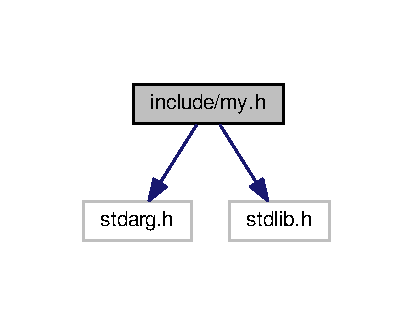
\includegraphics[width=198pt]{my_8h__incl}
\end{center}
\end{figure}
This graph shows which files directly or indirectly include this file\+:
\nopagebreak
\begin{figure}[H]
\begin{center}
\leavevmode
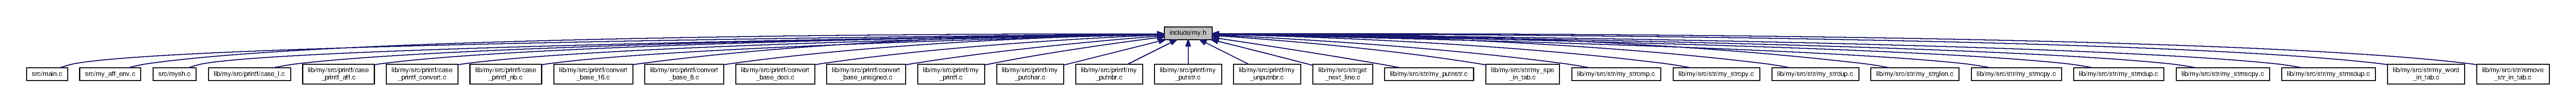
\includegraphics[width=350pt]{my_8h__dep__incl}
\end{center}
\end{figure}
\subsection*{Data Structures}
\begin{DoxyCompactItemize}
\item 
struct \hyperlink{structs__index}{s\+\_\+index}
\item 
struct \hyperlink{structs__struc}{s\+\_\+struc}
\item 
struct \hyperlink{structs__win}{s\+\_\+win}
\item 
struct \hyperlink{structs__getline}{s\+\_\+getline}
\end{DoxyCompactItemize}
\subsection*{Macros}
\begin{DoxyCompactItemize}
\item 
\#define \hyperlink{my_8h_a08b65f6ef2e2a31bf96774acd9a4f923}{S\+I\+Z\+E\+\_\+\+O\+F\+\_\+\+R\+E\+A\+D}~1
\end{DoxyCompactItemize}
\subsection*{Typedefs}
\begin{DoxyCompactItemize}
\item 
typedef struct \hyperlink{structs__index}{s\+\_\+index} \hyperlink{my_8h_a648ad484eb5d7e8f5d781c45b20f874f}{t\+\_\+index}
\item 
typedef struct \hyperlink{structs__struc}{s\+\_\+struc} \hyperlink{my_8h_ac25c8b585b5df2bbafd4bdceafa17eb4}{t\+\_\+struc}
\item 
typedef struct \hyperlink{structs__win}{s\+\_\+win} \hyperlink{my_8h_a09c3907d6f69f2c69f28b45122bd6a4a}{t\+\_\+win}
\item 
typedef struct \hyperlink{structs__getline}{s\+\_\+getline} \hyperlink{my_8h_a1670174b47ab43c748df989ae9ef5984}{t\+\_\+getline}
\end{DoxyCompactItemize}
\subsection*{Functions}
\begin{DoxyCompactItemize}
\item 
int \hyperlink{my_8h_abfc16ef2dad9871456d2f218d60291e5}{my\+\_\+strcmp} (char $\ast$a, char $\ast$b)
\item 
int \hyperlink{my_8h_ac7e9bd08d068851e31a5b6d408004638}{my\+\_\+strlen} (char $\ast$str)
\item 
char $\ast$ \hyperlink{my_8h_ab9c6a1e01382ed13c4e3a38018322282}{my\+\_\+strcpy} (char $\ast$dest, char $\ast$src)
\item 
char $\ast$ \hyperlink{my_8h_a4548135c4f1cfcaeff31c8dabb3692d3}{my\+\_\+strdup} (char $\ast$src)
\item 
char $\ast$ \hyperlink{my_8h_a2ffadb0b379fb240cf69a6e336ee5877}{get\+\_\+next\+\_\+line} (const int fd)
\item 
char $\ast$$\ast$ \hyperlink{my_8h_a80c1db0a8b97ae605ef990e4ab025abd}{my\+\_\+spe\+\_\+in\+\_\+tab} (char $\ast$str, char sep)
\item 
int \hyperlink{my_8h_a4f5b9ec850d1c83fd70299ebc2589700}{my\+\_\+strncmp} (char $\ast$a, char $\ast$b, int nb)
\item 
void \hyperlink{my_8h_a1290d1e8d903e883482237b8446243dc}{my\+\_\+putnstr} (char $\ast$str, int nb)
\item 
char $\ast$ \hyperlink{my_8h_aa470a7e58967778144f7d737bf64c3e8}{my\+\_\+strndup} (char $\ast$src, int nb)
\item 
char $\ast$ \hyperlink{my_8h_a975053956fdec1e94d9c3764d4e15367}{my\+\_\+strncpy} (char $\ast$dest, char $\ast$src, int nb)
\item 
char $\ast$ \hyperlink{my_8h_a04349ba349d2ec7aece9350d01b1eaf1}{my\+\_\+strnsdup} (char $\ast$src, int nb)
\item 
char $\ast$ \hyperlink{my_8h_a649bba7162650b9189f3051c74545b3a}{my\+\_\+strnscpy} (char $\ast$dest, char $\ast$src, int nb)
\item 
void \hyperlink{my_8h_ae07e4d968ee702cb282f6d1235fdecff}{remove\+\_\+str\+\_\+in\+\_\+tab} (char $\ast$$\ast$tab, int x)
\item 
int \hyperlink{my_8h_a1d2d0c1f7e29f013e2bfb4ecece00811}{my\+\_\+tablen} (char $\ast$$\ast$tab)
\item 
int \hyperlink{my_8h_a0fc216c55eb7277a61f446154aa01017}{my\+\_\+strglen} (long $\ast$a)
\item 
int \hyperlink{my_8h_a8ed3cc79947555e7d13c91bbba84c558}{my\+\_\+printf} (const char $\ast$format,...)
\item 
void \hyperlink{my_8h_ac4de74d04dc6e263345755eb62676802}{my\+\_\+putchar} (char c)
\item 
int \hyperlink{my_8h_ac7b78302eb76af4307b2d02f98bd75cb}{my\+\_\+putstr} (char $\ast$str)
\item 
int \hyperlink{my_8h_abe11475be3e899d09dd96ff87e27ea33}{my\+\_\+putnbr} (int nb)
\item 
int \hyperlink{my_8h_a0e2a140625b831447e32a892878b72d7}{my\+\_\+unputnbr} (unsigned int nb)
\item 
int \hyperlink{my_8h_aa6df05dfcbd54dc062af6e56215f656f}{my\+\_\+rev\+\_\+int\+\_\+tab\+\_\+long} (char $\ast$tab, long i)
\item 
void \hyperlink{my_8h_ab228b9450ae618a46ca62d2b1809574f}{my\+\_\+rev\+\_\+int\+\_\+tab\+\_\+un} (char $\ast$tab, long i)
\item 
void \hyperlink{my_8h_a19c537e65b212d78f6088c53687fa546}{my\+\_\+rev\+\_\+int\+\_\+tab} (int $\ast$tab, int i)
\item 
void \hyperlink{my_8h_a1d732a4c44f1469c1fb09eab715773ec}{my\+\_\+rev\+\_\+unint\+\_\+tab} (unsigned int $\ast$tab, int i)
\item 
void \hyperlink{my_8h_afc785712bfc7354145b34cfbc3a33631}{my\+\_\+rev\+\_\+caract\+\_\+nimpr} (int $\ast$tab, int i)
\item 
int \hyperlink{my_8h_ae2b287f062dad36586145d292b4dbf43}{my\+\_\+nb\+\_\+stack} (char n)
\item 
int \hyperlink{my_8h_a44553866ba5bbfc0334e46e5fb65824e}{convert\+\_\+base\+\_\+deci\+\_\+2} (int nb)
\item 
int \hyperlink{my_8h_a60ce8511bf4c820f8b97e85f7217c732}{convert\+\_\+base\+\_\+deci\+\_\+octal} (char strnb, char $\ast$str)
\item 
int \hyperlink{my_8h_adea09e51c1d16f60e2b8b0e82dabc36a}{convert\+\_\+base\+\_\+deci\+\_\+8\+\_\+unint} (unsigned int nb)
\item 
int \hyperlink{my_8h_a8ef7b5028c3c516852da8e8d3bd8f3ab}{convert\+\_\+base\+\_\+deci\+\_\+16\+\_\+un} (unsigned int nb, char $\ast$str)
\item 
int \hyperlink{my_8h_ae76792ea9d72b89dd22b63818937cf6f}{convert\+\_\+base\+\_\+deci\+\_\+16} (long nb, char $\ast$str)
\item 
int \hyperlink{my_8h_a210d12a636371bbb0f25115451e88ea6}{s\+\_\+putstr} (void $\ast$argv, \hyperlink{my_8h_a648ad484eb5d7e8f5d781c45b20f874f}{t\+\_\+index} $\ast$s, const char $\ast$format, const \hyperlink{my_8h_ac25c8b585b5df2bbafd4bdceafa17eb4}{t\+\_\+struc} $\ast$tab)
\item 
int \hyperlink{my_8h_a2ca0365009481f7563e0f8c08cf0e0c9}{case\+\_\+p} (void $\ast$argv, \hyperlink{my_8h_a648ad484eb5d7e8f5d781c45b20f874f}{t\+\_\+index} $\ast$s, const char $\ast$format, const \hyperlink{my_8h_ac25c8b585b5df2bbafd4bdceafa17eb4}{t\+\_\+struc} $\ast$tab)
\item 
int \hyperlink{my_8h_a500cb9fd540fc8337d1bdebb9df56439}{case\+\_\+x} (void $\ast$argv, \hyperlink{my_8h_a648ad484eb5d7e8f5d781c45b20f874f}{t\+\_\+index} $\ast$s, const char $\ast$format, const \hyperlink{my_8h_ac25c8b585b5df2bbafd4bdceafa17eb4}{t\+\_\+struc} $\ast$tab)
\item 
int \hyperlink{my_8h_a3535db665dd6c72c791567112877de4a}{case\+\_\+c} (void $\ast$argv, \hyperlink{my_8h_a648ad484eb5d7e8f5d781c45b20f874f}{t\+\_\+index} $\ast$s, const char $\ast$format, const \hyperlink{my_8h_ac25c8b585b5df2bbafd4bdceafa17eb4}{t\+\_\+struc} $\ast$tab)
\item 
int \hyperlink{my_8h_a91c72293ad0ca640b91b6178fed1ebb2}{case\+\_\+s} (void $\ast$argv, \hyperlink{my_8h_a648ad484eb5d7e8f5d781c45b20f874f}{t\+\_\+index} $\ast$s, const char $\ast$format, const \hyperlink{my_8h_ac25c8b585b5df2bbafd4bdceafa17eb4}{t\+\_\+struc} $\ast$tab)
\item 
int \hyperlink{my_8h_a68fff7b819caa6ed822d928e544b294c}{case\+\_\+b} (void $\ast$argv, \hyperlink{my_8h_a648ad484eb5d7e8f5d781c45b20f874f}{t\+\_\+index} $\ast$s, const char $\ast$format, const \hyperlink{my_8h_ac25c8b585b5df2bbafd4bdceafa17eb4}{t\+\_\+struc} $\ast$tab)
\item 
int \hyperlink{my_8h_af87d61ca079d23141a1d403abdb3bd2d}{case\+\_\+di} (void $\ast$argv, \hyperlink{my_8h_a648ad484eb5d7e8f5d781c45b20f874f}{t\+\_\+index} $\ast$s, const char $\ast$format, const \hyperlink{my_8h_ac25c8b585b5df2bbafd4bdceafa17eb4}{t\+\_\+struc} $\ast$tab)
\item 
int \hyperlink{my_8h_a752193ef66373cc419bfabdcc7850b49}{case\+\_\+o} (void $\ast$argv, \hyperlink{my_8h_a648ad484eb5d7e8f5d781c45b20f874f}{t\+\_\+index} $\ast$s, const char $\ast$format, const \hyperlink{my_8h_ac25c8b585b5df2bbafd4bdceafa17eb4}{t\+\_\+struc} $\ast$tab)
\item 
int \hyperlink{my_8h_a4333d447daeb94aa2c59468dd2dee929}{x\+\_\+case} (void $\ast$argv, \hyperlink{my_8h_a648ad484eb5d7e8f5d781c45b20f874f}{t\+\_\+index} $\ast$s, const char $\ast$format, const \hyperlink{my_8h_ac25c8b585b5df2bbafd4bdceafa17eb4}{t\+\_\+struc} $\ast$tab)
\item 
int \hyperlink{my_8h_ae7a0d4d53622aae2844818b9b55c6a48}{case\+\_\+u} (void $\ast$argv, \hyperlink{my_8h_a648ad484eb5d7e8f5d781c45b20f874f}{t\+\_\+index} $\ast$s, const char $\ast$format, const \hyperlink{my_8h_ac25c8b585b5df2bbafd4bdceafa17eb4}{t\+\_\+struc} $\ast$tab)
\item 
int \hyperlink{my_8h_a83a21528a9e6f2461dba942d6892c1a8}{case\+\_\+pres} (void $\ast$argv, \hyperlink{my_8h_a648ad484eb5d7e8f5d781c45b20f874f}{t\+\_\+index} $\ast$s, const char $\ast$format, const \hyperlink{my_8h_ac25c8b585b5df2bbafd4bdceafa17eb4}{t\+\_\+struc} $\ast$tab)
\item 
int \hyperlink{my_8h_abaafbf096a795ff378896ed44c85bf0e}{case\+\_\+sharp} (void $\ast$argv, \hyperlink{my_8h_a648ad484eb5d7e8f5d781c45b20f874f}{t\+\_\+index} $\ast$s, const char $\ast$format, const \hyperlink{my_8h_ac25c8b585b5df2bbafd4bdceafa17eb4}{t\+\_\+struc} $\ast$tab)
\item 
int \hyperlink{my_8h_ab13cbc229e8177d316dd3d9d88cdb567}{case\+\_\+sharp2} (\hyperlink{my_8h_a648ad484eb5d7e8f5d781c45b20f874f}{t\+\_\+index} $\ast$s, const char $\ast$format, int i, const \hyperlink{my_8h_ac25c8b585b5df2bbafd4bdceafa17eb4}{t\+\_\+struc} $\ast$tab)
\item 
int \hyperlink{my_8h_a013d463656e55e0618a6e1f4d937168a}{case\+\_\+zero} (void $\ast$argv, \hyperlink{my_8h_a648ad484eb5d7e8f5d781c45b20f874f}{t\+\_\+index} $\ast$s, const char $\ast$format, const \hyperlink{my_8h_ac25c8b585b5df2bbafd4bdceafa17eb4}{t\+\_\+struc} $\ast$tab)
\item 
int \hyperlink{my_8h_a4a032b76fd1462824c8617c00826036e}{my\+\_\+putnbrnoaffich} (int nb)
\item 
int \hyperlink{my_8h_a79d3de06392038b9372c01e0114614a0}{my\+\_\+putnbrs} (int nb, int p, int nbr)
\item 
int \hyperlink{my_8h_ab0e9c74dd440e1a52cb7f52fdb13c09c}{my\+\_\+unputnbrnoaffich} (unsigned int nb)
\item 
int \hyperlink{my_8h_a9bbf186c3c7f01218fad6ee69cef6b2d}{my\+\_\+unputnbrs} (unsigned int nb, int p, int nbr)
\item 
int \hyperlink{my_8h_a4861f05079aaf8e8313344b16751a0a6}{case\+\_\+l} (void $\ast$argv, \hyperlink{my_8h_a648ad484eb5d7e8f5d781c45b20f874f}{t\+\_\+index} $\ast$s, const char $\ast$format, const \hyperlink{my_8h_ac25c8b585b5df2bbafd4bdceafa17eb4}{t\+\_\+struc} $\ast$tab)
\item 
int \hyperlink{my_8h_a536c564648bff72a124a93f152da14c3}{my\+\_\+lunputnbr} (long unsigned int nb)
\item 
int \hyperlink{my_8h_a4ea08d997ed58989dca897fefff685dd}{my\+\_\+lputnbr} (long int nb)
\item 
int \hyperlink{my_8h_aceed4b7866a7db390bbc5f95524ebbef}{convert\+\_\+base\+\_\+deci\+\_\+16\+\_\+lun} (long unsigned int nb, char $\ast$str)
\item 
void \hyperlink{my_8h_aaba0b1edc5014a1d679a115792fc3056}{my\+\_\+rev\+\_\+lunint\+\_\+tab} (long unsigned int $\ast$tab, int i)
\item 
int \hyperlink{my_8h_ab1108b223543db15017e7cec0e108b12}{convert\+\_\+base\+\_\+deci\+\_\+8\+\_\+lunint} (long unsigned int nb)
\item 
char $\ast$$\ast$ \hyperlink{my_8h_a7c85d790d5958ef6b7e880acd800fc4f}{my\+\_\+word\+\_\+in\+\_\+tab} (char $\ast$str)
\item 
char $\ast$ \hyperlink{my_8h_add69ea0bdb5fbac8c2bc24631c17cb26}{getbuffer} (char $\ast$buffer, char $\ast$retbuffer)
\item 
char $\ast$ \hyperlink{my_8h_a63c4dde944ff2968597443eaf08c9bc6}{stat\+\_\+in\+\_\+buff} (char $\ast$strtbuffer, char $\ast$buffer, \hyperlink{my_8h_a1670174b47ab43c748df989ae9ef5984}{t\+\_\+getline} $\ast$s, char $\ast$dest)
\item 
void \hyperlink{my_8h_a9bf3a9107dbcf7a29220551c1fdd07ce}{where\+\_\+my\+\_\+buff\+\_\+end} (char $\ast$statbuffer, char $\ast$stockstat, int j)
\item 
void \hyperlink{my_8h_a922043af008f3521c98c490bfb92b0b7}{my\+\_\+gstrcpy} (char $\ast$buffer, char $\ast$stockstat, \hyperlink{my_8h_a1670174b47ab43c748df989ae9ef5984}{t\+\_\+getline} $\ast$s, char $\ast$dest)
\end{DoxyCompactItemize}


\subsection{Macro Definition Documentation}
\hypertarget{my_8h_a08b65f6ef2e2a31bf96774acd9a4f923}{\index{my.\+h@{my.\+h}!S\+I\+Z\+E\+\_\+\+O\+F\+\_\+\+R\+E\+A\+D@{S\+I\+Z\+E\+\_\+\+O\+F\+\_\+\+R\+E\+A\+D}}
\index{S\+I\+Z\+E\+\_\+\+O\+F\+\_\+\+R\+E\+A\+D@{S\+I\+Z\+E\+\_\+\+O\+F\+\_\+\+R\+E\+A\+D}!my.\+h@{my.\+h}}
\subsubsection[{S\+I\+Z\+E\+\_\+\+O\+F\+\_\+\+R\+E\+A\+D}]{\setlength{\rightskip}{0pt plus 5cm}\#define S\+I\+Z\+E\+\_\+\+O\+F\+\_\+\+R\+E\+A\+D~1}}\label{my_8h_a08b65f6ef2e2a31bf96774acd9a4f923}


Definition at line 155 of file my.\+h.



\subsection{Typedef Documentation}
\hypertarget{my_8h_a1670174b47ab43c748df989ae9ef5984}{\index{my.\+h@{my.\+h}!t\+\_\+getline@{t\+\_\+getline}}
\index{t\+\_\+getline@{t\+\_\+getline}!my.\+h@{my.\+h}}
\subsubsection[{t\+\_\+getline}]{\setlength{\rightskip}{0pt plus 5cm}typedef struct {\bf s\+\_\+getline}		 {\bf t\+\_\+getline}}}\label{my_8h_a1670174b47ab43c748df989ae9ef5984}
\hypertarget{my_8h_a648ad484eb5d7e8f5d781c45b20f874f}{\index{my.\+h@{my.\+h}!t\+\_\+index@{t\+\_\+index}}
\index{t\+\_\+index@{t\+\_\+index}!my.\+h@{my.\+h}}
\subsubsection[{t\+\_\+index}]{\setlength{\rightskip}{0pt plus 5cm}typedef struct {\bf s\+\_\+index}			 {\bf t\+\_\+index}}}\label{my_8h_a648ad484eb5d7e8f5d781c45b20f874f}
\hypertarget{my_8h_ac25c8b585b5df2bbafd4bdceafa17eb4}{\index{my.\+h@{my.\+h}!t\+\_\+struc@{t\+\_\+struc}}
\index{t\+\_\+struc@{t\+\_\+struc}!my.\+h@{my.\+h}}
\subsubsection[{t\+\_\+struc}]{\setlength{\rightskip}{0pt plus 5cm}typedef struct {\bf s\+\_\+struc}			 {\bf t\+\_\+struc}}}\label{my_8h_ac25c8b585b5df2bbafd4bdceafa17eb4}
\hypertarget{my_8h_a09c3907d6f69f2c69f28b45122bd6a4a}{\index{my.\+h@{my.\+h}!t\+\_\+win@{t\+\_\+win}}
\index{t\+\_\+win@{t\+\_\+win}!my.\+h@{my.\+h}}
\subsubsection[{t\+\_\+win}]{\setlength{\rightskip}{0pt plus 5cm}typedef struct {\bf s\+\_\+win}		 {\bf t\+\_\+win}}}\label{my_8h_a09c3907d6f69f2c69f28b45122bd6a4a}


\subsection{Function Documentation}
\hypertarget{my_8h_a68fff7b819caa6ed822d928e544b294c}{\index{my.\+h@{my.\+h}!case\+\_\+b@{case\+\_\+b}}
\index{case\+\_\+b@{case\+\_\+b}!my.\+h@{my.\+h}}
\subsubsection[{case\+\_\+b}]{\setlength{\rightskip}{0pt plus 5cm}int case\+\_\+b (
\begin{DoxyParamCaption}
\item[{void $\ast$}]{argv, }
\item[{{\bf t\+\_\+index} $\ast$}]{s, }
\item[{const char $\ast$}]{format, }
\item[{const {\bf t\+\_\+struc} $\ast$}]{tab}
\end{DoxyParamCaption}
)}}\label{my_8h_a68fff7b819caa6ed822d928e544b294c}


Definition at line 13 of file case\+\_\+printf\+\_\+nb.\+c.

\hypertarget{my_8h_a3535db665dd6c72c791567112877de4a}{\index{my.\+h@{my.\+h}!case\+\_\+c@{case\+\_\+c}}
\index{case\+\_\+c@{case\+\_\+c}!my.\+h@{my.\+h}}
\subsubsection[{case\+\_\+c}]{\setlength{\rightskip}{0pt plus 5cm}int case\+\_\+c (
\begin{DoxyParamCaption}
\item[{void $\ast$}]{argv, }
\item[{{\bf t\+\_\+index} $\ast$}]{s, }
\item[{const char $\ast$}]{format, }
\item[{const {\bf t\+\_\+struc} $\ast$}]{tab}
\end{DoxyParamCaption}
)}}\label{my_8h_a3535db665dd6c72c791567112877de4a}


Definition at line 66 of file case\+\_\+printf\+\_\+aff.\+c.

\hypertarget{my_8h_af87d61ca079d23141a1d403abdb3bd2d}{\index{my.\+h@{my.\+h}!case\+\_\+di@{case\+\_\+di}}
\index{case\+\_\+di@{case\+\_\+di}!my.\+h@{my.\+h}}
\subsubsection[{case\+\_\+di}]{\setlength{\rightskip}{0pt plus 5cm}int case\+\_\+di (
\begin{DoxyParamCaption}
\item[{void $\ast$}]{argv, }
\item[{{\bf t\+\_\+index} $\ast$}]{s, }
\item[{const char $\ast$}]{format, }
\item[{const {\bf t\+\_\+struc} $\ast$}]{tab}
\end{DoxyParamCaption}
)}}\label{my_8h_af87d61ca079d23141a1d403abdb3bd2d}


Definition at line 27 of file case\+\_\+printf\+\_\+nb.\+c.

\hypertarget{my_8h_a4861f05079aaf8e8313344b16751a0a6}{\index{my.\+h@{my.\+h}!case\+\_\+l@{case\+\_\+l}}
\index{case\+\_\+l@{case\+\_\+l}!my.\+h@{my.\+h}}
\subsubsection[{case\+\_\+l}]{\setlength{\rightskip}{0pt plus 5cm}int case\+\_\+l (
\begin{DoxyParamCaption}
\item[{void $\ast$}]{argv, }
\item[{{\bf t\+\_\+index} $\ast$}]{s, }
\item[{const char $\ast$}]{format, }
\item[{const {\bf t\+\_\+struc} $\ast$}]{tab}
\end{DoxyParamCaption}
)}}\label{my_8h_a4861f05079aaf8e8313344b16751a0a6}


Definition at line 13 of file case\+\_\+l.\+c.

\hypertarget{my_8h_a752193ef66373cc419bfabdcc7850b49}{\index{my.\+h@{my.\+h}!case\+\_\+o@{case\+\_\+o}}
\index{case\+\_\+o@{case\+\_\+o}!my.\+h@{my.\+h}}
\subsubsection[{case\+\_\+o}]{\setlength{\rightskip}{0pt plus 5cm}int case\+\_\+o (
\begin{DoxyParamCaption}
\item[{void $\ast$}]{argv, }
\item[{{\bf t\+\_\+index} $\ast$}]{s, }
\item[{const char $\ast$}]{format, }
\item[{const {\bf t\+\_\+struc} $\ast$}]{tab}
\end{DoxyParamCaption}
)}}\label{my_8h_a752193ef66373cc419bfabdcc7850b49}


Definition at line 44 of file case\+\_\+printf\+\_\+nb.\+c.

\hypertarget{my_8h_a2ca0365009481f7563e0f8c08cf0e0c9}{\index{my.\+h@{my.\+h}!case\+\_\+p@{case\+\_\+p}}
\index{case\+\_\+p@{case\+\_\+p}!my.\+h@{my.\+h}}
\subsubsection[{case\+\_\+p}]{\setlength{\rightskip}{0pt plus 5cm}int case\+\_\+p (
\begin{DoxyParamCaption}
\item[{void $\ast$}]{argv, }
\item[{{\bf t\+\_\+index} $\ast$}]{s, }
\item[{const char $\ast$}]{format, }
\item[{const {\bf t\+\_\+struc} $\ast$}]{tab}
\end{DoxyParamCaption}
)}}\label{my_8h_a2ca0365009481f7563e0f8c08cf0e0c9}


Definition at line 35 of file case\+\_\+printf\+\_\+aff.\+c.

\hypertarget{my_8h_a83a21528a9e6f2461dba942d6892c1a8}{\index{my.\+h@{my.\+h}!case\+\_\+pres@{case\+\_\+pres}}
\index{case\+\_\+pres@{case\+\_\+pres}!my.\+h@{my.\+h}}
\subsubsection[{case\+\_\+pres}]{\setlength{\rightskip}{0pt plus 5cm}int case\+\_\+pres (
\begin{DoxyParamCaption}
\item[{void $\ast$}]{argv, }
\item[{{\bf t\+\_\+index} $\ast$}]{s, }
\item[{const char $\ast$}]{format, }
\item[{const {\bf t\+\_\+struc} $\ast$}]{tab}
\end{DoxyParamCaption}
)}}\label{my_8h_a83a21528a9e6f2461dba942d6892c1a8}


Definition at line 13 of file case\+\_\+printf\+\_\+convert.\+c.

\hypertarget{my_8h_a91c72293ad0ca640b91b6178fed1ebb2}{\index{my.\+h@{my.\+h}!case\+\_\+s@{case\+\_\+s}}
\index{case\+\_\+s@{case\+\_\+s}!my.\+h@{my.\+h}}
\subsubsection[{case\+\_\+s}]{\setlength{\rightskip}{0pt plus 5cm}int case\+\_\+s (
\begin{DoxyParamCaption}
\item[{void $\ast$}]{argv, }
\item[{{\bf t\+\_\+index} $\ast$}]{s, }
\item[{const char $\ast$}]{format, }
\item[{const {\bf t\+\_\+struc} $\ast$}]{tab}
\end{DoxyParamCaption}
)}}\label{my_8h_a91c72293ad0ca640b91b6178fed1ebb2}


Definition at line 79 of file case\+\_\+printf\+\_\+aff.\+c.

\hypertarget{my_8h_abaafbf096a795ff378896ed44c85bf0e}{\index{my.\+h@{my.\+h}!case\+\_\+sharp@{case\+\_\+sharp}}
\index{case\+\_\+sharp@{case\+\_\+sharp}!my.\+h@{my.\+h}}
\subsubsection[{case\+\_\+sharp}]{\setlength{\rightskip}{0pt plus 5cm}int case\+\_\+sharp (
\begin{DoxyParamCaption}
\item[{void $\ast$}]{argv, }
\item[{{\bf t\+\_\+index} $\ast$}]{s, }
\item[{const char $\ast$}]{format, }
\item[{const {\bf t\+\_\+struc} $\ast$}]{tab}
\end{DoxyParamCaption}
)}}\label{my_8h_abaafbf096a795ff378896ed44c85bf0e}


Definition at line 42 of file case\+\_\+printf\+\_\+convert.\+c.

\hypertarget{my_8h_ab13cbc229e8177d316dd3d9d88cdb567}{\index{my.\+h@{my.\+h}!case\+\_\+sharp2@{case\+\_\+sharp2}}
\index{case\+\_\+sharp2@{case\+\_\+sharp2}!my.\+h@{my.\+h}}
\subsubsection[{case\+\_\+sharp2}]{\setlength{\rightskip}{0pt plus 5cm}int case\+\_\+sharp2 (
\begin{DoxyParamCaption}
\item[{{\bf t\+\_\+index} $\ast$}]{s, }
\item[{const char $\ast$}]{format, }
\item[{int}]{i, }
\item[{const {\bf t\+\_\+struc} $\ast$}]{tab}
\end{DoxyParamCaption}
)}}\label{my_8h_ab13cbc229e8177d316dd3d9d88cdb567}


Definition at line 24 of file case\+\_\+printf\+\_\+convert.\+c.

\hypertarget{my_8h_ae7a0d4d53622aae2844818b9b55c6a48}{\index{my.\+h@{my.\+h}!case\+\_\+u@{case\+\_\+u}}
\index{case\+\_\+u@{case\+\_\+u}!my.\+h@{my.\+h}}
\subsubsection[{case\+\_\+u}]{\setlength{\rightskip}{0pt plus 5cm}int case\+\_\+u (
\begin{DoxyParamCaption}
\item[{void $\ast$}]{argv, }
\item[{{\bf t\+\_\+index} $\ast$}]{s, }
\item[{const char $\ast$}]{format, }
\item[{const {\bf t\+\_\+struc} $\ast$}]{tab}
\end{DoxyParamCaption}
)}}\label{my_8h_ae7a0d4d53622aae2844818b9b55c6a48}


Definition at line 79 of file case\+\_\+printf\+\_\+nb.\+c.

\hypertarget{my_8h_a500cb9fd540fc8337d1bdebb9df56439}{\index{my.\+h@{my.\+h}!case\+\_\+x@{case\+\_\+x}}
\index{case\+\_\+x@{case\+\_\+x}!my.\+h@{my.\+h}}
\subsubsection[{case\+\_\+x}]{\setlength{\rightskip}{0pt plus 5cm}int case\+\_\+x (
\begin{DoxyParamCaption}
\item[{void $\ast$}]{argv, }
\item[{{\bf t\+\_\+index} $\ast$}]{s, }
\item[{const char $\ast$}]{format, }
\item[{const {\bf t\+\_\+struc} $\ast$}]{tab}
\end{DoxyParamCaption}
)}}\label{my_8h_a500cb9fd540fc8337d1bdebb9df56439}


Definition at line 49 of file case\+\_\+printf\+\_\+aff.\+c.

\hypertarget{my_8h_a013d463656e55e0618a6e1f4d937168a}{\index{my.\+h@{my.\+h}!case\+\_\+zero@{case\+\_\+zero}}
\index{case\+\_\+zero@{case\+\_\+zero}!my.\+h@{my.\+h}}
\subsubsection[{case\+\_\+zero}]{\setlength{\rightskip}{0pt plus 5cm}int case\+\_\+zero (
\begin{DoxyParamCaption}
\item[{void $\ast$}]{argv, }
\item[{{\bf t\+\_\+index} $\ast$}]{s, }
\item[{const char $\ast$}]{format, }
\item[{const {\bf t\+\_\+struc} $\ast$}]{tab}
\end{DoxyParamCaption}
)}}\label{my_8h_a013d463656e55e0618a6e1f4d937168a}


Definition at line 63 of file case\+\_\+printf\+\_\+convert.\+c.

\hypertarget{my_8h_ae76792ea9d72b89dd22b63818937cf6f}{\index{my.\+h@{my.\+h}!convert\+\_\+base\+\_\+deci\+\_\+16@{convert\+\_\+base\+\_\+deci\+\_\+16}}
\index{convert\+\_\+base\+\_\+deci\+\_\+16@{convert\+\_\+base\+\_\+deci\+\_\+16}!my.\+h@{my.\+h}}
\subsubsection[{convert\+\_\+base\+\_\+deci\+\_\+16}]{\setlength{\rightskip}{0pt plus 5cm}int convert\+\_\+base\+\_\+deci\+\_\+16 (
\begin{DoxyParamCaption}
\item[{long}]{nb, }
\item[{char $\ast$}]{str}
\end{DoxyParamCaption}
)}}\label{my_8h_ae76792ea9d72b89dd22b63818937cf6f}


Definition at line 67 of file convert\+\_\+base\+\_\+deci.\+c.

\hypertarget{my_8h_aceed4b7866a7db390bbc5f95524ebbef}{\index{my.\+h@{my.\+h}!convert\+\_\+base\+\_\+deci\+\_\+16\+\_\+lun@{convert\+\_\+base\+\_\+deci\+\_\+16\+\_\+lun}}
\index{convert\+\_\+base\+\_\+deci\+\_\+16\+\_\+lun@{convert\+\_\+base\+\_\+deci\+\_\+16\+\_\+lun}!my.\+h@{my.\+h}}
\subsubsection[{convert\+\_\+base\+\_\+deci\+\_\+16\+\_\+lun}]{\setlength{\rightskip}{0pt plus 5cm}int convert\+\_\+base\+\_\+deci\+\_\+16\+\_\+lun (
\begin{DoxyParamCaption}
\item[{long unsigned int}]{nb, }
\item[{char $\ast$}]{str}
\end{DoxyParamCaption}
)}}\label{my_8h_aceed4b7866a7db390bbc5f95524ebbef}


Definition at line 14 of file convert\+\_\+base\+\_\+unsigned.\+c.

\hypertarget{my_8h_a8ef7b5028c3c516852da8e8d3bd8f3ab}{\index{my.\+h@{my.\+h}!convert\+\_\+base\+\_\+deci\+\_\+16\+\_\+un@{convert\+\_\+base\+\_\+deci\+\_\+16\+\_\+un}}
\index{convert\+\_\+base\+\_\+deci\+\_\+16\+\_\+un@{convert\+\_\+base\+\_\+deci\+\_\+16\+\_\+un}!my.\+h@{my.\+h}}
\subsubsection[{convert\+\_\+base\+\_\+deci\+\_\+16\+\_\+un}]{\setlength{\rightskip}{0pt plus 5cm}int convert\+\_\+base\+\_\+deci\+\_\+16\+\_\+un (
\begin{DoxyParamCaption}
\item[{unsigned int}]{nb, }
\item[{char $\ast$}]{str}
\end{DoxyParamCaption}
)}}\label{my_8h_a8ef7b5028c3c516852da8e8d3bd8f3ab}


Definition at line 40 of file convert\+\_\+base\+\_\+deci.\+c.

\hypertarget{my_8h_a44553866ba5bbfc0334e46e5fb65824e}{\index{my.\+h@{my.\+h}!convert\+\_\+base\+\_\+deci\+\_\+2@{convert\+\_\+base\+\_\+deci\+\_\+2}}
\index{convert\+\_\+base\+\_\+deci\+\_\+2@{convert\+\_\+base\+\_\+deci\+\_\+2}!my.\+h@{my.\+h}}
\subsubsection[{convert\+\_\+base\+\_\+deci\+\_\+2}]{\setlength{\rightskip}{0pt plus 5cm}int convert\+\_\+base\+\_\+deci\+\_\+2 (
\begin{DoxyParamCaption}
\item[{int}]{nb}
\end{DoxyParamCaption}
)}}\label{my_8h_a44553866ba5bbfc0334e46e5fb65824e}


Definition at line 48 of file convert\+\_\+base\+\_\+8.\+c.

\hypertarget{my_8h_ab1108b223543db15017e7cec0e108b12}{\index{my.\+h@{my.\+h}!convert\+\_\+base\+\_\+deci\+\_\+8\+\_\+lunint@{convert\+\_\+base\+\_\+deci\+\_\+8\+\_\+lunint}}
\index{convert\+\_\+base\+\_\+deci\+\_\+8\+\_\+lunint@{convert\+\_\+base\+\_\+deci\+\_\+8\+\_\+lunint}!my.\+h@{my.\+h}}
\subsubsection[{convert\+\_\+base\+\_\+deci\+\_\+8\+\_\+lunint}]{\setlength{\rightskip}{0pt plus 5cm}int convert\+\_\+base\+\_\+deci\+\_\+8\+\_\+lunint (
\begin{DoxyParamCaption}
\item[{long unsigned int}]{nb}
\end{DoxyParamCaption}
)}}\label{my_8h_ab1108b223543db15017e7cec0e108b12}


Definition at line 51 of file convert\+\_\+base\+\_\+unsigned.\+c.

\hypertarget{my_8h_adea09e51c1d16f60e2b8b0e82dabc36a}{\index{my.\+h@{my.\+h}!convert\+\_\+base\+\_\+deci\+\_\+8\+\_\+unint@{convert\+\_\+base\+\_\+deci\+\_\+8\+\_\+unint}}
\index{convert\+\_\+base\+\_\+deci\+\_\+8\+\_\+unint@{convert\+\_\+base\+\_\+deci\+\_\+8\+\_\+unint}!my.\+h@{my.\+h}}
\subsubsection[{convert\+\_\+base\+\_\+deci\+\_\+8\+\_\+unint}]{\setlength{\rightskip}{0pt plus 5cm}int convert\+\_\+base\+\_\+deci\+\_\+8\+\_\+unint (
\begin{DoxyParamCaption}
\item[{unsigned int}]{nb}
\end{DoxyParamCaption}
)}}\label{my_8h_adea09e51c1d16f60e2b8b0e82dabc36a}


Definition at line 14 of file convert\+\_\+base\+\_\+deci.\+c.

\hypertarget{my_8h_a60ce8511bf4c820f8b97e85f7217c732}{\index{my.\+h@{my.\+h}!convert\+\_\+base\+\_\+deci\+\_\+octal@{convert\+\_\+base\+\_\+deci\+\_\+octal}}
\index{convert\+\_\+base\+\_\+deci\+\_\+octal@{convert\+\_\+base\+\_\+deci\+\_\+octal}!my.\+h@{my.\+h}}
\subsubsection[{convert\+\_\+base\+\_\+deci\+\_\+octal}]{\setlength{\rightskip}{0pt plus 5cm}int convert\+\_\+base\+\_\+deci\+\_\+octal (
\begin{DoxyParamCaption}
\item[{char}]{strnb, }
\item[{char $\ast$}]{str}
\end{DoxyParamCaption}
)}}\label{my_8h_a60ce8511bf4c820f8b97e85f7217c732}


Definition at line 75 of file convert\+\_\+base\+\_\+8.\+c.

\hypertarget{my_8h_a2ffadb0b379fb240cf69a6e336ee5877}{\index{my.\+h@{my.\+h}!get\+\_\+next\+\_\+line@{get\+\_\+next\+\_\+line}}
\index{get\+\_\+next\+\_\+line@{get\+\_\+next\+\_\+line}!my.\+h@{my.\+h}}
\subsubsection[{get\+\_\+next\+\_\+line}]{\setlength{\rightskip}{0pt plus 5cm}char $\ast$ get\+\_\+next\+\_\+line (
\begin{DoxyParamCaption}
\item[{const int}]{fd}
\end{DoxyParamCaption}
)}}\label{my_8h_a2ffadb0b379fb240cf69a6e336ee5877}


Definition at line 81 of file get\+\_\+next\+\_\+line.\+c.

\hypertarget{my_8h_add69ea0bdb5fbac8c2bc24631c17cb26}{\index{my.\+h@{my.\+h}!getbuffer@{getbuffer}}
\index{getbuffer@{getbuffer}!my.\+h@{my.\+h}}
\subsubsection[{getbuffer}]{\setlength{\rightskip}{0pt plus 5cm}char$\ast$ getbuffer (
\begin{DoxyParamCaption}
\item[{char $\ast$}]{buffer, }
\item[{char $\ast$}]{retbuffer}
\end{DoxyParamCaption}
)}}\label{my_8h_add69ea0bdb5fbac8c2bc24631c17cb26}
\hypertarget{my_8h_a922043af008f3521c98c490bfb92b0b7}{\index{my.\+h@{my.\+h}!my\+\_\+gstrcpy@{my\+\_\+gstrcpy}}
\index{my\+\_\+gstrcpy@{my\+\_\+gstrcpy}!my.\+h@{my.\+h}}
\subsubsection[{my\+\_\+gstrcpy}]{\setlength{\rightskip}{0pt plus 5cm}void my\+\_\+gstrcpy (
\begin{DoxyParamCaption}
\item[{char $\ast$}]{buffer, }
\item[{char $\ast$}]{stockstat, }
\item[{{\bf t\+\_\+getline} $\ast$}]{s, }
\item[{char $\ast$}]{dest}
\end{DoxyParamCaption}
)}}\label{my_8h_a922043af008f3521c98c490bfb92b0b7}


Definition at line 29 of file get\+\_\+next\+\_\+line.\+c.

\hypertarget{my_8h_a4ea08d997ed58989dca897fefff685dd}{\index{my.\+h@{my.\+h}!my\+\_\+lputnbr@{my\+\_\+lputnbr}}
\index{my\+\_\+lputnbr@{my\+\_\+lputnbr}!my.\+h@{my.\+h}}
\subsubsection[{my\+\_\+lputnbr}]{\setlength{\rightskip}{0pt plus 5cm}int my\+\_\+lputnbr (
\begin{DoxyParamCaption}
\item[{long int}]{nb}
\end{DoxyParamCaption}
)}}\label{my_8h_a4ea08d997ed58989dca897fefff685dd}


Definition at line 77 of file my\+\_\+unputnbr.\+c.

\hypertarget{my_8h_a536c564648bff72a124a93f152da14c3}{\index{my.\+h@{my.\+h}!my\+\_\+lunputnbr@{my\+\_\+lunputnbr}}
\index{my\+\_\+lunputnbr@{my\+\_\+lunputnbr}!my.\+h@{my.\+h}}
\subsubsection[{my\+\_\+lunputnbr}]{\setlength{\rightskip}{0pt plus 5cm}int my\+\_\+lunputnbr (
\begin{DoxyParamCaption}
\item[{long unsigned int}]{nb}
\end{DoxyParamCaption}
)}}\label{my_8h_a536c564648bff72a124a93f152da14c3}


Definition at line 91 of file my\+\_\+putnbr.\+c.

\hypertarget{my_8h_ae2b287f062dad36586145d292b4dbf43}{\index{my.\+h@{my.\+h}!my\+\_\+nb\+\_\+stack@{my\+\_\+nb\+\_\+stack}}
\index{my\+\_\+nb\+\_\+stack@{my\+\_\+nb\+\_\+stack}!my.\+h@{my.\+h}}
\subsubsection[{my\+\_\+nb\+\_\+stack}]{\setlength{\rightskip}{0pt plus 5cm}int my\+\_\+nb\+\_\+stack (
\begin{DoxyParamCaption}
\item[{char}]{n}
\end{DoxyParamCaption}
)}}\label{my_8h_ae2b287f062dad36586145d292b4dbf43}


Definition at line 39 of file convert\+\_\+base\+\_\+8.\+c.

\hypertarget{my_8h_a8ed3cc79947555e7d13c91bbba84c558}{\index{my.\+h@{my.\+h}!my\+\_\+printf@{my\+\_\+printf}}
\index{my\+\_\+printf@{my\+\_\+printf}!my.\+h@{my.\+h}}
\subsubsection[{my\+\_\+printf}]{\setlength{\rightskip}{0pt plus 5cm}int my\+\_\+printf (
\begin{DoxyParamCaption}
\item[{const char $\ast$}]{format, }
\item[{}]{...}
\end{DoxyParamCaption}
)}}\label{my_8h_a8ed3cc79947555e7d13c91bbba84c558}


Definition at line 57 of file my\+\_\+printf.\+c.

\hypertarget{my_8h_ac4de74d04dc6e263345755eb62676802}{\index{my.\+h@{my.\+h}!my\+\_\+putchar@{my\+\_\+putchar}}
\index{my\+\_\+putchar@{my\+\_\+putchar}!my.\+h@{my.\+h}}
\subsubsection[{my\+\_\+putchar}]{\setlength{\rightskip}{0pt plus 5cm}void my\+\_\+putchar (
\begin{DoxyParamCaption}
\item[{char}]{c}
\end{DoxyParamCaption}
)}}\label{my_8h_ac4de74d04dc6e263345755eb62676802}


Definition at line 15 of file my\+\_\+putchar.\+c.

\hypertarget{my_8h_abe11475be3e899d09dd96ff87e27ea33}{\index{my.\+h@{my.\+h}!my\+\_\+putnbr@{my\+\_\+putnbr}}
\index{my\+\_\+putnbr@{my\+\_\+putnbr}!my.\+h@{my.\+h}}
\subsubsection[{my\+\_\+putnbr}]{\setlength{\rightskip}{0pt plus 5cm}int my\+\_\+putnbr (
\begin{DoxyParamCaption}
\item[{int}]{nb}
\end{DoxyParamCaption}
)}}\label{my_8h_abe11475be3e899d09dd96ff87e27ea33}


Definition at line 13 of file my\+\_\+putnbr.\+c.

\hypertarget{my_8h_a4a032b76fd1462824c8617c00826036e}{\index{my.\+h@{my.\+h}!my\+\_\+putnbrnoaffich@{my\+\_\+putnbrnoaffich}}
\index{my\+\_\+putnbrnoaffich@{my\+\_\+putnbrnoaffich}!my.\+h@{my.\+h}}
\subsubsection[{my\+\_\+putnbrnoaffich}]{\setlength{\rightskip}{0pt plus 5cm}int my\+\_\+putnbrnoaffich (
\begin{DoxyParamCaption}
\item[{int}]{nb}
\end{DoxyParamCaption}
)}}\label{my_8h_a4a032b76fd1462824c8617c00826036e}


Definition at line 41 of file my\+\_\+putnbr.\+c.

\hypertarget{my_8h_a79d3de06392038b9372c01e0114614a0}{\index{my.\+h@{my.\+h}!my\+\_\+putnbrs@{my\+\_\+putnbrs}}
\index{my\+\_\+putnbrs@{my\+\_\+putnbrs}!my.\+h@{my.\+h}}
\subsubsection[{my\+\_\+putnbrs}]{\setlength{\rightskip}{0pt plus 5cm}int my\+\_\+putnbrs (
\begin{DoxyParamCaption}
\item[{int}]{nb, }
\item[{int}]{p, }
\item[{int}]{nbr}
\end{DoxyParamCaption}
)}}\label{my_8h_a79d3de06392038b9372c01e0114614a0}


Definition at line 65 of file my\+\_\+putnbr.\+c.

\hypertarget{my_8h_a1290d1e8d903e883482237b8446243dc}{\index{my.\+h@{my.\+h}!my\+\_\+putnstr@{my\+\_\+putnstr}}
\index{my\+\_\+putnstr@{my\+\_\+putnstr}!my.\+h@{my.\+h}}
\subsubsection[{my\+\_\+putnstr}]{\setlength{\rightskip}{0pt plus 5cm}void my\+\_\+putnstr (
\begin{DoxyParamCaption}
\item[{char $\ast$}]{str, }
\item[{int}]{nb}
\end{DoxyParamCaption}
)}}\label{my_8h_a1290d1e8d903e883482237b8446243dc}


Definition at line 13 of file my\+\_\+putnstr.\+c.

\hypertarget{my_8h_ac7b78302eb76af4307b2d02f98bd75cb}{\index{my.\+h@{my.\+h}!my\+\_\+putstr@{my\+\_\+putstr}}
\index{my\+\_\+putstr@{my\+\_\+putstr}!my.\+h@{my.\+h}}
\subsubsection[{my\+\_\+putstr}]{\setlength{\rightskip}{0pt plus 5cm}int my\+\_\+putstr (
\begin{DoxyParamCaption}
\item[{char $\ast$}]{str}
\end{DoxyParamCaption}
)}}\label{my_8h_ac7b78302eb76af4307b2d02f98bd75cb}


Definition at line 13 of file my\+\_\+putstr.\+c.

\hypertarget{my_8h_afc785712bfc7354145b34cfbc3a33631}{\index{my.\+h@{my.\+h}!my\+\_\+rev\+\_\+caract\+\_\+nimpr@{my\+\_\+rev\+\_\+caract\+\_\+nimpr}}
\index{my\+\_\+rev\+\_\+caract\+\_\+nimpr@{my\+\_\+rev\+\_\+caract\+\_\+nimpr}!my.\+h@{my.\+h}}
\subsubsection[{my\+\_\+rev\+\_\+caract\+\_\+nimpr}]{\setlength{\rightskip}{0pt plus 5cm}void my\+\_\+rev\+\_\+caract\+\_\+nimpr (
\begin{DoxyParamCaption}
\item[{int $\ast$}]{tab, }
\item[{int}]{i}
\end{DoxyParamCaption}
)}}\label{my_8h_afc785712bfc7354145b34cfbc3a33631}


Definition at line 24 of file convert\+\_\+base\+\_\+8.\+c.

\hypertarget{my_8h_a19c537e65b212d78f6088c53687fa546}{\index{my.\+h@{my.\+h}!my\+\_\+rev\+\_\+int\+\_\+tab@{my\+\_\+rev\+\_\+int\+\_\+tab}}
\index{my\+\_\+rev\+\_\+int\+\_\+tab@{my\+\_\+rev\+\_\+int\+\_\+tab}!my.\+h@{my.\+h}}
\subsubsection[{my\+\_\+rev\+\_\+int\+\_\+tab}]{\setlength{\rightskip}{0pt plus 5cm}void my\+\_\+rev\+\_\+int\+\_\+tab (
\begin{DoxyParamCaption}
\item[{int $\ast$}]{tab, }
\item[{int}]{i}
\end{DoxyParamCaption}
)}}\label{my_8h_a19c537e65b212d78f6088c53687fa546}


Definition at line 54 of file convert\+\_\+base\+\_\+16.\+c.

\hypertarget{my_8h_aa6df05dfcbd54dc062af6e56215f656f}{\index{my.\+h@{my.\+h}!my\+\_\+rev\+\_\+int\+\_\+tab\+\_\+long@{my\+\_\+rev\+\_\+int\+\_\+tab\+\_\+long}}
\index{my\+\_\+rev\+\_\+int\+\_\+tab\+\_\+long@{my\+\_\+rev\+\_\+int\+\_\+tab\+\_\+long}!my.\+h@{my.\+h}}
\subsubsection[{my\+\_\+rev\+\_\+int\+\_\+tab\+\_\+long}]{\setlength{\rightskip}{0pt plus 5cm}int my\+\_\+rev\+\_\+int\+\_\+tab\+\_\+long (
\begin{DoxyParamCaption}
\item[{char $\ast$}]{tab, }
\item[{long}]{i}
\end{DoxyParamCaption}
)}}\label{my_8h_aa6df05dfcbd54dc062af6e56215f656f}


Definition at line 23 of file convert\+\_\+base\+\_\+16.\+c.

\hypertarget{my_8h_ab228b9450ae618a46ca62d2b1809574f}{\index{my.\+h@{my.\+h}!my\+\_\+rev\+\_\+int\+\_\+tab\+\_\+un@{my\+\_\+rev\+\_\+int\+\_\+tab\+\_\+un}}
\index{my\+\_\+rev\+\_\+int\+\_\+tab\+\_\+un@{my\+\_\+rev\+\_\+int\+\_\+tab\+\_\+un}!my.\+h@{my.\+h}}
\subsubsection[{my\+\_\+rev\+\_\+int\+\_\+tab\+\_\+un}]{\setlength{\rightskip}{0pt plus 5cm}void my\+\_\+rev\+\_\+int\+\_\+tab\+\_\+un (
\begin{DoxyParamCaption}
\item[{char $\ast$}]{tab, }
\item[{long}]{i}
\end{DoxyParamCaption}
)}}\label{my_8h_ab228b9450ae618a46ca62d2b1809574f}


Definition at line 44 of file convert\+\_\+base\+\_\+16.\+c.

\hypertarget{my_8h_aaba0b1edc5014a1d679a115792fc3056}{\index{my.\+h@{my.\+h}!my\+\_\+rev\+\_\+lunint\+\_\+tab@{my\+\_\+rev\+\_\+lunint\+\_\+tab}}
\index{my\+\_\+rev\+\_\+lunint\+\_\+tab@{my\+\_\+rev\+\_\+lunint\+\_\+tab}!my.\+h@{my.\+h}}
\subsubsection[{my\+\_\+rev\+\_\+lunint\+\_\+tab}]{\setlength{\rightskip}{0pt plus 5cm}void my\+\_\+rev\+\_\+lunint\+\_\+tab (
\begin{DoxyParamCaption}
\item[{long unsigned int $\ast$}]{tab, }
\item[{int}]{i}
\end{DoxyParamCaption}
)}}\label{my_8h_aaba0b1edc5014a1d679a115792fc3056}


Definition at line 41 of file convert\+\_\+base\+\_\+unsigned.\+c.

\hypertarget{my_8h_a1d732a4c44f1469c1fb09eab715773ec}{\index{my.\+h@{my.\+h}!my\+\_\+rev\+\_\+unint\+\_\+tab@{my\+\_\+rev\+\_\+unint\+\_\+tab}}
\index{my\+\_\+rev\+\_\+unint\+\_\+tab@{my\+\_\+rev\+\_\+unint\+\_\+tab}!my.\+h@{my.\+h}}
\subsubsection[{my\+\_\+rev\+\_\+unint\+\_\+tab}]{\setlength{\rightskip}{0pt plus 5cm}void my\+\_\+rev\+\_\+unint\+\_\+tab (
\begin{DoxyParamCaption}
\item[{unsigned int $\ast$}]{tab, }
\item[{int}]{i}
\end{DoxyParamCaption}
)}}\label{my_8h_a1d732a4c44f1469c1fb09eab715773ec}


Definition at line 14 of file convert\+\_\+base\+\_\+8.\+c.

\hypertarget{my_8h_a80c1db0a8b97ae605ef990e4ab025abd}{\index{my.\+h@{my.\+h}!my\+\_\+spe\+\_\+in\+\_\+tab@{my\+\_\+spe\+\_\+in\+\_\+tab}}
\index{my\+\_\+spe\+\_\+in\+\_\+tab@{my\+\_\+spe\+\_\+in\+\_\+tab}!my.\+h@{my.\+h}}
\subsubsection[{my\+\_\+spe\+\_\+in\+\_\+tab}]{\setlength{\rightskip}{0pt plus 5cm}char$\ast$$\ast$ my\+\_\+spe\+\_\+in\+\_\+tab (
\begin{DoxyParamCaption}
\item[{char $\ast$}]{str, }
\item[{char}]{sep}
\end{DoxyParamCaption}
)}}\label{my_8h_a80c1db0a8b97ae605ef990e4ab025abd}


Definition at line 83 of file my\+\_\+spe\+\_\+in\+\_\+tab.\+c.

\hypertarget{my_8h_abfc16ef2dad9871456d2f218d60291e5}{\index{my.\+h@{my.\+h}!my\+\_\+strcmp@{my\+\_\+strcmp}}
\index{my\+\_\+strcmp@{my\+\_\+strcmp}!my.\+h@{my.\+h}}
\subsubsection[{my\+\_\+strcmp}]{\setlength{\rightskip}{0pt plus 5cm}int my\+\_\+strcmp (
\begin{DoxyParamCaption}
\item[{char $\ast$}]{a, }
\item[{char $\ast$}]{b}
\end{DoxyParamCaption}
)}}\label{my_8h_abfc16ef2dad9871456d2f218d60291e5}


Definition at line 13 of file my\+\_\+strcmp.\+c.

\hypertarget{my_8h_ab9c6a1e01382ed13c4e3a38018322282}{\index{my.\+h@{my.\+h}!my\+\_\+strcpy@{my\+\_\+strcpy}}
\index{my\+\_\+strcpy@{my\+\_\+strcpy}!my.\+h@{my.\+h}}
\subsubsection[{my\+\_\+strcpy}]{\setlength{\rightskip}{0pt plus 5cm}char$\ast$ my\+\_\+strcpy (
\begin{DoxyParamCaption}
\item[{char $\ast$}]{dest, }
\item[{char $\ast$}]{src}
\end{DoxyParamCaption}
)}}\label{my_8h_ab9c6a1e01382ed13c4e3a38018322282}


Definition at line 13 of file my\+\_\+strcpy.\+c.

\hypertarget{my_8h_a4548135c4f1cfcaeff31c8dabb3692d3}{\index{my.\+h@{my.\+h}!my\+\_\+strdup@{my\+\_\+strdup}}
\index{my\+\_\+strdup@{my\+\_\+strdup}!my.\+h@{my.\+h}}
\subsubsection[{my\+\_\+strdup}]{\setlength{\rightskip}{0pt plus 5cm}char$\ast$ my\+\_\+strdup (
\begin{DoxyParamCaption}
\item[{char $\ast$}]{src}
\end{DoxyParamCaption}
)}}\label{my_8h_a4548135c4f1cfcaeff31c8dabb3692d3}


Definition at line 14 of file my\+\_\+strdup.\+c.

\hypertarget{my_8h_a0fc216c55eb7277a61f446154aa01017}{\index{my.\+h@{my.\+h}!my\+\_\+strglen@{my\+\_\+strglen}}
\index{my\+\_\+strglen@{my\+\_\+strglen}!my.\+h@{my.\+h}}
\subsubsection[{my\+\_\+strglen}]{\setlength{\rightskip}{0pt plus 5cm}int my\+\_\+strglen (
\begin{DoxyParamCaption}
\item[{long $\ast$}]{a}
\end{DoxyParamCaption}
)}}\label{my_8h_a0fc216c55eb7277a61f446154aa01017}


Definition at line 13 of file my\+\_\+strglen.\+c.

\hypertarget{my_8h_ac7e9bd08d068851e31a5b6d408004638}{\index{my.\+h@{my.\+h}!my\+\_\+strlen@{my\+\_\+strlen}}
\index{my\+\_\+strlen@{my\+\_\+strlen}!my.\+h@{my.\+h}}
\subsubsection[{my\+\_\+strlen}]{\setlength{\rightskip}{0pt plus 5cm}int my\+\_\+strlen (
\begin{DoxyParamCaption}
\item[{char $\ast$}]{str}
\end{DoxyParamCaption}
)}}\label{my_8h_ac7e9bd08d068851e31a5b6d408004638}


Definition at line 13 of file convert\+\_\+base\+\_\+16.\+c.

\hypertarget{my_8h_a4f5b9ec850d1c83fd70299ebc2589700}{\index{my.\+h@{my.\+h}!my\+\_\+strncmp@{my\+\_\+strncmp}}
\index{my\+\_\+strncmp@{my\+\_\+strncmp}!my.\+h@{my.\+h}}
\subsubsection[{my\+\_\+strncmp}]{\setlength{\rightskip}{0pt plus 5cm}int my\+\_\+strncmp (
\begin{DoxyParamCaption}
\item[{char $\ast$}]{a, }
\item[{char $\ast$}]{b, }
\item[{int}]{nb}
\end{DoxyParamCaption}
)}}\label{my_8h_a4f5b9ec850d1c83fd70299ebc2589700}


Definition at line 11 of file my\+\_\+strncmp.\+c.

\hypertarget{my_8h_a975053956fdec1e94d9c3764d4e15367}{\index{my.\+h@{my.\+h}!my\+\_\+strncpy@{my\+\_\+strncpy}}
\index{my\+\_\+strncpy@{my\+\_\+strncpy}!my.\+h@{my.\+h}}
\subsubsection[{my\+\_\+strncpy}]{\setlength{\rightskip}{0pt plus 5cm}char$\ast$ my\+\_\+strncpy (
\begin{DoxyParamCaption}
\item[{char $\ast$}]{dest, }
\item[{char $\ast$}]{src, }
\item[{int}]{nb}
\end{DoxyParamCaption}
)}}\label{my_8h_a975053956fdec1e94d9c3764d4e15367}


Definition at line 13 of file my\+\_\+strncpy.\+c.

\hypertarget{my_8h_aa470a7e58967778144f7d737bf64c3e8}{\index{my.\+h@{my.\+h}!my\+\_\+strndup@{my\+\_\+strndup}}
\index{my\+\_\+strndup@{my\+\_\+strndup}!my.\+h@{my.\+h}}
\subsubsection[{my\+\_\+strndup}]{\setlength{\rightskip}{0pt plus 5cm}char$\ast$ my\+\_\+strndup (
\begin{DoxyParamCaption}
\item[{char $\ast$}]{src, }
\item[{int}]{nb}
\end{DoxyParamCaption}
)}}\label{my_8h_aa470a7e58967778144f7d737bf64c3e8}


Definition at line 14 of file my\+\_\+strndup.\+c.

\hypertarget{my_8h_a649bba7162650b9189f3051c74545b3a}{\index{my.\+h@{my.\+h}!my\+\_\+strnscpy@{my\+\_\+strnscpy}}
\index{my\+\_\+strnscpy@{my\+\_\+strnscpy}!my.\+h@{my.\+h}}
\subsubsection[{my\+\_\+strnscpy}]{\setlength{\rightskip}{0pt plus 5cm}char$\ast$ my\+\_\+strnscpy (
\begin{DoxyParamCaption}
\item[{char $\ast$}]{dest, }
\item[{char $\ast$}]{src, }
\item[{int}]{nb}
\end{DoxyParamCaption}
)}}\label{my_8h_a649bba7162650b9189f3051c74545b3a}


Definition at line 13 of file my\+\_\+strnscpy.\+c.

\hypertarget{my_8h_a04349ba349d2ec7aece9350d01b1eaf1}{\index{my.\+h@{my.\+h}!my\+\_\+strnsdup@{my\+\_\+strnsdup}}
\index{my\+\_\+strnsdup@{my\+\_\+strnsdup}!my.\+h@{my.\+h}}
\subsubsection[{my\+\_\+strnsdup}]{\setlength{\rightskip}{0pt plus 5cm}char$\ast$ my\+\_\+strnsdup (
\begin{DoxyParamCaption}
\item[{char $\ast$}]{src, }
\item[{int}]{nb}
\end{DoxyParamCaption}
)}}\label{my_8h_a04349ba349d2ec7aece9350d01b1eaf1}


Definition at line 14 of file my\+\_\+strnsdup.\+c.

\hypertarget{my_8h_a1d2d0c1f7e29f013e2bfb4ecece00811}{\index{my.\+h@{my.\+h}!my\+\_\+tablen@{my\+\_\+tablen}}
\index{my\+\_\+tablen@{my\+\_\+tablen}!my.\+h@{my.\+h}}
\subsubsection[{my\+\_\+tablen}]{\setlength{\rightskip}{0pt plus 5cm}int my\+\_\+tablen (
\begin{DoxyParamCaption}
\item[{char $\ast$$\ast$}]{tab}
\end{DoxyParamCaption}
)}}\label{my_8h_a1d2d0c1f7e29f013e2bfb4ecece00811}


Definition at line 11 of file my\+\_\+tablen.\+c.

\hypertarget{my_8h_a0e2a140625b831447e32a892878b72d7}{\index{my.\+h@{my.\+h}!my\+\_\+unputnbr@{my\+\_\+unputnbr}}
\index{my\+\_\+unputnbr@{my\+\_\+unputnbr}!my.\+h@{my.\+h}}
\subsubsection[{my\+\_\+unputnbr}]{\setlength{\rightskip}{0pt plus 5cm}int my\+\_\+unputnbr (
\begin{DoxyParamCaption}
\item[{unsigned int}]{nb}
\end{DoxyParamCaption}
)}}\label{my_8h_a0e2a140625b831447e32a892878b72d7}


Definition at line 13 of file my\+\_\+unputnbr.\+c.

\hypertarget{my_8h_ab0e9c74dd440e1a52cb7f52fdb13c09c}{\index{my.\+h@{my.\+h}!my\+\_\+unputnbrnoaffich@{my\+\_\+unputnbrnoaffich}}
\index{my\+\_\+unputnbrnoaffich@{my\+\_\+unputnbrnoaffich}!my.\+h@{my.\+h}}
\subsubsection[{my\+\_\+unputnbrnoaffich}]{\setlength{\rightskip}{0pt plus 5cm}int my\+\_\+unputnbrnoaffich (
\begin{DoxyParamCaption}
\item[{unsigned int}]{nb}
\end{DoxyParamCaption}
)}}\label{my_8h_ab0e9c74dd440e1a52cb7f52fdb13c09c}


Definition at line 35 of file my\+\_\+unputnbr.\+c.

\hypertarget{my_8h_a9bbf186c3c7f01218fad6ee69cef6b2d}{\index{my.\+h@{my.\+h}!my\+\_\+unputnbrs@{my\+\_\+unputnbrs}}
\index{my\+\_\+unputnbrs@{my\+\_\+unputnbrs}!my.\+h@{my.\+h}}
\subsubsection[{my\+\_\+unputnbrs}]{\setlength{\rightskip}{0pt plus 5cm}int my\+\_\+unputnbrs (
\begin{DoxyParamCaption}
\item[{unsigned int}]{nb, }
\item[{int}]{p, }
\item[{int}]{nbr}
\end{DoxyParamCaption}
)}}\label{my_8h_a9bbf186c3c7f01218fad6ee69cef6b2d}


Definition at line 53 of file my\+\_\+unputnbr.\+c.

\hypertarget{my_8h_a7c85d790d5958ef6b7e880acd800fc4f}{\index{my.\+h@{my.\+h}!my\+\_\+word\+\_\+in\+\_\+tab@{my\+\_\+word\+\_\+in\+\_\+tab}}
\index{my\+\_\+word\+\_\+in\+\_\+tab@{my\+\_\+word\+\_\+in\+\_\+tab}!my.\+h@{my.\+h}}
\subsubsection[{my\+\_\+word\+\_\+in\+\_\+tab}]{\setlength{\rightskip}{0pt plus 5cm}char$\ast$$\ast$ my\+\_\+word\+\_\+in\+\_\+tab (
\begin{DoxyParamCaption}
\item[{char $\ast$}]{str}
\end{DoxyParamCaption}
)}}\label{my_8h_a7c85d790d5958ef6b7e880acd800fc4f}


Definition at line 83 of file my\+\_\+word\+\_\+in\+\_\+tab.\+c.

\hypertarget{my_8h_ae07e4d968ee702cb282f6d1235fdecff}{\index{my.\+h@{my.\+h}!remove\+\_\+str\+\_\+in\+\_\+tab@{remove\+\_\+str\+\_\+in\+\_\+tab}}
\index{remove\+\_\+str\+\_\+in\+\_\+tab@{remove\+\_\+str\+\_\+in\+\_\+tab}!my.\+h@{my.\+h}}
\subsubsection[{remove\+\_\+str\+\_\+in\+\_\+tab}]{\setlength{\rightskip}{0pt plus 5cm}void remove\+\_\+str\+\_\+in\+\_\+tab (
\begin{DoxyParamCaption}
\item[{char $\ast$$\ast$}]{tab, }
\item[{int}]{x}
\end{DoxyParamCaption}
)}}\label{my_8h_ae07e4d968ee702cb282f6d1235fdecff}


Definition at line 13 of file remove\+\_\+str\+\_\+in\+\_\+tab.\+c.

\hypertarget{my_8h_a210d12a636371bbb0f25115451e88ea6}{\index{my.\+h@{my.\+h}!s\+\_\+putstr@{s\+\_\+putstr}}
\index{s\+\_\+putstr@{s\+\_\+putstr}!my.\+h@{my.\+h}}
\subsubsection[{s\+\_\+putstr}]{\setlength{\rightskip}{0pt plus 5cm}int s\+\_\+putstr (
\begin{DoxyParamCaption}
\item[{void $\ast$}]{argv, }
\item[{{\bf t\+\_\+index} $\ast$}]{s, }
\item[{const char $\ast$}]{format, }
\item[{const {\bf t\+\_\+struc} $\ast$}]{tab}
\end{DoxyParamCaption}
)}}\label{my_8h_a210d12a636371bbb0f25115451e88ea6}


Definition at line 13 of file case\+\_\+printf\+\_\+aff.\+c.

\hypertarget{my_8h_a63c4dde944ff2968597443eaf08c9bc6}{\index{my.\+h@{my.\+h}!stat\+\_\+in\+\_\+buff@{stat\+\_\+in\+\_\+buff}}
\index{stat\+\_\+in\+\_\+buff@{stat\+\_\+in\+\_\+buff}!my.\+h@{my.\+h}}
\subsubsection[{stat\+\_\+in\+\_\+buff}]{\setlength{\rightskip}{0pt plus 5cm}char$\ast$ stat\+\_\+in\+\_\+buff (
\begin{DoxyParamCaption}
\item[{char $\ast$}]{strtbuffer, }
\item[{char $\ast$}]{buffer, }
\item[{{\bf t\+\_\+getline} $\ast$}]{s, }
\item[{char $\ast$}]{dest}
\end{DoxyParamCaption}
)}}\label{my_8h_a63c4dde944ff2968597443eaf08c9bc6}


Definition at line 55 of file get\+\_\+next\+\_\+line.\+c.

\hypertarget{my_8h_a9bf3a9107dbcf7a29220551c1fdd07ce}{\index{my.\+h@{my.\+h}!where\+\_\+my\+\_\+buff\+\_\+end@{where\+\_\+my\+\_\+buff\+\_\+end}}
\index{where\+\_\+my\+\_\+buff\+\_\+end@{where\+\_\+my\+\_\+buff\+\_\+end}!my.\+h@{my.\+h}}
\subsubsection[{where\+\_\+my\+\_\+buff\+\_\+end}]{\setlength{\rightskip}{0pt plus 5cm}void where\+\_\+my\+\_\+buff\+\_\+end (
\begin{DoxyParamCaption}
\item[{char $\ast$}]{statbuffer, }
\item[{char $\ast$}]{stockstat, }
\item[{int}]{j}
\end{DoxyParamCaption}
)}}\label{my_8h_a9bf3a9107dbcf7a29220551c1fdd07ce}


Definition at line 15 of file get\+\_\+next\+\_\+line.\+c.

\hypertarget{my_8h_a4333d447daeb94aa2c59468dd2dee929}{\index{my.\+h@{my.\+h}!x\+\_\+case@{x\+\_\+case}}
\index{x\+\_\+case@{x\+\_\+case}!my.\+h@{my.\+h}}
\subsubsection[{x\+\_\+case}]{\setlength{\rightskip}{0pt plus 5cm}int x\+\_\+case (
\begin{DoxyParamCaption}
\item[{void $\ast$}]{argv, }
\item[{{\bf t\+\_\+index} $\ast$}]{s, }
\item[{const char $\ast$}]{format, }
\item[{const {\bf t\+\_\+struc} $\ast$}]{tab}
\end{DoxyParamCaption}
)}}\label{my_8h_a4333d447daeb94aa2c59468dd2dee929}


Definition at line 62 of file case\+\_\+printf\+\_\+nb.\+c.


\hypertarget{mysh_8h}{\section{include/mysh.h File Reference}
\label{mysh_8h}\index{include/mysh.\+h@{include/mysh.\+h}}
}
This graph shows which files directly or indirectly include this file\+:\nopagebreak
\begin{figure}[H]
\begin{center}
\leavevmode
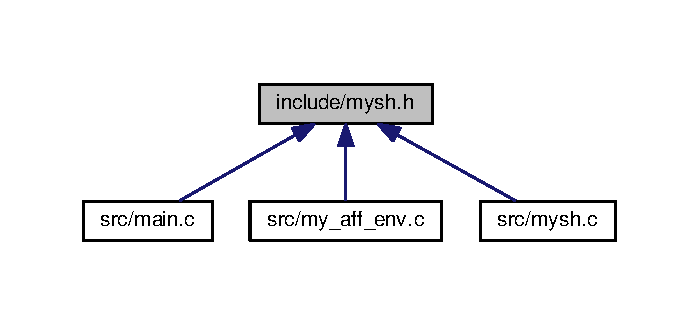
\includegraphics[width=336pt]{mysh_8h__dep__incl}
\end{center}
\end{figure}
\subsection*{Data Structures}
\begin{DoxyCompactItemize}
\item 
struct \hyperlink{structs__ptrtab}{s\+\_\+ptrtab}
\end{DoxyCompactItemize}
\subsection*{Typedefs}
\begin{DoxyCompactItemize}
\item 
typedef struct \hyperlink{structs__ptrtab}{s\+\_\+ptrtab} \hyperlink{mysh_8h_a4899c523e923a9c28fb835488907c6f7}{t\+\_\+ptrtab}
\end{DoxyCompactItemize}
\subsection*{Functions}
\begin{DoxyCompactItemize}
\item 
char $\ast$ \hyperlink{mysh_8h_aa36259f17fd04d9decba71955aedeb45}{get\+\_\+next\+\_\+line} (const int fd)
\item 
void \hyperlink{mysh_8h_a12eed0970f97b5ae8dc85cce79a44827}{my\+\_\+prompt} ()
\item 
int \hyperlink{mysh_8h_a92bb32d622719b834371dfdacdb56d09}{minishell1} (char $\ast$$\ast$env)
\item 
void \hyperlink{mysh_8h_ad8bca16f1928a1facff1dbffe5118774}{my\+\_\+aff\+\_\+env} (char $\ast$$\ast$env)
\end{DoxyCompactItemize}


\subsection{Typedef Documentation}
\hypertarget{mysh_8h_a4899c523e923a9c28fb835488907c6f7}{\index{mysh.\+h@{mysh.\+h}!t\+\_\+ptrtab@{t\+\_\+ptrtab}}
\index{t\+\_\+ptrtab@{t\+\_\+ptrtab}!mysh.\+h@{mysh.\+h}}
\subsubsection[{t\+\_\+ptrtab}]{\setlength{\rightskip}{0pt plus 5cm}typedef struct {\bf s\+\_\+ptrtab}		 {\bf t\+\_\+ptrtab}}}\label{mysh_8h_a4899c523e923a9c28fb835488907c6f7}


\subsection{Function Documentation}
\hypertarget{mysh_8h_aa36259f17fd04d9decba71955aedeb45}{\index{mysh.\+h@{mysh.\+h}!get\+\_\+next\+\_\+line@{get\+\_\+next\+\_\+line}}
\index{get\+\_\+next\+\_\+line@{get\+\_\+next\+\_\+line}!mysh.\+h@{mysh.\+h}}
\subsubsection[{get\+\_\+next\+\_\+line}]{\setlength{\rightskip}{0pt plus 5cm}char$\ast$ get\+\_\+next\+\_\+line (
\begin{DoxyParamCaption}
\item[{const int}]{fd}
\end{DoxyParamCaption}
)}}\label{mysh_8h_aa36259f17fd04d9decba71955aedeb45}


Definition at line 81 of file get\+\_\+next\+\_\+line.\+c.

\hypertarget{mysh_8h_a92bb32d622719b834371dfdacdb56d09}{\index{mysh.\+h@{mysh.\+h}!minishell1@{minishell1}}
\index{minishell1@{minishell1}!mysh.\+h@{mysh.\+h}}
\subsubsection[{minishell1}]{\setlength{\rightskip}{0pt plus 5cm}int minishell1 (
\begin{DoxyParamCaption}
\item[{char $\ast$$\ast$}]{env}
\end{DoxyParamCaption}
)}}\label{mysh_8h_a92bb32d622719b834371dfdacdb56d09}


Definition at line 217 of file mysh.\+c.

\hypertarget{mysh_8h_ad8bca16f1928a1facff1dbffe5118774}{\index{mysh.\+h@{mysh.\+h}!my\+\_\+aff\+\_\+env@{my\+\_\+aff\+\_\+env}}
\index{my\+\_\+aff\+\_\+env@{my\+\_\+aff\+\_\+env}!mysh.\+h@{mysh.\+h}}
\subsubsection[{my\+\_\+aff\+\_\+env}]{\setlength{\rightskip}{0pt plus 5cm}void my\+\_\+aff\+\_\+env (
\begin{DoxyParamCaption}
\item[{char $\ast$$\ast$}]{env}
\end{DoxyParamCaption}
)}}\label{mysh_8h_ad8bca16f1928a1facff1dbffe5118774}


Definition at line 15 of file my\+\_\+aff\+\_\+env.\+c.

\hypertarget{mysh_8h_a12eed0970f97b5ae8dc85cce79a44827}{\index{mysh.\+h@{mysh.\+h}!my\+\_\+prompt@{my\+\_\+prompt}}
\index{my\+\_\+prompt@{my\+\_\+prompt}!mysh.\+h@{mysh.\+h}}
\subsubsection[{my\+\_\+prompt}]{\setlength{\rightskip}{0pt plus 5cm}void my\+\_\+prompt (
\begin{DoxyParamCaption}
{}
\end{DoxyParamCaption}
)}}\label{mysh_8h_a12eed0970f97b5ae8dc85cce79a44827}


Definition at line 233 of file mysh.\+c.


\hypertarget{case__l_8c}{\section{lib/my/src/printf/case\+\_\+l.c File Reference}
\label{case__l_8c}\index{lib/my/src/printf/case\+\_\+l.\+c@{lib/my/src/printf/case\+\_\+l.\+c}}
}
{\ttfamily \#include \char`\"{}my.\+h\char`\"{}}\\*
Include dependency graph for case\+\_\+l.\+c\+:
\nopagebreak
\begin{figure}[H]
\begin{center}
\leavevmode
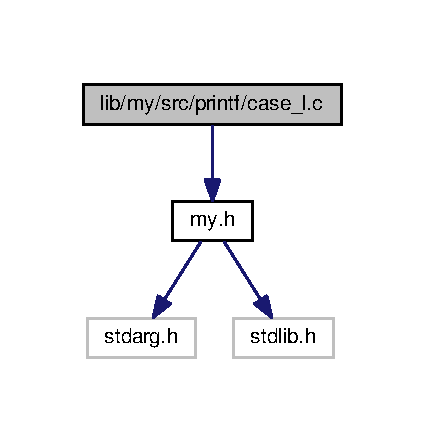
\includegraphics[width=204pt]{case__l_8c__incl}
\end{center}
\end{figure}
\subsection*{Functions}
\begin{DoxyCompactItemize}
\item 
int \hyperlink{case__l_8c_a4861f05079aaf8e8313344b16751a0a6}{case\+\_\+l} (void $\ast$argv, \hyperlink{my_8h_a648ad484eb5d7e8f5d781c45b20f874f}{t\+\_\+index} $\ast$s, const char $\ast$format, const \hyperlink{my_8h_ac25c8b585b5df2bbafd4bdceafa17eb4}{t\+\_\+struc} $\ast$tab)
\end{DoxyCompactItemize}


\subsection{Function Documentation}
\hypertarget{case__l_8c_a4861f05079aaf8e8313344b16751a0a6}{\index{case\+\_\+l.\+c@{case\+\_\+l.\+c}!case\+\_\+l@{case\+\_\+l}}
\index{case\+\_\+l@{case\+\_\+l}!case\+\_\+l.\+c@{case\+\_\+l.\+c}}
\subsubsection[{case\+\_\+l}]{\setlength{\rightskip}{0pt plus 5cm}int case\+\_\+l (
\begin{DoxyParamCaption}
\item[{void $\ast$}]{argv, }
\item[{{\bf t\+\_\+index} $\ast$}]{s, }
\item[{const char $\ast$}]{format, }
\item[{const {\bf t\+\_\+struc} $\ast$}]{tab}
\end{DoxyParamCaption}
)}}\label{case__l_8c_a4861f05079aaf8e8313344b16751a0a6}


Definition at line 13 of file case\+\_\+l.\+c.


\hypertarget{case__printf__aff_8c}{\section{lib/my/src/printf/case\+\_\+printf\+\_\+aff.c File Reference}
\label{case__printf__aff_8c}\index{lib/my/src/printf/case\+\_\+printf\+\_\+aff.\+c@{lib/my/src/printf/case\+\_\+printf\+\_\+aff.\+c}}
}
{\ttfamily \#include \char`\"{}my.\+h\char`\"{}}\\*
Include dependency graph for case\+\_\+printf\+\_\+aff.\+c\+:
\nopagebreak
\begin{figure}[H]
\begin{center}
\leavevmode
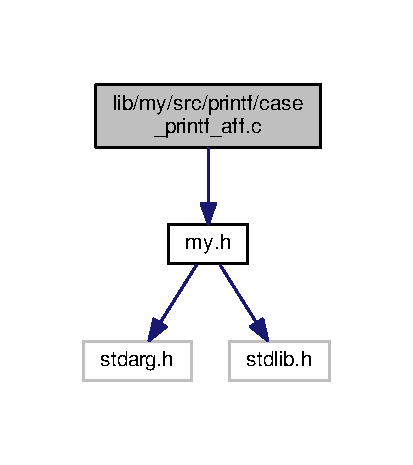
\includegraphics[width=198pt]{case__printf__aff_8c__incl}
\end{center}
\end{figure}
\subsection*{Functions}
\begin{DoxyCompactItemize}
\item 
int \hyperlink{case__printf__aff_8c_a210d12a636371bbb0f25115451e88ea6}{s\+\_\+putstr} (void $\ast$argv, \hyperlink{my_8h_a648ad484eb5d7e8f5d781c45b20f874f}{t\+\_\+index} $\ast$s, const char $\ast$format, const \hyperlink{my_8h_ac25c8b585b5df2bbafd4bdceafa17eb4}{t\+\_\+struc} $\ast$tab)
\item 
int \hyperlink{case__printf__aff_8c_a2ca0365009481f7563e0f8c08cf0e0c9}{case\+\_\+p} (void $\ast$argv, \hyperlink{my_8h_a648ad484eb5d7e8f5d781c45b20f874f}{t\+\_\+index} $\ast$s, const char $\ast$format, const \hyperlink{my_8h_ac25c8b585b5df2bbafd4bdceafa17eb4}{t\+\_\+struc} $\ast$tab)
\item 
int \hyperlink{case__printf__aff_8c_a500cb9fd540fc8337d1bdebb9df56439}{case\+\_\+x} (void $\ast$argv, \hyperlink{my_8h_a648ad484eb5d7e8f5d781c45b20f874f}{t\+\_\+index} $\ast$s, const char $\ast$format, const \hyperlink{my_8h_ac25c8b585b5df2bbafd4bdceafa17eb4}{t\+\_\+struc} $\ast$tab)
\item 
int \hyperlink{case__printf__aff_8c_a3535db665dd6c72c791567112877de4a}{case\+\_\+c} (void $\ast$argv, \hyperlink{my_8h_a648ad484eb5d7e8f5d781c45b20f874f}{t\+\_\+index} $\ast$s, const char $\ast$format, const \hyperlink{my_8h_ac25c8b585b5df2bbafd4bdceafa17eb4}{t\+\_\+struc} $\ast$tab)
\item 
int \hyperlink{case__printf__aff_8c_a91c72293ad0ca640b91b6178fed1ebb2}{case\+\_\+s} (void $\ast$argv, \hyperlink{my_8h_a648ad484eb5d7e8f5d781c45b20f874f}{t\+\_\+index} $\ast$s, const char $\ast$format, const \hyperlink{my_8h_ac25c8b585b5df2bbafd4bdceafa17eb4}{t\+\_\+struc} $\ast$tab)
\end{DoxyCompactItemize}


\subsection{Function Documentation}
\hypertarget{case__printf__aff_8c_a3535db665dd6c72c791567112877de4a}{\index{case\+\_\+printf\+\_\+aff.\+c@{case\+\_\+printf\+\_\+aff.\+c}!case\+\_\+c@{case\+\_\+c}}
\index{case\+\_\+c@{case\+\_\+c}!case\+\_\+printf\+\_\+aff.\+c@{case\+\_\+printf\+\_\+aff.\+c}}
\subsubsection[{case\+\_\+c}]{\setlength{\rightskip}{0pt plus 5cm}int case\+\_\+c (
\begin{DoxyParamCaption}
\item[{void $\ast$}]{argv, }
\item[{{\bf t\+\_\+index} $\ast$}]{s, }
\item[{const char $\ast$}]{format, }
\item[{const {\bf t\+\_\+struc} $\ast$}]{tab}
\end{DoxyParamCaption}
)}}\label{case__printf__aff_8c_a3535db665dd6c72c791567112877de4a}


Definition at line 66 of file case\+\_\+printf\+\_\+aff.\+c.

\hypertarget{case__printf__aff_8c_a2ca0365009481f7563e0f8c08cf0e0c9}{\index{case\+\_\+printf\+\_\+aff.\+c@{case\+\_\+printf\+\_\+aff.\+c}!case\+\_\+p@{case\+\_\+p}}
\index{case\+\_\+p@{case\+\_\+p}!case\+\_\+printf\+\_\+aff.\+c@{case\+\_\+printf\+\_\+aff.\+c}}
\subsubsection[{case\+\_\+p}]{\setlength{\rightskip}{0pt plus 5cm}int case\+\_\+p (
\begin{DoxyParamCaption}
\item[{void $\ast$}]{argv, }
\item[{{\bf t\+\_\+index} $\ast$}]{s, }
\item[{const char $\ast$}]{format, }
\item[{const {\bf t\+\_\+struc} $\ast$}]{tab}
\end{DoxyParamCaption}
)}}\label{case__printf__aff_8c_a2ca0365009481f7563e0f8c08cf0e0c9}


Definition at line 35 of file case\+\_\+printf\+\_\+aff.\+c.

\hypertarget{case__printf__aff_8c_a91c72293ad0ca640b91b6178fed1ebb2}{\index{case\+\_\+printf\+\_\+aff.\+c@{case\+\_\+printf\+\_\+aff.\+c}!case\+\_\+s@{case\+\_\+s}}
\index{case\+\_\+s@{case\+\_\+s}!case\+\_\+printf\+\_\+aff.\+c@{case\+\_\+printf\+\_\+aff.\+c}}
\subsubsection[{case\+\_\+s}]{\setlength{\rightskip}{0pt plus 5cm}int case\+\_\+s (
\begin{DoxyParamCaption}
\item[{void $\ast$}]{argv, }
\item[{{\bf t\+\_\+index} $\ast$}]{s, }
\item[{const char $\ast$}]{format, }
\item[{const {\bf t\+\_\+struc} $\ast$}]{tab}
\end{DoxyParamCaption}
)}}\label{case__printf__aff_8c_a91c72293ad0ca640b91b6178fed1ebb2}


Definition at line 79 of file case\+\_\+printf\+\_\+aff.\+c.

\hypertarget{case__printf__aff_8c_a500cb9fd540fc8337d1bdebb9df56439}{\index{case\+\_\+printf\+\_\+aff.\+c@{case\+\_\+printf\+\_\+aff.\+c}!case\+\_\+x@{case\+\_\+x}}
\index{case\+\_\+x@{case\+\_\+x}!case\+\_\+printf\+\_\+aff.\+c@{case\+\_\+printf\+\_\+aff.\+c}}
\subsubsection[{case\+\_\+x}]{\setlength{\rightskip}{0pt plus 5cm}int case\+\_\+x (
\begin{DoxyParamCaption}
\item[{void $\ast$}]{argv, }
\item[{{\bf t\+\_\+index} $\ast$}]{s, }
\item[{const char $\ast$}]{format, }
\item[{const {\bf t\+\_\+struc} $\ast$}]{tab}
\end{DoxyParamCaption}
)}}\label{case__printf__aff_8c_a500cb9fd540fc8337d1bdebb9df56439}


Definition at line 49 of file case\+\_\+printf\+\_\+aff.\+c.

\hypertarget{case__printf__aff_8c_a210d12a636371bbb0f25115451e88ea6}{\index{case\+\_\+printf\+\_\+aff.\+c@{case\+\_\+printf\+\_\+aff.\+c}!s\+\_\+putstr@{s\+\_\+putstr}}
\index{s\+\_\+putstr@{s\+\_\+putstr}!case\+\_\+printf\+\_\+aff.\+c@{case\+\_\+printf\+\_\+aff.\+c}}
\subsubsection[{s\+\_\+putstr}]{\setlength{\rightskip}{0pt plus 5cm}int s\+\_\+putstr (
\begin{DoxyParamCaption}
\item[{void $\ast$}]{argv, }
\item[{{\bf t\+\_\+index} $\ast$}]{s, }
\item[{const char $\ast$}]{format, }
\item[{const {\bf t\+\_\+struc} $\ast$}]{tab}
\end{DoxyParamCaption}
)}}\label{case__printf__aff_8c_a210d12a636371bbb0f25115451e88ea6}


Definition at line 13 of file case\+\_\+printf\+\_\+aff.\+c.


\hypertarget{case__printf__convert_8c}{\section{lib/my/src/printf/case\+\_\+printf\+\_\+convert.c File Reference}
\label{case__printf__convert_8c}\index{lib/my/src/printf/case\+\_\+printf\+\_\+convert.\+c@{lib/my/src/printf/case\+\_\+printf\+\_\+convert.\+c}}
}
{\ttfamily \#include \char`\"{}my.\+h\char`\"{}}\\*
Include dependency graph for case\+\_\+printf\+\_\+convert.\+c\+:
\nopagebreak
\begin{figure}[H]
\begin{center}
\leavevmode
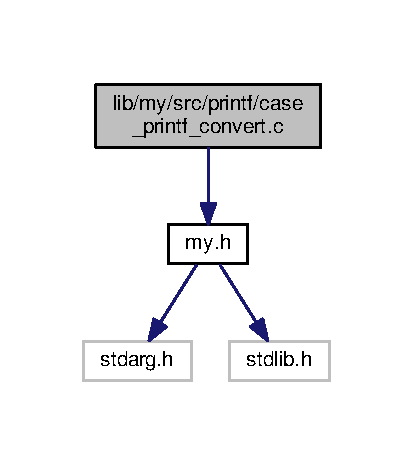
\includegraphics[width=198pt]{case__printf__convert_8c__incl}
\end{center}
\end{figure}
\subsection*{Functions}
\begin{DoxyCompactItemize}
\item 
int \hyperlink{case__printf__convert_8c_a83a21528a9e6f2461dba942d6892c1a8}{case\+\_\+pres} (void $\ast$argv, \hyperlink{my_8h_a648ad484eb5d7e8f5d781c45b20f874f}{t\+\_\+index} $\ast$s, const char $\ast$format, const \hyperlink{my_8h_ac25c8b585b5df2bbafd4bdceafa17eb4}{t\+\_\+struc} $\ast$tab)
\item 
int \hyperlink{case__printf__convert_8c_ab13cbc229e8177d316dd3d9d88cdb567}{case\+\_\+sharp2} (\hyperlink{my_8h_a648ad484eb5d7e8f5d781c45b20f874f}{t\+\_\+index} $\ast$s, const char $\ast$format, int i, const \hyperlink{my_8h_ac25c8b585b5df2bbafd4bdceafa17eb4}{t\+\_\+struc} $\ast$tab)
\item 
int \hyperlink{case__printf__convert_8c_abaafbf096a795ff378896ed44c85bf0e}{case\+\_\+sharp} (void $\ast$argv, \hyperlink{my_8h_a648ad484eb5d7e8f5d781c45b20f874f}{t\+\_\+index} $\ast$s, const char $\ast$format, const \hyperlink{my_8h_ac25c8b585b5df2bbafd4bdceafa17eb4}{t\+\_\+struc} $\ast$tab)
\item 
int \hyperlink{case__printf__convert_8c_a013d463656e55e0618a6e1f4d937168a}{case\+\_\+zero} (void $\ast$argv, \hyperlink{my_8h_a648ad484eb5d7e8f5d781c45b20f874f}{t\+\_\+index} $\ast$s, const char $\ast$format, const \hyperlink{my_8h_ac25c8b585b5df2bbafd4bdceafa17eb4}{t\+\_\+struc} $\ast$tab)
\end{DoxyCompactItemize}


\subsection{Function Documentation}
\hypertarget{case__printf__convert_8c_a83a21528a9e6f2461dba942d6892c1a8}{\index{case\+\_\+printf\+\_\+convert.\+c@{case\+\_\+printf\+\_\+convert.\+c}!case\+\_\+pres@{case\+\_\+pres}}
\index{case\+\_\+pres@{case\+\_\+pres}!case\+\_\+printf\+\_\+convert.\+c@{case\+\_\+printf\+\_\+convert.\+c}}
\subsubsection[{case\+\_\+pres}]{\setlength{\rightskip}{0pt plus 5cm}int case\+\_\+pres (
\begin{DoxyParamCaption}
\item[{void $\ast$}]{argv, }
\item[{{\bf t\+\_\+index} $\ast$}]{s, }
\item[{const char $\ast$}]{format, }
\item[{const {\bf t\+\_\+struc} $\ast$}]{tab}
\end{DoxyParamCaption}
)}}\label{case__printf__convert_8c_a83a21528a9e6f2461dba942d6892c1a8}


Definition at line 13 of file case\+\_\+printf\+\_\+convert.\+c.

\hypertarget{case__printf__convert_8c_abaafbf096a795ff378896ed44c85bf0e}{\index{case\+\_\+printf\+\_\+convert.\+c@{case\+\_\+printf\+\_\+convert.\+c}!case\+\_\+sharp@{case\+\_\+sharp}}
\index{case\+\_\+sharp@{case\+\_\+sharp}!case\+\_\+printf\+\_\+convert.\+c@{case\+\_\+printf\+\_\+convert.\+c}}
\subsubsection[{case\+\_\+sharp}]{\setlength{\rightskip}{0pt plus 5cm}int case\+\_\+sharp (
\begin{DoxyParamCaption}
\item[{void $\ast$}]{argv, }
\item[{{\bf t\+\_\+index} $\ast$}]{s, }
\item[{const char $\ast$}]{format, }
\item[{const {\bf t\+\_\+struc} $\ast$}]{tab}
\end{DoxyParamCaption}
)}}\label{case__printf__convert_8c_abaafbf096a795ff378896ed44c85bf0e}


Definition at line 42 of file case\+\_\+printf\+\_\+convert.\+c.

\hypertarget{case__printf__convert_8c_ab13cbc229e8177d316dd3d9d88cdb567}{\index{case\+\_\+printf\+\_\+convert.\+c@{case\+\_\+printf\+\_\+convert.\+c}!case\+\_\+sharp2@{case\+\_\+sharp2}}
\index{case\+\_\+sharp2@{case\+\_\+sharp2}!case\+\_\+printf\+\_\+convert.\+c@{case\+\_\+printf\+\_\+convert.\+c}}
\subsubsection[{case\+\_\+sharp2}]{\setlength{\rightskip}{0pt plus 5cm}int case\+\_\+sharp2 (
\begin{DoxyParamCaption}
\item[{{\bf t\+\_\+index} $\ast$}]{s, }
\item[{const char $\ast$}]{format, }
\item[{int}]{i, }
\item[{const {\bf t\+\_\+struc} $\ast$}]{tab}
\end{DoxyParamCaption}
)}}\label{case__printf__convert_8c_ab13cbc229e8177d316dd3d9d88cdb567}


Definition at line 24 of file case\+\_\+printf\+\_\+convert.\+c.

\hypertarget{case__printf__convert_8c_a013d463656e55e0618a6e1f4d937168a}{\index{case\+\_\+printf\+\_\+convert.\+c@{case\+\_\+printf\+\_\+convert.\+c}!case\+\_\+zero@{case\+\_\+zero}}
\index{case\+\_\+zero@{case\+\_\+zero}!case\+\_\+printf\+\_\+convert.\+c@{case\+\_\+printf\+\_\+convert.\+c}}
\subsubsection[{case\+\_\+zero}]{\setlength{\rightskip}{0pt plus 5cm}int case\+\_\+zero (
\begin{DoxyParamCaption}
\item[{void $\ast$}]{argv, }
\item[{{\bf t\+\_\+index} $\ast$}]{s, }
\item[{const char $\ast$}]{format, }
\item[{const {\bf t\+\_\+struc} $\ast$}]{tab}
\end{DoxyParamCaption}
)}}\label{case__printf__convert_8c_a013d463656e55e0618a6e1f4d937168a}


Definition at line 63 of file case\+\_\+printf\+\_\+convert.\+c.


\hypertarget{case__printf__nb_8c}{\section{lib/my/src/printf/case\+\_\+printf\+\_\+nb.c File Reference}
\label{case__printf__nb_8c}\index{lib/my/src/printf/case\+\_\+printf\+\_\+nb.\+c@{lib/my/src/printf/case\+\_\+printf\+\_\+nb.\+c}}
}
{\ttfamily \#include \char`\"{}my.\+h\char`\"{}}\\*
Include dependency graph for case\+\_\+printf\+\_\+nb.\+c\+:
\nopagebreak
\begin{figure}[H]
\begin{center}
\leavevmode
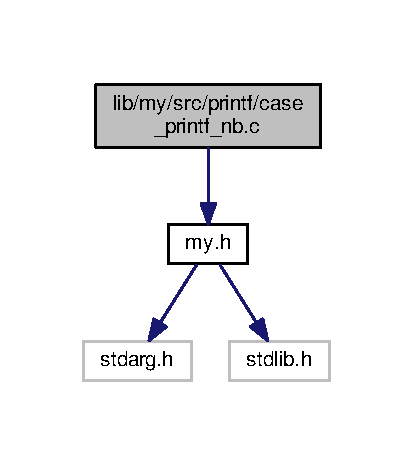
\includegraphics[width=198pt]{case__printf__nb_8c__incl}
\end{center}
\end{figure}
\subsection*{Functions}
\begin{DoxyCompactItemize}
\item 
int \hyperlink{case__printf__nb_8c_a68fff7b819caa6ed822d928e544b294c}{case\+\_\+b} (void $\ast$argv, \hyperlink{my_8h_a648ad484eb5d7e8f5d781c45b20f874f}{t\+\_\+index} $\ast$s, const char $\ast$format, const \hyperlink{my_8h_ac25c8b585b5df2bbafd4bdceafa17eb4}{t\+\_\+struc} $\ast$tab)
\item 
int \hyperlink{case__printf__nb_8c_af87d61ca079d23141a1d403abdb3bd2d}{case\+\_\+di} (void $\ast$argv, \hyperlink{my_8h_a648ad484eb5d7e8f5d781c45b20f874f}{t\+\_\+index} $\ast$s, const char $\ast$format, const \hyperlink{my_8h_ac25c8b585b5df2bbafd4bdceafa17eb4}{t\+\_\+struc} $\ast$tab)
\item 
int \hyperlink{case__printf__nb_8c_a752193ef66373cc419bfabdcc7850b49}{case\+\_\+o} (void $\ast$argv, \hyperlink{my_8h_a648ad484eb5d7e8f5d781c45b20f874f}{t\+\_\+index} $\ast$s, const char $\ast$format, const \hyperlink{my_8h_ac25c8b585b5df2bbafd4bdceafa17eb4}{t\+\_\+struc} $\ast$tab)
\item 
int \hyperlink{case__printf__nb_8c_a4333d447daeb94aa2c59468dd2dee929}{x\+\_\+case} (void $\ast$argv, \hyperlink{my_8h_a648ad484eb5d7e8f5d781c45b20f874f}{t\+\_\+index} $\ast$s, const char $\ast$format, const \hyperlink{my_8h_ac25c8b585b5df2bbafd4bdceafa17eb4}{t\+\_\+struc} $\ast$tab)
\item 
int \hyperlink{case__printf__nb_8c_ae7a0d4d53622aae2844818b9b55c6a48}{case\+\_\+u} (void $\ast$argv, \hyperlink{my_8h_a648ad484eb5d7e8f5d781c45b20f874f}{t\+\_\+index} $\ast$s, const char $\ast$format, const \hyperlink{my_8h_ac25c8b585b5df2bbafd4bdceafa17eb4}{t\+\_\+struc} $\ast$tab)
\end{DoxyCompactItemize}


\subsection{Function Documentation}
\hypertarget{case__printf__nb_8c_a68fff7b819caa6ed822d928e544b294c}{\index{case\+\_\+printf\+\_\+nb.\+c@{case\+\_\+printf\+\_\+nb.\+c}!case\+\_\+b@{case\+\_\+b}}
\index{case\+\_\+b@{case\+\_\+b}!case\+\_\+printf\+\_\+nb.\+c@{case\+\_\+printf\+\_\+nb.\+c}}
\subsubsection[{case\+\_\+b}]{\setlength{\rightskip}{0pt plus 5cm}int case\+\_\+b (
\begin{DoxyParamCaption}
\item[{void $\ast$}]{argv, }
\item[{{\bf t\+\_\+index} $\ast$}]{s, }
\item[{const char $\ast$}]{format, }
\item[{const {\bf t\+\_\+struc} $\ast$}]{tab}
\end{DoxyParamCaption}
)}}\label{case__printf__nb_8c_a68fff7b819caa6ed822d928e544b294c}


Definition at line 13 of file case\+\_\+printf\+\_\+nb.\+c.

\hypertarget{case__printf__nb_8c_af87d61ca079d23141a1d403abdb3bd2d}{\index{case\+\_\+printf\+\_\+nb.\+c@{case\+\_\+printf\+\_\+nb.\+c}!case\+\_\+di@{case\+\_\+di}}
\index{case\+\_\+di@{case\+\_\+di}!case\+\_\+printf\+\_\+nb.\+c@{case\+\_\+printf\+\_\+nb.\+c}}
\subsubsection[{case\+\_\+di}]{\setlength{\rightskip}{0pt plus 5cm}int case\+\_\+di (
\begin{DoxyParamCaption}
\item[{void $\ast$}]{argv, }
\item[{{\bf t\+\_\+index} $\ast$}]{s, }
\item[{const char $\ast$}]{format, }
\item[{const {\bf t\+\_\+struc} $\ast$}]{tab}
\end{DoxyParamCaption}
)}}\label{case__printf__nb_8c_af87d61ca079d23141a1d403abdb3bd2d}


Definition at line 27 of file case\+\_\+printf\+\_\+nb.\+c.

\hypertarget{case__printf__nb_8c_a752193ef66373cc419bfabdcc7850b49}{\index{case\+\_\+printf\+\_\+nb.\+c@{case\+\_\+printf\+\_\+nb.\+c}!case\+\_\+o@{case\+\_\+o}}
\index{case\+\_\+o@{case\+\_\+o}!case\+\_\+printf\+\_\+nb.\+c@{case\+\_\+printf\+\_\+nb.\+c}}
\subsubsection[{case\+\_\+o}]{\setlength{\rightskip}{0pt plus 5cm}int case\+\_\+o (
\begin{DoxyParamCaption}
\item[{void $\ast$}]{argv, }
\item[{{\bf t\+\_\+index} $\ast$}]{s, }
\item[{const char $\ast$}]{format, }
\item[{const {\bf t\+\_\+struc} $\ast$}]{tab}
\end{DoxyParamCaption}
)}}\label{case__printf__nb_8c_a752193ef66373cc419bfabdcc7850b49}


Definition at line 44 of file case\+\_\+printf\+\_\+nb.\+c.

\hypertarget{case__printf__nb_8c_ae7a0d4d53622aae2844818b9b55c6a48}{\index{case\+\_\+printf\+\_\+nb.\+c@{case\+\_\+printf\+\_\+nb.\+c}!case\+\_\+u@{case\+\_\+u}}
\index{case\+\_\+u@{case\+\_\+u}!case\+\_\+printf\+\_\+nb.\+c@{case\+\_\+printf\+\_\+nb.\+c}}
\subsubsection[{case\+\_\+u}]{\setlength{\rightskip}{0pt plus 5cm}int case\+\_\+u (
\begin{DoxyParamCaption}
\item[{void $\ast$}]{argv, }
\item[{{\bf t\+\_\+index} $\ast$}]{s, }
\item[{const char $\ast$}]{format, }
\item[{const {\bf t\+\_\+struc} $\ast$}]{tab}
\end{DoxyParamCaption}
)}}\label{case__printf__nb_8c_ae7a0d4d53622aae2844818b9b55c6a48}


Definition at line 79 of file case\+\_\+printf\+\_\+nb.\+c.

\hypertarget{case__printf__nb_8c_a4333d447daeb94aa2c59468dd2dee929}{\index{case\+\_\+printf\+\_\+nb.\+c@{case\+\_\+printf\+\_\+nb.\+c}!x\+\_\+case@{x\+\_\+case}}
\index{x\+\_\+case@{x\+\_\+case}!case\+\_\+printf\+\_\+nb.\+c@{case\+\_\+printf\+\_\+nb.\+c}}
\subsubsection[{x\+\_\+case}]{\setlength{\rightskip}{0pt plus 5cm}int x\+\_\+case (
\begin{DoxyParamCaption}
\item[{void $\ast$}]{argv, }
\item[{{\bf t\+\_\+index} $\ast$}]{s, }
\item[{const char $\ast$}]{format, }
\item[{const {\bf t\+\_\+struc} $\ast$}]{tab}
\end{DoxyParamCaption}
)}}\label{case__printf__nb_8c_a4333d447daeb94aa2c59468dd2dee929}


Definition at line 62 of file case\+\_\+printf\+\_\+nb.\+c.


\hypertarget{convert__base__16_8c}{\section{lib/my/src/printf/convert\+\_\+base\+\_\+16.c File Reference}
\label{convert__base__16_8c}\index{lib/my/src/printf/convert\+\_\+base\+\_\+16.\+c@{lib/my/src/printf/convert\+\_\+base\+\_\+16.\+c}}
}
{\ttfamily \#include \char`\"{}my.\+h\char`\"{}}\\*
Include dependency graph for convert\+\_\+base\+\_\+16.\+c\+:
\nopagebreak
\begin{figure}[H]
\begin{center}
\leavevmode
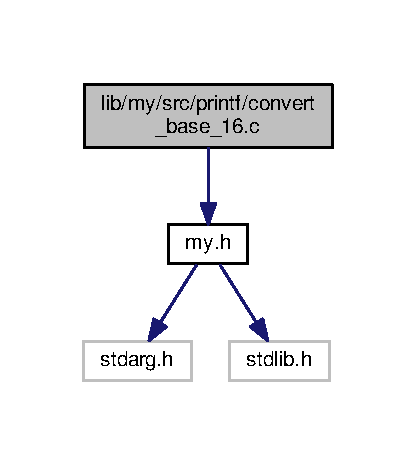
\includegraphics[width=200pt]{convert__base__16_8c__incl}
\end{center}
\end{figure}
\subsection*{Functions}
\begin{DoxyCompactItemize}
\item 
int \hyperlink{convert__base__16_8c_ac7e9bd08d068851e31a5b6d408004638}{my\+\_\+strlen} (char $\ast$str)
\item 
int \hyperlink{convert__base__16_8c_aa6df05dfcbd54dc062af6e56215f656f}{my\+\_\+rev\+\_\+int\+\_\+tab\+\_\+long} (char $\ast$tab, long i)
\item 
void \hyperlink{convert__base__16_8c_ab228b9450ae618a46ca62d2b1809574f}{my\+\_\+rev\+\_\+int\+\_\+tab\+\_\+un} (char $\ast$tab, long i)
\item 
void \hyperlink{convert__base__16_8c_a19c537e65b212d78f6088c53687fa546}{my\+\_\+rev\+\_\+int\+\_\+tab} (int $\ast$tab, int i)
\end{DoxyCompactItemize}


\subsection{Function Documentation}
\hypertarget{convert__base__16_8c_a19c537e65b212d78f6088c53687fa546}{\index{convert\+\_\+base\+\_\+16.\+c@{convert\+\_\+base\+\_\+16.\+c}!my\+\_\+rev\+\_\+int\+\_\+tab@{my\+\_\+rev\+\_\+int\+\_\+tab}}
\index{my\+\_\+rev\+\_\+int\+\_\+tab@{my\+\_\+rev\+\_\+int\+\_\+tab}!convert\+\_\+base\+\_\+16.\+c@{convert\+\_\+base\+\_\+16.\+c}}
\subsubsection[{my\+\_\+rev\+\_\+int\+\_\+tab}]{\setlength{\rightskip}{0pt plus 5cm}void my\+\_\+rev\+\_\+int\+\_\+tab (
\begin{DoxyParamCaption}
\item[{int $\ast$}]{tab, }
\item[{int}]{i}
\end{DoxyParamCaption}
)}}\label{convert__base__16_8c_a19c537e65b212d78f6088c53687fa546}


Definition at line 54 of file convert\+\_\+base\+\_\+16.\+c.

\hypertarget{convert__base__16_8c_aa6df05dfcbd54dc062af6e56215f656f}{\index{convert\+\_\+base\+\_\+16.\+c@{convert\+\_\+base\+\_\+16.\+c}!my\+\_\+rev\+\_\+int\+\_\+tab\+\_\+long@{my\+\_\+rev\+\_\+int\+\_\+tab\+\_\+long}}
\index{my\+\_\+rev\+\_\+int\+\_\+tab\+\_\+long@{my\+\_\+rev\+\_\+int\+\_\+tab\+\_\+long}!convert\+\_\+base\+\_\+16.\+c@{convert\+\_\+base\+\_\+16.\+c}}
\subsubsection[{my\+\_\+rev\+\_\+int\+\_\+tab\+\_\+long}]{\setlength{\rightskip}{0pt plus 5cm}int my\+\_\+rev\+\_\+int\+\_\+tab\+\_\+long (
\begin{DoxyParamCaption}
\item[{char $\ast$}]{tab, }
\item[{long}]{i}
\end{DoxyParamCaption}
)}}\label{convert__base__16_8c_aa6df05dfcbd54dc062af6e56215f656f}


Definition at line 23 of file convert\+\_\+base\+\_\+16.\+c.

\hypertarget{convert__base__16_8c_ab228b9450ae618a46ca62d2b1809574f}{\index{convert\+\_\+base\+\_\+16.\+c@{convert\+\_\+base\+\_\+16.\+c}!my\+\_\+rev\+\_\+int\+\_\+tab\+\_\+un@{my\+\_\+rev\+\_\+int\+\_\+tab\+\_\+un}}
\index{my\+\_\+rev\+\_\+int\+\_\+tab\+\_\+un@{my\+\_\+rev\+\_\+int\+\_\+tab\+\_\+un}!convert\+\_\+base\+\_\+16.\+c@{convert\+\_\+base\+\_\+16.\+c}}
\subsubsection[{my\+\_\+rev\+\_\+int\+\_\+tab\+\_\+un}]{\setlength{\rightskip}{0pt plus 5cm}void my\+\_\+rev\+\_\+int\+\_\+tab\+\_\+un (
\begin{DoxyParamCaption}
\item[{char $\ast$}]{tab, }
\item[{long}]{i}
\end{DoxyParamCaption}
)}}\label{convert__base__16_8c_ab228b9450ae618a46ca62d2b1809574f}


Definition at line 44 of file convert\+\_\+base\+\_\+16.\+c.

\hypertarget{convert__base__16_8c_ac7e9bd08d068851e31a5b6d408004638}{\index{convert\+\_\+base\+\_\+16.\+c@{convert\+\_\+base\+\_\+16.\+c}!my\+\_\+strlen@{my\+\_\+strlen}}
\index{my\+\_\+strlen@{my\+\_\+strlen}!convert\+\_\+base\+\_\+16.\+c@{convert\+\_\+base\+\_\+16.\+c}}
\subsubsection[{my\+\_\+strlen}]{\setlength{\rightskip}{0pt plus 5cm}int my\+\_\+strlen (
\begin{DoxyParamCaption}
\item[{char $\ast$}]{str}
\end{DoxyParamCaption}
)}}\label{convert__base__16_8c_ac7e9bd08d068851e31a5b6d408004638}


Definition at line 13 of file convert\+\_\+base\+\_\+16.\+c.


\hypertarget{convert__base__8_8c}{\section{lib/my/src/printf/convert\+\_\+base\+\_\+8.c File Reference}
\label{convert__base__8_8c}\index{lib/my/src/printf/convert\+\_\+base\+\_\+8.\+c@{lib/my/src/printf/convert\+\_\+base\+\_\+8.\+c}}
}
{\ttfamily \#include $<$stdlib.\+h$>$}\\*
{\ttfamily \#include \char`\"{}my.\+h\char`\"{}}\\*
Include dependency graph for convert\+\_\+base\+\_\+8.\+c\+:
\nopagebreak
\begin{figure}[H]
\begin{center}
\leavevmode
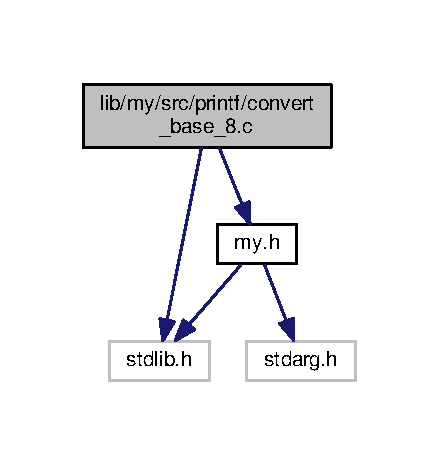
\includegraphics[width=211pt]{convert__base__8_8c__incl}
\end{center}
\end{figure}
\subsection*{Functions}
\begin{DoxyCompactItemize}
\item 
void \hyperlink{convert__base__8_8c_a1d732a4c44f1469c1fb09eab715773ec}{my\+\_\+rev\+\_\+unint\+\_\+tab} (unsigned int $\ast$tab, int i)
\item 
void \hyperlink{convert__base__8_8c_afc785712bfc7354145b34cfbc3a33631}{my\+\_\+rev\+\_\+caract\+\_\+nimpr} (int $\ast$tab, int i)
\item 
int \hyperlink{convert__base__8_8c_ae2b287f062dad36586145d292b4dbf43}{my\+\_\+nb\+\_\+stack} (char n)
\item 
int \hyperlink{convert__base__8_8c_a44553866ba5bbfc0334e46e5fb65824e}{convert\+\_\+base\+\_\+deci\+\_\+2} (int nb)
\item 
int \hyperlink{convert__base__8_8c_a60ce8511bf4c820f8b97e85f7217c732}{convert\+\_\+base\+\_\+deci\+\_\+octal} (char strnb, char $\ast$str)
\end{DoxyCompactItemize}


\subsection{Function Documentation}
\hypertarget{convert__base__8_8c_a44553866ba5bbfc0334e46e5fb65824e}{\index{convert\+\_\+base\+\_\+8.\+c@{convert\+\_\+base\+\_\+8.\+c}!convert\+\_\+base\+\_\+deci\+\_\+2@{convert\+\_\+base\+\_\+deci\+\_\+2}}
\index{convert\+\_\+base\+\_\+deci\+\_\+2@{convert\+\_\+base\+\_\+deci\+\_\+2}!convert\+\_\+base\+\_\+8.\+c@{convert\+\_\+base\+\_\+8.\+c}}
\subsubsection[{convert\+\_\+base\+\_\+deci\+\_\+2}]{\setlength{\rightskip}{0pt plus 5cm}int convert\+\_\+base\+\_\+deci\+\_\+2 (
\begin{DoxyParamCaption}
\item[{int}]{nb}
\end{DoxyParamCaption}
)}}\label{convert__base__8_8c_a44553866ba5bbfc0334e46e5fb65824e}


Definition at line 48 of file convert\+\_\+base\+\_\+8.\+c.

\hypertarget{convert__base__8_8c_a60ce8511bf4c820f8b97e85f7217c732}{\index{convert\+\_\+base\+\_\+8.\+c@{convert\+\_\+base\+\_\+8.\+c}!convert\+\_\+base\+\_\+deci\+\_\+octal@{convert\+\_\+base\+\_\+deci\+\_\+octal}}
\index{convert\+\_\+base\+\_\+deci\+\_\+octal@{convert\+\_\+base\+\_\+deci\+\_\+octal}!convert\+\_\+base\+\_\+8.\+c@{convert\+\_\+base\+\_\+8.\+c}}
\subsubsection[{convert\+\_\+base\+\_\+deci\+\_\+octal}]{\setlength{\rightskip}{0pt plus 5cm}int convert\+\_\+base\+\_\+deci\+\_\+octal (
\begin{DoxyParamCaption}
\item[{char}]{strnb, }
\item[{char $\ast$}]{str}
\end{DoxyParamCaption}
)}}\label{convert__base__8_8c_a60ce8511bf4c820f8b97e85f7217c732}


Definition at line 75 of file convert\+\_\+base\+\_\+8.\+c.

\hypertarget{convert__base__8_8c_ae2b287f062dad36586145d292b4dbf43}{\index{convert\+\_\+base\+\_\+8.\+c@{convert\+\_\+base\+\_\+8.\+c}!my\+\_\+nb\+\_\+stack@{my\+\_\+nb\+\_\+stack}}
\index{my\+\_\+nb\+\_\+stack@{my\+\_\+nb\+\_\+stack}!convert\+\_\+base\+\_\+8.\+c@{convert\+\_\+base\+\_\+8.\+c}}
\subsubsection[{my\+\_\+nb\+\_\+stack}]{\setlength{\rightskip}{0pt plus 5cm}int my\+\_\+nb\+\_\+stack (
\begin{DoxyParamCaption}
\item[{char}]{n}
\end{DoxyParamCaption}
)}}\label{convert__base__8_8c_ae2b287f062dad36586145d292b4dbf43}


Definition at line 39 of file convert\+\_\+base\+\_\+8.\+c.

\hypertarget{convert__base__8_8c_afc785712bfc7354145b34cfbc3a33631}{\index{convert\+\_\+base\+\_\+8.\+c@{convert\+\_\+base\+\_\+8.\+c}!my\+\_\+rev\+\_\+caract\+\_\+nimpr@{my\+\_\+rev\+\_\+caract\+\_\+nimpr}}
\index{my\+\_\+rev\+\_\+caract\+\_\+nimpr@{my\+\_\+rev\+\_\+caract\+\_\+nimpr}!convert\+\_\+base\+\_\+8.\+c@{convert\+\_\+base\+\_\+8.\+c}}
\subsubsection[{my\+\_\+rev\+\_\+caract\+\_\+nimpr}]{\setlength{\rightskip}{0pt plus 5cm}void my\+\_\+rev\+\_\+caract\+\_\+nimpr (
\begin{DoxyParamCaption}
\item[{int $\ast$}]{tab, }
\item[{int}]{i}
\end{DoxyParamCaption}
)}}\label{convert__base__8_8c_afc785712bfc7354145b34cfbc3a33631}


Definition at line 24 of file convert\+\_\+base\+\_\+8.\+c.

\hypertarget{convert__base__8_8c_a1d732a4c44f1469c1fb09eab715773ec}{\index{convert\+\_\+base\+\_\+8.\+c@{convert\+\_\+base\+\_\+8.\+c}!my\+\_\+rev\+\_\+unint\+\_\+tab@{my\+\_\+rev\+\_\+unint\+\_\+tab}}
\index{my\+\_\+rev\+\_\+unint\+\_\+tab@{my\+\_\+rev\+\_\+unint\+\_\+tab}!convert\+\_\+base\+\_\+8.\+c@{convert\+\_\+base\+\_\+8.\+c}}
\subsubsection[{my\+\_\+rev\+\_\+unint\+\_\+tab}]{\setlength{\rightskip}{0pt plus 5cm}void my\+\_\+rev\+\_\+unint\+\_\+tab (
\begin{DoxyParamCaption}
\item[{unsigned int $\ast$}]{tab, }
\item[{int}]{i}
\end{DoxyParamCaption}
)}}\label{convert__base__8_8c_a1d732a4c44f1469c1fb09eab715773ec}


Definition at line 14 of file convert\+\_\+base\+\_\+8.\+c.


\hypertarget{convert__base__deci_8c}{\section{lib/my/src/printf/convert\+\_\+base\+\_\+deci.c File Reference}
\label{convert__base__deci_8c}\index{lib/my/src/printf/convert\+\_\+base\+\_\+deci.\+c@{lib/my/src/printf/convert\+\_\+base\+\_\+deci.\+c}}
}
{\ttfamily \#include $<$stdlib.\+h$>$}\\*
{\ttfamily \#include \char`\"{}my.\+h\char`\"{}}\\*
Include dependency graph for convert\+\_\+base\+\_\+deci.\+c\+:
\nopagebreak
\begin{figure}[H]
\begin{center}
\leavevmode
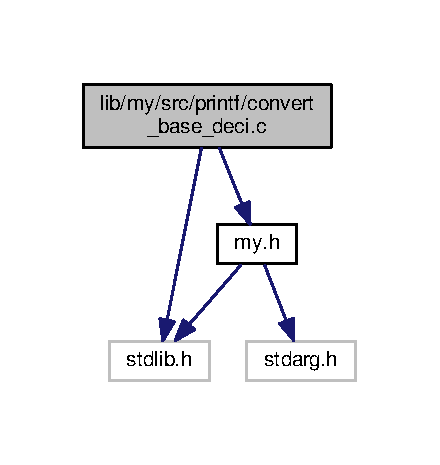
\includegraphics[width=211pt]{convert__base__deci_8c__incl}
\end{center}
\end{figure}
\subsection*{Functions}
\begin{DoxyCompactItemize}
\item 
int \hyperlink{convert__base__deci_8c_adea09e51c1d16f60e2b8b0e82dabc36a}{convert\+\_\+base\+\_\+deci\+\_\+8\+\_\+unint} (unsigned int nb)
\item 
int \hyperlink{convert__base__deci_8c_a8ef7b5028c3c516852da8e8d3bd8f3ab}{convert\+\_\+base\+\_\+deci\+\_\+16\+\_\+un} (unsigned int nb, char $\ast$str)
\item 
int \hyperlink{convert__base__deci_8c_ae76792ea9d72b89dd22b63818937cf6f}{convert\+\_\+base\+\_\+deci\+\_\+16} (long nb, char $\ast$str)
\end{DoxyCompactItemize}


\subsection{Function Documentation}
\hypertarget{convert__base__deci_8c_ae76792ea9d72b89dd22b63818937cf6f}{\index{convert\+\_\+base\+\_\+deci.\+c@{convert\+\_\+base\+\_\+deci.\+c}!convert\+\_\+base\+\_\+deci\+\_\+16@{convert\+\_\+base\+\_\+deci\+\_\+16}}
\index{convert\+\_\+base\+\_\+deci\+\_\+16@{convert\+\_\+base\+\_\+deci\+\_\+16}!convert\+\_\+base\+\_\+deci.\+c@{convert\+\_\+base\+\_\+deci.\+c}}
\subsubsection[{convert\+\_\+base\+\_\+deci\+\_\+16}]{\setlength{\rightskip}{0pt plus 5cm}int convert\+\_\+base\+\_\+deci\+\_\+16 (
\begin{DoxyParamCaption}
\item[{long}]{nb, }
\item[{char $\ast$}]{str}
\end{DoxyParamCaption}
)}}\label{convert__base__deci_8c_ae76792ea9d72b89dd22b63818937cf6f}


Definition at line 67 of file convert\+\_\+base\+\_\+deci.\+c.

\hypertarget{convert__base__deci_8c_a8ef7b5028c3c516852da8e8d3bd8f3ab}{\index{convert\+\_\+base\+\_\+deci.\+c@{convert\+\_\+base\+\_\+deci.\+c}!convert\+\_\+base\+\_\+deci\+\_\+16\+\_\+un@{convert\+\_\+base\+\_\+deci\+\_\+16\+\_\+un}}
\index{convert\+\_\+base\+\_\+deci\+\_\+16\+\_\+un@{convert\+\_\+base\+\_\+deci\+\_\+16\+\_\+un}!convert\+\_\+base\+\_\+deci.\+c@{convert\+\_\+base\+\_\+deci.\+c}}
\subsubsection[{convert\+\_\+base\+\_\+deci\+\_\+16\+\_\+un}]{\setlength{\rightskip}{0pt plus 5cm}int convert\+\_\+base\+\_\+deci\+\_\+16\+\_\+un (
\begin{DoxyParamCaption}
\item[{unsigned int}]{nb, }
\item[{char $\ast$}]{str}
\end{DoxyParamCaption}
)}}\label{convert__base__deci_8c_a8ef7b5028c3c516852da8e8d3bd8f3ab}


Definition at line 40 of file convert\+\_\+base\+\_\+deci.\+c.

\hypertarget{convert__base__deci_8c_adea09e51c1d16f60e2b8b0e82dabc36a}{\index{convert\+\_\+base\+\_\+deci.\+c@{convert\+\_\+base\+\_\+deci.\+c}!convert\+\_\+base\+\_\+deci\+\_\+8\+\_\+unint@{convert\+\_\+base\+\_\+deci\+\_\+8\+\_\+unint}}
\index{convert\+\_\+base\+\_\+deci\+\_\+8\+\_\+unint@{convert\+\_\+base\+\_\+deci\+\_\+8\+\_\+unint}!convert\+\_\+base\+\_\+deci.\+c@{convert\+\_\+base\+\_\+deci.\+c}}
\subsubsection[{convert\+\_\+base\+\_\+deci\+\_\+8\+\_\+unint}]{\setlength{\rightskip}{0pt plus 5cm}int convert\+\_\+base\+\_\+deci\+\_\+8\+\_\+unint (
\begin{DoxyParamCaption}
\item[{unsigned int}]{nb}
\end{DoxyParamCaption}
)}}\label{convert__base__deci_8c_adea09e51c1d16f60e2b8b0e82dabc36a}


Definition at line 14 of file convert\+\_\+base\+\_\+deci.\+c.


\hypertarget{convert__base__unsigned_8c}{\section{lib/my/src/printf/convert\+\_\+base\+\_\+unsigned.c File Reference}
\label{convert__base__unsigned_8c}\index{lib/my/src/printf/convert\+\_\+base\+\_\+unsigned.\+c@{lib/my/src/printf/convert\+\_\+base\+\_\+unsigned.\+c}}
}
{\ttfamily \#include $<$stdlib.\+h$>$}\\*
{\ttfamily \#include \char`\"{}my.\+h\char`\"{}}\\*
Include dependency graph for convert\+\_\+base\+\_\+unsigned.\+c\+:
\nopagebreak
\begin{figure}[H]
\begin{center}
\leavevmode
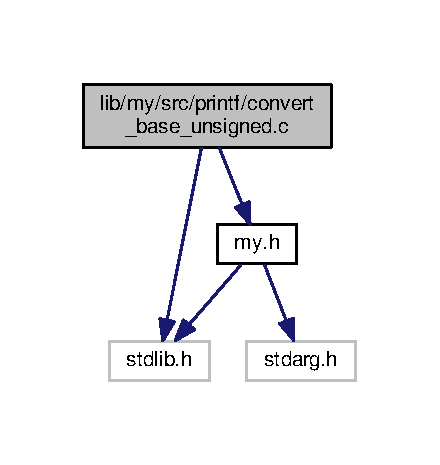
\includegraphics[width=211pt]{convert__base__unsigned_8c__incl}
\end{center}
\end{figure}
\subsection*{Functions}
\begin{DoxyCompactItemize}
\item 
int \hyperlink{convert__base__unsigned_8c_aceed4b7866a7db390bbc5f95524ebbef}{convert\+\_\+base\+\_\+deci\+\_\+16\+\_\+lun} (long unsigned int nb, char $\ast$str)
\item 
void \hyperlink{convert__base__unsigned_8c_aaba0b1edc5014a1d679a115792fc3056}{my\+\_\+rev\+\_\+lunint\+\_\+tab} (long unsigned int $\ast$tab, int i)
\item 
int \hyperlink{convert__base__unsigned_8c_ab1108b223543db15017e7cec0e108b12}{convert\+\_\+base\+\_\+deci\+\_\+8\+\_\+lunint} (long unsigned int nb)
\end{DoxyCompactItemize}


\subsection{Function Documentation}
\hypertarget{convert__base__unsigned_8c_aceed4b7866a7db390bbc5f95524ebbef}{\index{convert\+\_\+base\+\_\+unsigned.\+c@{convert\+\_\+base\+\_\+unsigned.\+c}!convert\+\_\+base\+\_\+deci\+\_\+16\+\_\+lun@{convert\+\_\+base\+\_\+deci\+\_\+16\+\_\+lun}}
\index{convert\+\_\+base\+\_\+deci\+\_\+16\+\_\+lun@{convert\+\_\+base\+\_\+deci\+\_\+16\+\_\+lun}!convert\+\_\+base\+\_\+unsigned.\+c@{convert\+\_\+base\+\_\+unsigned.\+c}}
\subsubsection[{convert\+\_\+base\+\_\+deci\+\_\+16\+\_\+lun}]{\setlength{\rightskip}{0pt plus 5cm}int convert\+\_\+base\+\_\+deci\+\_\+16\+\_\+lun (
\begin{DoxyParamCaption}
\item[{long unsigned int}]{nb, }
\item[{char $\ast$}]{str}
\end{DoxyParamCaption}
)}}\label{convert__base__unsigned_8c_aceed4b7866a7db390bbc5f95524ebbef}


Definition at line 14 of file convert\+\_\+base\+\_\+unsigned.\+c.

\hypertarget{convert__base__unsigned_8c_ab1108b223543db15017e7cec0e108b12}{\index{convert\+\_\+base\+\_\+unsigned.\+c@{convert\+\_\+base\+\_\+unsigned.\+c}!convert\+\_\+base\+\_\+deci\+\_\+8\+\_\+lunint@{convert\+\_\+base\+\_\+deci\+\_\+8\+\_\+lunint}}
\index{convert\+\_\+base\+\_\+deci\+\_\+8\+\_\+lunint@{convert\+\_\+base\+\_\+deci\+\_\+8\+\_\+lunint}!convert\+\_\+base\+\_\+unsigned.\+c@{convert\+\_\+base\+\_\+unsigned.\+c}}
\subsubsection[{convert\+\_\+base\+\_\+deci\+\_\+8\+\_\+lunint}]{\setlength{\rightskip}{0pt plus 5cm}int convert\+\_\+base\+\_\+deci\+\_\+8\+\_\+lunint (
\begin{DoxyParamCaption}
\item[{long unsigned int}]{nb}
\end{DoxyParamCaption}
)}}\label{convert__base__unsigned_8c_ab1108b223543db15017e7cec0e108b12}


Definition at line 51 of file convert\+\_\+base\+\_\+unsigned.\+c.

\hypertarget{convert__base__unsigned_8c_aaba0b1edc5014a1d679a115792fc3056}{\index{convert\+\_\+base\+\_\+unsigned.\+c@{convert\+\_\+base\+\_\+unsigned.\+c}!my\+\_\+rev\+\_\+lunint\+\_\+tab@{my\+\_\+rev\+\_\+lunint\+\_\+tab}}
\index{my\+\_\+rev\+\_\+lunint\+\_\+tab@{my\+\_\+rev\+\_\+lunint\+\_\+tab}!convert\+\_\+base\+\_\+unsigned.\+c@{convert\+\_\+base\+\_\+unsigned.\+c}}
\subsubsection[{my\+\_\+rev\+\_\+lunint\+\_\+tab}]{\setlength{\rightskip}{0pt plus 5cm}void my\+\_\+rev\+\_\+lunint\+\_\+tab (
\begin{DoxyParamCaption}
\item[{long unsigned int $\ast$}]{tab, }
\item[{int}]{i}
\end{DoxyParamCaption}
)}}\label{convert__base__unsigned_8c_aaba0b1edc5014a1d679a115792fc3056}


Definition at line 41 of file convert\+\_\+base\+\_\+unsigned.\+c.


\hypertarget{my__printf_8c}{\section{lib/my/src/printf/my\+\_\+printf.c File Reference}
\label{my__printf_8c}\index{lib/my/src/printf/my\+\_\+printf.\+c@{lib/my/src/printf/my\+\_\+printf.\+c}}
}
{\ttfamily \#include $<$stdarg.\+h$>$}\\*
{\ttfamily \#include \char`\"{}my.\+h\char`\"{}}\\*
Include dependency graph for my\+\_\+printf.\+c\+:
\nopagebreak
\begin{figure}[H]
\begin{center}
\leavevmode
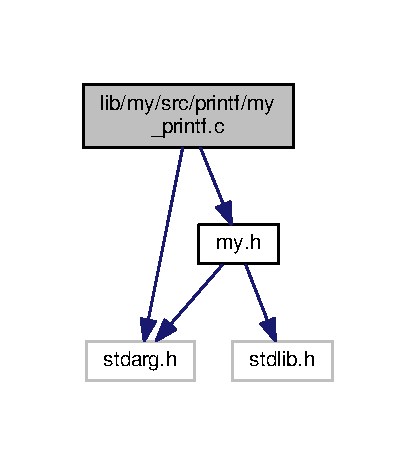
\includegraphics[width=200pt]{my__printf_8c__incl}
\end{center}
\end{figure}
\subsection*{Functions}
\begin{DoxyCompactItemize}
\item 
void \hyperlink{my__printf_8c_a4452e505bf1e5605abf9f93b7659f006}{my\+\_\+printf3} (const char $\ast$format, va\+\_\+list ap, \hyperlink{my_8h_a648ad484eb5d7e8f5d781c45b20f874f}{t\+\_\+index} $\ast$s, const \hyperlink{my_8h_ac25c8b585b5df2bbafd4bdceafa17eb4}{t\+\_\+struc} $\ast$tab)
\item 
void \hyperlink{my__printf_8c_a825e19e51e1de7de0489d41ea79b222f}{my\+\_\+printf2} (const char $\ast$format, va\+\_\+list ap, \hyperlink{my_8h_a648ad484eb5d7e8f5d781c45b20f874f}{t\+\_\+index} $\ast$s, const \hyperlink{my_8h_ac25c8b585b5df2bbafd4bdceafa17eb4}{t\+\_\+struc} $\ast$tab)
\item 
int \hyperlink{my__printf_8c_a8ed3cc79947555e7d13c91bbba84c558}{my\+\_\+printf} (const char $\ast$format,...)
\end{DoxyCompactItemize}


\subsection{Function Documentation}
\hypertarget{my__printf_8c_a8ed3cc79947555e7d13c91bbba84c558}{\index{my\+\_\+printf.\+c@{my\+\_\+printf.\+c}!my\+\_\+printf@{my\+\_\+printf}}
\index{my\+\_\+printf@{my\+\_\+printf}!my\+\_\+printf.\+c@{my\+\_\+printf.\+c}}
\subsubsection[{my\+\_\+printf}]{\setlength{\rightskip}{0pt plus 5cm}int my\+\_\+printf (
\begin{DoxyParamCaption}
\item[{const char $\ast$}]{format, }
\item[{}]{...}
\end{DoxyParamCaption}
)}}\label{my__printf_8c_a8ed3cc79947555e7d13c91bbba84c558}


Definition at line 57 of file my\+\_\+printf.\+c.

\hypertarget{my__printf_8c_a825e19e51e1de7de0489d41ea79b222f}{\index{my\+\_\+printf.\+c@{my\+\_\+printf.\+c}!my\+\_\+printf2@{my\+\_\+printf2}}
\index{my\+\_\+printf2@{my\+\_\+printf2}!my\+\_\+printf.\+c@{my\+\_\+printf.\+c}}
\subsubsection[{my\+\_\+printf2}]{\setlength{\rightskip}{0pt plus 5cm}void my\+\_\+printf2 (
\begin{DoxyParamCaption}
\item[{const char $\ast$}]{format, }
\item[{va\+\_\+list}]{ap, }
\item[{{\bf t\+\_\+index} $\ast$}]{s, }
\item[{const {\bf t\+\_\+struc} $\ast$}]{tab}
\end{DoxyParamCaption}
)}}\label{my__printf_8c_a825e19e51e1de7de0489d41ea79b222f}


Definition at line 34 of file my\+\_\+printf.\+c.

\hypertarget{my__printf_8c_a4452e505bf1e5605abf9f93b7659f006}{\index{my\+\_\+printf.\+c@{my\+\_\+printf.\+c}!my\+\_\+printf3@{my\+\_\+printf3}}
\index{my\+\_\+printf3@{my\+\_\+printf3}!my\+\_\+printf.\+c@{my\+\_\+printf.\+c}}
\subsubsection[{my\+\_\+printf3}]{\setlength{\rightskip}{0pt plus 5cm}void my\+\_\+printf3 (
\begin{DoxyParamCaption}
\item[{const char $\ast$}]{format, }
\item[{va\+\_\+list}]{ap, }
\item[{{\bf t\+\_\+index} $\ast$}]{s, }
\item[{const {\bf t\+\_\+struc} $\ast$}]{tab}
\end{DoxyParamCaption}
)}}\label{my__printf_8c_a4452e505bf1e5605abf9f93b7659f006}


Definition at line 14 of file my\+\_\+printf.\+c.


\hypertarget{my__putchar_8c}{\section{lib/my/src/printf/my\+\_\+putchar.c File Reference}
\label{my__putchar_8c}\index{lib/my/src/printf/my\+\_\+putchar.\+c@{lib/my/src/printf/my\+\_\+putchar.\+c}}
}
{\ttfamily \#include $<$unistd.\+h$>$}\\*
{\ttfamily \#include $<$stdlib.\+h$>$}\\*
{\ttfamily \#include \char`\"{}my.\+h\char`\"{}}\\*
Include dependency graph for my\+\_\+putchar.\+c\+:
\nopagebreak
\begin{figure}[H]
\begin{center}
\leavevmode
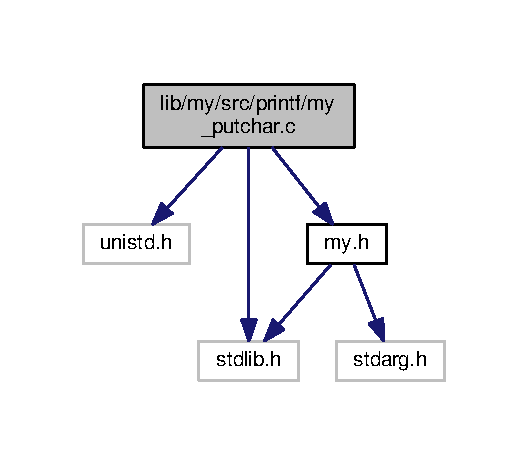
\includegraphics[width=254pt]{my__putchar_8c__incl}
\end{center}
\end{figure}
\subsection*{Functions}
\begin{DoxyCompactItemize}
\item 
void \hyperlink{my__putchar_8c_ac4de74d04dc6e263345755eb62676802}{my\+\_\+putchar} (char c)
\end{DoxyCompactItemize}


\subsection{Function Documentation}
\hypertarget{my__putchar_8c_ac4de74d04dc6e263345755eb62676802}{\index{my\+\_\+putchar.\+c@{my\+\_\+putchar.\+c}!my\+\_\+putchar@{my\+\_\+putchar}}
\index{my\+\_\+putchar@{my\+\_\+putchar}!my\+\_\+putchar.\+c@{my\+\_\+putchar.\+c}}
\subsubsection[{my\+\_\+putchar}]{\setlength{\rightskip}{0pt plus 5cm}void my\+\_\+putchar (
\begin{DoxyParamCaption}
\item[{char}]{c}
\end{DoxyParamCaption}
)}}\label{my__putchar_8c_ac4de74d04dc6e263345755eb62676802}


Definition at line 15 of file my\+\_\+putchar.\+c.


\hypertarget{my__putnbr_8c}{\section{lib/my/src/printf/my\+\_\+putnbr.c File Reference}
\label{my__putnbr_8c}\index{lib/my/src/printf/my\+\_\+putnbr.\+c@{lib/my/src/printf/my\+\_\+putnbr.\+c}}
}
{\ttfamily \#include \char`\"{}my.\+h\char`\"{}}\\*
Include dependency graph for my\+\_\+putnbr.\+c\+:
\nopagebreak
\begin{figure}[H]
\begin{center}
\leavevmode
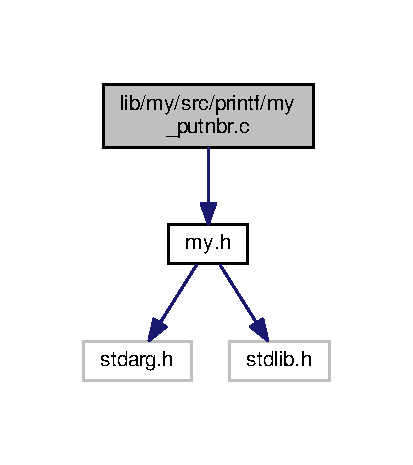
\includegraphics[width=198pt]{my__putnbr_8c__incl}
\end{center}
\end{figure}
\subsection*{Functions}
\begin{DoxyCompactItemize}
\item 
int \hyperlink{my__putnbr_8c_abe11475be3e899d09dd96ff87e27ea33}{my\+\_\+putnbr} (int nb)
\item 
int \hyperlink{my__putnbr_8c_a4a032b76fd1462824c8617c00826036e}{my\+\_\+putnbrnoaffich} (int nb)
\item 
int \hyperlink{my__putnbr_8c_a79d3de06392038b9372c01e0114614a0}{my\+\_\+putnbrs} (int nb, int p, int nbr)
\item 
int \hyperlink{my__putnbr_8c_a536c564648bff72a124a93f152da14c3}{my\+\_\+lunputnbr} (long unsigned int nb)
\end{DoxyCompactItemize}


\subsection{Function Documentation}
\hypertarget{my__putnbr_8c_a536c564648bff72a124a93f152da14c3}{\index{my\+\_\+putnbr.\+c@{my\+\_\+putnbr.\+c}!my\+\_\+lunputnbr@{my\+\_\+lunputnbr}}
\index{my\+\_\+lunputnbr@{my\+\_\+lunputnbr}!my\+\_\+putnbr.\+c@{my\+\_\+putnbr.\+c}}
\subsubsection[{my\+\_\+lunputnbr}]{\setlength{\rightskip}{0pt plus 5cm}int my\+\_\+lunputnbr (
\begin{DoxyParamCaption}
\item[{long unsigned int}]{nb}
\end{DoxyParamCaption}
)}}\label{my__putnbr_8c_a536c564648bff72a124a93f152da14c3}


Definition at line 91 of file my\+\_\+putnbr.\+c.

\hypertarget{my__putnbr_8c_abe11475be3e899d09dd96ff87e27ea33}{\index{my\+\_\+putnbr.\+c@{my\+\_\+putnbr.\+c}!my\+\_\+putnbr@{my\+\_\+putnbr}}
\index{my\+\_\+putnbr@{my\+\_\+putnbr}!my\+\_\+putnbr.\+c@{my\+\_\+putnbr.\+c}}
\subsubsection[{my\+\_\+putnbr}]{\setlength{\rightskip}{0pt plus 5cm}int my\+\_\+putnbr (
\begin{DoxyParamCaption}
\item[{int}]{nb}
\end{DoxyParamCaption}
)}}\label{my__putnbr_8c_abe11475be3e899d09dd96ff87e27ea33}


Definition at line 13 of file my\+\_\+putnbr.\+c.

\hypertarget{my__putnbr_8c_a4a032b76fd1462824c8617c00826036e}{\index{my\+\_\+putnbr.\+c@{my\+\_\+putnbr.\+c}!my\+\_\+putnbrnoaffich@{my\+\_\+putnbrnoaffich}}
\index{my\+\_\+putnbrnoaffich@{my\+\_\+putnbrnoaffich}!my\+\_\+putnbr.\+c@{my\+\_\+putnbr.\+c}}
\subsubsection[{my\+\_\+putnbrnoaffich}]{\setlength{\rightskip}{0pt plus 5cm}int my\+\_\+putnbrnoaffich (
\begin{DoxyParamCaption}
\item[{int}]{nb}
\end{DoxyParamCaption}
)}}\label{my__putnbr_8c_a4a032b76fd1462824c8617c00826036e}


Definition at line 41 of file my\+\_\+putnbr.\+c.

\hypertarget{my__putnbr_8c_a79d3de06392038b9372c01e0114614a0}{\index{my\+\_\+putnbr.\+c@{my\+\_\+putnbr.\+c}!my\+\_\+putnbrs@{my\+\_\+putnbrs}}
\index{my\+\_\+putnbrs@{my\+\_\+putnbrs}!my\+\_\+putnbr.\+c@{my\+\_\+putnbr.\+c}}
\subsubsection[{my\+\_\+putnbrs}]{\setlength{\rightskip}{0pt plus 5cm}int my\+\_\+putnbrs (
\begin{DoxyParamCaption}
\item[{int}]{nb, }
\item[{int}]{p, }
\item[{int}]{nbr}
\end{DoxyParamCaption}
)}}\label{my__putnbr_8c_a79d3de06392038b9372c01e0114614a0}


Definition at line 65 of file my\+\_\+putnbr.\+c.


\hypertarget{my__putstr_8c}{\section{lib/my/src/printf/my\+\_\+putstr.c File Reference}
\label{my__putstr_8c}\index{lib/my/src/printf/my\+\_\+putstr.\+c@{lib/my/src/printf/my\+\_\+putstr.\+c}}
}
{\ttfamily \#include \char`\"{}my.\+h\char`\"{}}\\*
Include dependency graph for my\+\_\+putstr.\+c\+:
\nopagebreak
\begin{figure}[H]
\begin{center}
\leavevmode
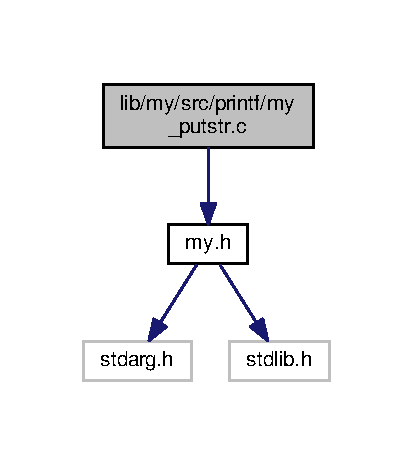
\includegraphics[width=198pt]{my__putstr_8c__incl}
\end{center}
\end{figure}
\subsection*{Functions}
\begin{DoxyCompactItemize}
\item 
int \hyperlink{my__putstr_8c_ac7b78302eb76af4307b2d02f98bd75cb}{my\+\_\+putstr} (char $\ast$str)
\end{DoxyCompactItemize}


\subsection{Function Documentation}
\hypertarget{my__putstr_8c_ac7b78302eb76af4307b2d02f98bd75cb}{\index{my\+\_\+putstr.\+c@{my\+\_\+putstr.\+c}!my\+\_\+putstr@{my\+\_\+putstr}}
\index{my\+\_\+putstr@{my\+\_\+putstr}!my\+\_\+putstr.\+c@{my\+\_\+putstr.\+c}}
\subsubsection[{my\+\_\+putstr}]{\setlength{\rightskip}{0pt plus 5cm}int my\+\_\+putstr (
\begin{DoxyParamCaption}
\item[{char $\ast$}]{str}
\end{DoxyParamCaption}
)}}\label{my__putstr_8c_ac7b78302eb76af4307b2d02f98bd75cb}


Definition at line 13 of file my\+\_\+putstr.\+c.


\hypertarget{my__unputnbr_8c}{\section{lib/my/src/printf/my\+\_\+unputnbr.c File Reference}
\label{my__unputnbr_8c}\index{lib/my/src/printf/my\+\_\+unputnbr.\+c@{lib/my/src/printf/my\+\_\+unputnbr.\+c}}
}
{\ttfamily \#include \char`\"{}my.\+h\char`\"{}}\\*
Include dependency graph for my\+\_\+unputnbr.\+c\+:
\nopagebreak
\begin{figure}[H]
\begin{center}
\leavevmode
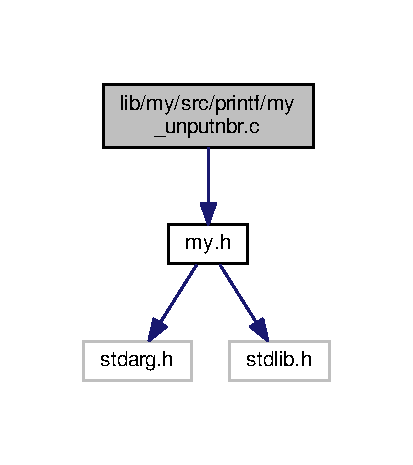
\includegraphics[width=198pt]{my__unputnbr_8c__incl}
\end{center}
\end{figure}
\subsection*{Functions}
\begin{DoxyCompactItemize}
\item 
int \hyperlink{my__unputnbr_8c_a0e2a140625b831447e32a892878b72d7}{my\+\_\+unputnbr} (unsigned int nb)
\item 
int \hyperlink{my__unputnbr_8c_ab0e9c74dd440e1a52cb7f52fdb13c09c}{my\+\_\+unputnbrnoaffich} (unsigned int nb)
\item 
int \hyperlink{my__unputnbr_8c_a9bbf186c3c7f01218fad6ee69cef6b2d}{my\+\_\+unputnbrs} (unsigned int nb, int p, int nbr)
\item 
int \hyperlink{my__unputnbr_8c_a4ea08d997ed58989dca897fefff685dd}{my\+\_\+lputnbr} (long int nb)
\end{DoxyCompactItemize}


\subsection{Function Documentation}
\hypertarget{my__unputnbr_8c_a4ea08d997ed58989dca897fefff685dd}{\index{my\+\_\+unputnbr.\+c@{my\+\_\+unputnbr.\+c}!my\+\_\+lputnbr@{my\+\_\+lputnbr}}
\index{my\+\_\+lputnbr@{my\+\_\+lputnbr}!my\+\_\+unputnbr.\+c@{my\+\_\+unputnbr.\+c}}
\subsubsection[{my\+\_\+lputnbr}]{\setlength{\rightskip}{0pt plus 5cm}int my\+\_\+lputnbr (
\begin{DoxyParamCaption}
\item[{long int}]{nb}
\end{DoxyParamCaption}
)}}\label{my__unputnbr_8c_a4ea08d997ed58989dca897fefff685dd}


Definition at line 77 of file my\+\_\+unputnbr.\+c.

\hypertarget{my__unputnbr_8c_a0e2a140625b831447e32a892878b72d7}{\index{my\+\_\+unputnbr.\+c@{my\+\_\+unputnbr.\+c}!my\+\_\+unputnbr@{my\+\_\+unputnbr}}
\index{my\+\_\+unputnbr@{my\+\_\+unputnbr}!my\+\_\+unputnbr.\+c@{my\+\_\+unputnbr.\+c}}
\subsubsection[{my\+\_\+unputnbr}]{\setlength{\rightskip}{0pt plus 5cm}int my\+\_\+unputnbr (
\begin{DoxyParamCaption}
\item[{unsigned int}]{nb}
\end{DoxyParamCaption}
)}}\label{my__unputnbr_8c_a0e2a140625b831447e32a892878b72d7}


Definition at line 13 of file my\+\_\+unputnbr.\+c.

\hypertarget{my__unputnbr_8c_ab0e9c74dd440e1a52cb7f52fdb13c09c}{\index{my\+\_\+unputnbr.\+c@{my\+\_\+unputnbr.\+c}!my\+\_\+unputnbrnoaffich@{my\+\_\+unputnbrnoaffich}}
\index{my\+\_\+unputnbrnoaffich@{my\+\_\+unputnbrnoaffich}!my\+\_\+unputnbr.\+c@{my\+\_\+unputnbr.\+c}}
\subsubsection[{my\+\_\+unputnbrnoaffich}]{\setlength{\rightskip}{0pt plus 5cm}int my\+\_\+unputnbrnoaffich (
\begin{DoxyParamCaption}
\item[{unsigned int}]{nb}
\end{DoxyParamCaption}
)}}\label{my__unputnbr_8c_ab0e9c74dd440e1a52cb7f52fdb13c09c}


Definition at line 35 of file my\+\_\+unputnbr.\+c.

\hypertarget{my__unputnbr_8c_a9bbf186c3c7f01218fad6ee69cef6b2d}{\index{my\+\_\+unputnbr.\+c@{my\+\_\+unputnbr.\+c}!my\+\_\+unputnbrs@{my\+\_\+unputnbrs}}
\index{my\+\_\+unputnbrs@{my\+\_\+unputnbrs}!my\+\_\+unputnbr.\+c@{my\+\_\+unputnbr.\+c}}
\subsubsection[{my\+\_\+unputnbrs}]{\setlength{\rightskip}{0pt plus 5cm}int my\+\_\+unputnbrs (
\begin{DoxyParamCaption}
\item[{unsigned int}]{nb, }
\item[{int}]{p, }
\item[{int}]{nbr}
\end{DoxyParamCaption}
)}}\label{my__unputnbr_8c_a9bbf186c3c7f01218fad6ee69cef6b2d}


Definition at line 53 of file my\+\_\+unputnbr.\+c.


\hypertarget{get__next__line_8c}{\section{lib/my/src/str/get\+\_\+next\+\_\+line.c File Reference}
\label{get__next__line_8c}\index{lib/my/src/str/get\+\_\+next\+\_\+line.\+c@{lib/my/src/str/get\+\_\+next\+\_\+line.\+c}}
}
{\ttfamily \#include $<$unistd.\+h$>$}\\*
{\ttfamily \#include $<$stdlib.\+h$>$}\\*
{\ttfamily \#include \char`\"{}my.\+h\char`\"{}}\\*
Include dependency graph for get\+\_\+next\+\_\+line.\+c\+:
\nopagebreak
\begin{figure}[H]
\begin{center}
\leavevmode
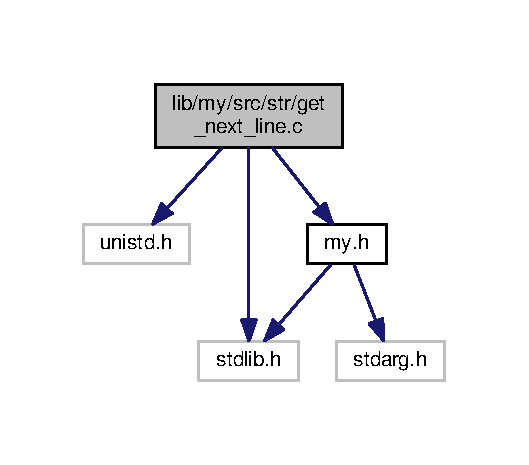
\includegraphics[width=254pt]{get__next__line_8c__incl}
\end{center}
\end{figure}
\subsection*{Functions}
\begin{DoxyCompactItemize}
\item 
void \hyperlink{get__next__line_8c_a9bf3a9107dbcf7a29220551c1fdd07ce}{where\+\_\+my\+\_\+buff\+\_\+end} (char $\ast$statbuffer, char $\ast$stockstat, int j)
\item 
void \hyperlink{get__next__line_8c_a922043af008f3521c98c490bfb92b0b7}{my\+\_\+gstrcpy} (char $\ast$buffer, char $\ast$stockstat, \hyperlink{my_8h_a1670174b47ab43c748df989ae9ef5984}{t\+\_\+getline} $\ast$s, char $\ast$dest)
\item 
char $\ast$ \hyperlink{get__next__line_8c_a7c57c30e5ef063511c69026f042e8c39}{stat\+\_\+in\+\_\+buff} (char $\ast$statbuffer, char $\ast$buffer, \hyperlink{my_8h_a1670174b47ab43c748df989ae9ef5984}{t\+\_\+getline} $\ast$s, char $\ast$dest)
\item 
char $\ast$ \hyperlink{get__next__line_8c_aa36259f17fd04d9decba71955aedeb45}{get\+\_\+next\+\_\+line} (const int fd)
\end{DoxyCompactItemize}


\subsection{Function Documentation}
\hypertarget{get__next__line_8c_aa36259f17fd04d9decba71955aedeb45}{\index{get\+\_\+next\+\_\+line.\+c@{get\+\_\+next\+\_\+line.\+c}!get\+\_\+next\+\_\+line@{get\+\_\+next\+\_\+line}}
\index{get\+\_\+next\+\_\+line@{get\+\_\+next\+\_\+line}!get\+\_\+next\+\_\+line.\+c@{get\+\_\+next\+\_\+line.\+c}}
\subsubsection[{get\+\_\+next\+\_\+line}]{\setlength{\rightskip}{0pt plus 5cm}char$\ast$ get\+\_\+next\+\_\+line (
\begin{DoxyParamCaption}
\item[{const int}]{fd}
\end{DoxyParamCaption}
)}}\label{get__next__line_8c_aa36259f17fd04d9decba71955aedeb45}


Definition at line 81 of file get\+\_\+next\+\_\+line.\+c.

\hypertarget{get__next__line_8c_a922043af008f3521c98c490bfb92b0b7}{\index{get\+\_\+next\+\_\+line.\+c@{get\+\_\+next\+\_\+line.\+c}!my\+\_\+gstrcpy@{my\+\_\+gstrcpy}}
\index{my\+\_\+gstrcpy@{my\+\_\+gstrcpy}!get\+\_\+next\+\_\+line.\+c@{get\+\_\+next\+\_\+line.\+c}}
\subsubsection[{my\+\_\+gstrcpy}]{\setlength{\rightskip}{0pt plus 5cm}void my\+\_\+gstrcpy (
\begin{DoxyParamCaption}
\item[{char $\ast$}]{buffer, }
\item[{char $\ast$}]{stockstat, }
\item[{{\bf t\+\_\+getline} $\ast$}]{s, }
\item[{char $\ast$}]{dest}
\end{DoxyParamCaption}
)}}\label{get__next__line_8c_a922043af008f3521c98c490bfb92b0b7}


Definition at line 29 of file get\+\_\+next\+\_\+line.\+c.

\hypertarget{get__next__line_8c_a7c57c30e5ef063511c69026f042e8c39}{\index{get\+\_\+next\+\_\+line.\+c@{get\+\_\+next\+\_\+line.\+c}!stat\+\_\+in\+\_\+buff@{stat\+\_\+in\+\_\+buff}}
\index{stat\+\_\+in\+\_\+buff@{stat\+\_\+in\+\_\+buff}!get\+\_\+next\+\_\+line.\+c@{get\+\_\+next\+\_\+line.\+c}}
\subsubsection[{stat\+\_\+in\+\_\+buff}]{\setlength{\rightskip}{0pt plus 5cm}char$\ast$ stat\+\_\+in\+\_\+buff (
\begin{DoxyParamCaption}
\item[{char $\ast$}]{statbuffer, }
\item[{char $\ast$}]{buffer, }
\item[{{\bf t\+\_\+getline} $\ast$}]{s, }
\item[{char $\ast$}]{dest}
\end{DoxyParamCaption}
)}}\label{get__next__line_8c_a7c57c30e5ef063511c69026f042e8c39}


Definition at line 55 of file get\+\_\+next\+\_\+line.\+c.

\hypertarget{get__next__line_8c_a9bf3a9107dbcf7a29220551c1fdd07ce}{\index{get\+\_\+next\+\_\+line.\+c@{get\+\_\+next\+\_\+line.\+c}!where\+\_\+my\+\_\+buff\+\_\+end@{where\+\_\+my\+\_\+buff\+\_\+end}}
\index{where\+\_\+my\+\_\+buff\+\_\+end@{where\+\_\+my\+\_\+buff\+\_\+end}!get\+\_\+next\+\_\+line.\+c@{get\+\_\+next\+\_\+line.\+c}}
\subsubsection[{where\+\_\+my\+\_\+buff\+\_\+end}]{\setlength{\rightskip}{0pt plus 5cm}void where\+\_\+my\+\_\+buff\+\_\+end (
\begin{DoxyParamCaption}
\item[{char $\ast$}]{statbuffer, }
\item[{char $\ast$}]{stockstat, }
\item[{int}]{j}
\end{DoxyParamCaption}
)}}\label{get__next__line_8c_a9bf3a9107dbcf7a29220551c1fdd07ce}


Definition at line 15 of file get\+\_\+next\+\_\+line.\+c.


\hypertarget{my__putnstr_8c}{\section{lib/my/src/str/my\+\_\+putnstr.c File Reference}
\label{my__putnstr_8c}\index{lib/my/src/str/my\+\_\+putnstr.\+c@{lib/my/src/str/my\+\_\+putnstr.\+c}}
}
{\ttfamily \#include \char`\"{}my.\+h\char`\"{}}\\*
Include dependency graph for my\+\_\+putnstr.\+c\+:
\nopagebreak
\begin{figure}[H]
\begin{center}
\leavevmode
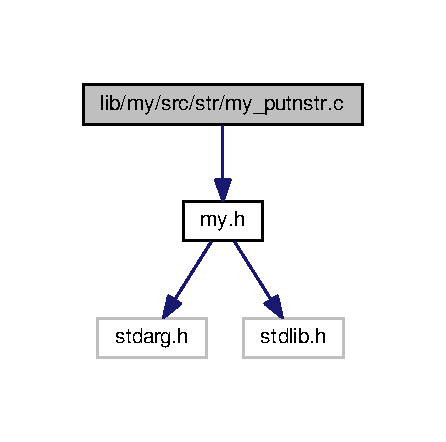
\includegraphics[width=214pt]{my__putnstr_8c__incl}
\end{center}
\end{figure}
\subsection*{Functions}
\begin{DoxyCompactItemize}
\item 
void \hyperlink{my__putnstr_8c_a1290d1e8d903e883482237b8446243dc}{my\+\_\+putnstr} (char $\ast$str, int nb)
\end{DoxyCompactItemize}


\subsection{Function Documentation}
\hypertarget{my__putnstr_8c_a1290d1e8d903e883482237b8446243dc}{\index{my\+\_\+putnstr.\+c@{my\+\_\+putnstr.\+c}!my\+\_\+putnstr@{my\+\_\+putnstr}}
\index{my\+\_\+putnstr@{my\+\_\+putnstr}!my\+\_\+putnstr.\+c@{my\+\_\+putnstr.\+c}}
\subsubsection[{my\+\_\+putnstr}]{\setlength{\rightskip}{0pt plus 5cm}void my\+\_\+putnstr (
\begin{DoxyParamCaption}
\item[{char $\ast$}]{str, }
\item[{int}]{nb}
\end{DoxyParamCaption}
)}}\label{my__putnstr_8c_a1290d1e8d903e883482237b8446243dc}


Definition at line 13 of file my\+\_\+putnstr.\+c.


\hypertarget{my__spe__in__tab_8c}{\section{lib/my/src/str/my\+\_\+spe\+\_\+in\+\_\+tab.c File Reference}
\label{my__spe__in__tab_8c}\index{lib/my/src/str/my\+\_\+spe\+\_\+in\+\_\+tab.\+c@{lib/my/src/str/my\+\_\+spe\+\_\+in\+\_\+tab.\+c}}
}
{\ttfamily \#include $<$stdlib.\+h$>$}\\*
{\ttfamily \#include \char`\"{}my.\+h\char`\"{}}\\*
Include dependency graph for my\+\_\+spe\+\_\+in\+\_\+tab.\+c\+:
\nopagebreak
\begin{figure}[H]
\begin{center}
\leavevmode
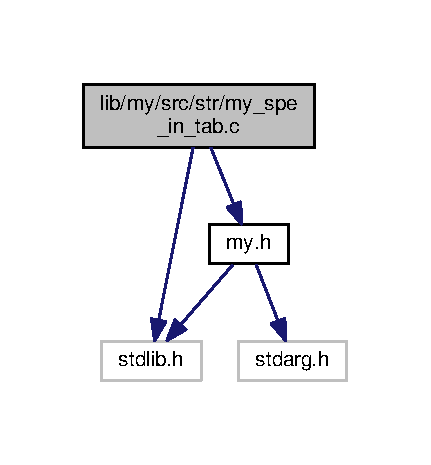
\includegraphics[width=207pt]{my__spe__in__tab_8c__incl}
\end{center}
\end{figure}
\subsection*{Functions}
\begin{DoxyCompactItemize}
\item 
int \hyperlink{my__spe__in__tab_8c_ab4ab3da6597843fbc7ba4938a421797b}{my\+\_\+pstrlen} (char $\ast$str, char sep)
\item 
void \hyperlink{my__spe__in__tab_8c_a9f9f15d9a7706594f0bf134da84f8fcc}{my\+\_\+freetab} (char $\ast$$\ast$tab, int lines)
\item 
char $\ast$$\ast$ \hyperlink{my__spe__in__tab_8c_a95946787f9b07e7299137455e981ea00}{loop\+\_\+condition} (char $\ast$$\ast$tab, \hyperlink{my_8h_a09c3907d6f69f2c69f28b45122bd6a4a}{t\+\_\+win} $\ast$wit, char $\ast$str, char sep)
\item 
char $\ast$$\ast$ \hyperlink{my__spe__in__tab_8c_a8bba86dcfd5fd76f9e59d80bd1354f4e}{my\+\_\+word\+\_\+in\+\_\+tab\+\_\+base} (char $\ast$str, \hyperlink{my_8h_a09c3907d6f69f2c69f28b45122bd6a4a}{t\+\_\+win} $\ast$wit, char sep)
\item 
char $\ast$$\ast$ \hyperlink{my__spe__in__tab_8c_a80c1db0a8b97ae605ef990e4ab025abd}{my\+\_\+spe\+\_\+in\+\_\+tab} (char $\ast$str, char sep)
\end{DoxyCompactItemize}


\subsection{Function Documentation}
\hypertarget{my__spe__in__tab_8c_a95946787f9b07e7299137455e981ea00}{\index{my\+\_\+spe\+\_\+in\+\_\+tab.\+c@{my\+\_\+spe\+\_\+in\+\_\+tab.\+c}!loop\+\_\+condition@{loop\+\_\+condition}}
\index{loop\+\_\+condition@{loop\+\_\+condition}!my\+\_\+spe\+\_\+in\+\_\+tab.\+c@{my\+\_\+spe\+\_\+in\+\_\+tab.\+c}}
\subsubsection[{loop\+\_\+condition}]{\setlength{\rightskip}{0pt plus 5cm}char$\ast$$\ast$ loop\+\_\+condition (
\begin{DoxyParamCaption}
\item[{char $\ast$$\ast$}]{tab, }
\item[{{\bf t\+\_\+win} $\ast$}]{wit, }
\item[{char $\ast$}]{str, }
\item[{char}]{sep}
\end{DoxyParamCaption}
)}}\label{my__spe__in__tab_8c_a95946787f9b07e7299137455e981ea00}


Definition at line 39 of file my\+\_\+spe\+\_\+in\+\_\+tab.\+c.

\hypertarget{my__spe__in__tab_8c_a9f9f15d9a7706594f0bf134da84f8fcc}{\index{my\+\_\+spe\+\_\+in\+\_\+tab.\+c@{my\+\_\+spe\+\_\+in\+\_\+tab.\+c}!my\+\_\+freetab@{my\+\_\+freetab}}
\index{my\+\_\+freetab@{my\+\_\+freetab}!my\+\_\+spe\+\_\+in\+\_\+tab.\+c@{my\+\_\+spe\+\_\+in\+\_\+tab.\+c}}
\subsubsection[{my\+\_\+freetab}]{\setlength{\rightskip}{0pt plus 5cm}void my\+\_\+freetab (
\begin{DoxyParamCaption}
\item[{char $\ast$$\ast$}]{tab, }
\item[{int}]{lines}
\end{DoxyParamCaption}
)}}\label{my__spe__in__tab_8c_a9f9f15d9a7706594f0bf134da84f8fcc}


Definition at line 26 of file my\+\_\+spe\+\_\+in\+\_\+tab.\+c.

\hypertarget{my__spe__in__tab_8c_ab4ab3da6597843fbc7ba4938a421797b}{\index{my\+\_\+spe\+\_\+in\+\_\+tab.\+c@{my\+\_\+spe\+\_\+in\+\_\+tab.\+c}!my\+\_\+pstrlen@{my\+\_\+pstrlen}}
\index{my\+\_\+pstrlen@{my\+\_\+pstrlen}!my\+\_\+spe\+\_\+in\+\_\+tab.\+c@{my\+\_\+spe\+\_\+in\+\_\+tab.\+c}}
\subsubsection[{my\+\_\+pstrlen}]{\setlength{\rightskip}{0pt plus 5cm}int my\+\_\+pstrlen (
\begin{DoxyParamCaption}
\item[{char $\ast$}]{str, }
\item[{char}]{sep}
\end{DoxyParamCaption}
)}}\label{my__spe__in__tab_8c_ab4ab3da6597843fbc7ba4938a421797b}


Definition at line 14 of file my\+\_\+spe\+\_\+in\+\_\+tab.\+c.

\hypertarget{my__spe__in__tab_8c_a80c1db0a8b97ae605ef990e4ab025abd}{\index{my\+\_\+spe\+\_\+in\+\_\+tab.\+c@{my\+\_\+spe\+\_\+in\+\_\+tab.\+c}!my\+\_\+spe\+\_\+in\+\_\+tab@{my\+\_\+spe\+\_\+in\+\_\+tab}}
\index{my\+\_\+spe\+\_\+in\+\_\+tab@{my\+\_\+spe\+\_\+in\+\_\+tab}!my\+\_\+spe\+\_\+in\+\_\+tab.\+c@{my\+\_\+spe\+\_\+in\+\_\+tab.\+c}}
\subsubsection[{my\+\_\+spe\+\_\+in\+\_\+tab}]{\setlength{\rightskip}{0pt plus 5cm}char$\ast$$\ast$ my\+\_\+spe\+\_\+in\+\_\+tab (
\begin{DoxyParamCaption}
\item[{char $\ast$}]{str, }
\item[{char}]{sep}
\end{DoxyParamCaption}
)}}\label{my__spe__in__tab_8c_a80c1db0a8b97ae605ef990e4ab025abd}


Definition at line 83 of file my\+\_\+spe\+\_\+in\+\_\+tab.\+c.

\hypertarget{my__spe__in__tab_8c_a8bba86dcfd5fd76f9e59d80bd1354f4e}{\index{my\+\_\+spe\+\_\+in\+\_\+tab.\+c@{my\+\_\+spe\+\_\+in\+\_\+tab.\+c}!my\+\_\+word\+\_\+in\+\_\+tab\+\_\+base@{my\+\_\+word\+\_\+in\+\_\+tab\+\_\+base}}
\index{my\+\_\+word\+\_\+in\+\_\+tab\+\_\+base@{my\+\_\+word\+\_\+in\+\_\+tab\+\_\+base}!my\+\_\+spe\+\_\+in\+\_\+tab.\+c@{my\+\_\+spe\+\_\+in\+\_\+tab.\+c}}
\subsubsection[{my\+\_\+word\+\_\+in\+\_\+tab\+\_\+base}]{\setlength{\rightskip}{0pt plus 5cm}char$\ast$$\ast$ my\+\_\+word\+\_\+in\+\_\+tab\+\_\+base (
\begin{DoxyParamCaption}
\item[{char $\ast$}]{str, }
\item[{{\bf t\+\_\+win} $\ast$}]{wit, }
\item[{char}]{sep}
\end{DoxyParamCaption}
)}}\label{my__spe__in__tab_8c_a8bba86dcfd5fd76f9e59d80bd1354f4e}


Definition at line 57 of file my\+\_\+spe\+\_\+in\+\_\+tab.\+c.


\hypertarget{my__strcmp_8c}{\section{lib/my/src/str/my\+\_\+strcmp.c File Reference}
\label{my__strcmp_8c}\index{lib/my/src/str/my\+\_\+strcmp.\+c@{lib/my/src/str/my\+\_\+strcmp.\+c}}
}
{\ttfamily \#include \char`\"{}my.\+h\char`\"{}}\\*
Include dependency graph for my\+\_\+strcmp.\+c\+:
\nopagebreak
\begin{figure}[H]
\begin{center}
\leavevmode
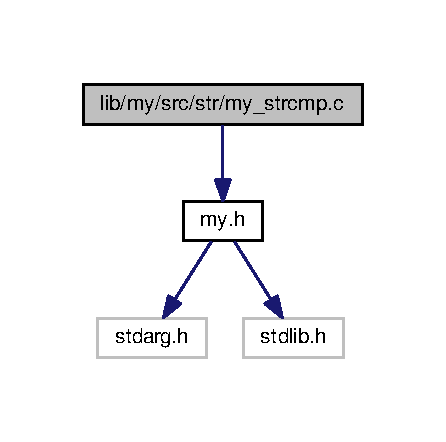
\includegraphics[width=214pt]{my__strcmp_8c__incl}
\end{center}
\end{figure}
\subsection*{Functions}
\begin{DoxyCompactItemize}
\item 
int \hyperlink{my__strcmp_8c_abfc16ef2dad9871456d2f218d60291e5}{my\+\_\+strcmp} (char $\ast$a, char $\ast$b)
\end{DoxyCompactItemize}


\subsection{Function Documentation}
\hypertarget{my__strcmp_8c_abfc16ef2dad9871456d2f218d60291e5}{\index{my\+\_\+strcmp.\+c@{my\+\_\+strcmp.\+c}!my\+\_\+strcmp@{my\+\_\+strcmp}}
\index{my\+\_\+strcmp@{my\+\_\+strcmp}!my\+\_\+strcmp.\+c@{my\+\_\+strcmp.\+c}}
\subsubsection[{my\+\_\+strcmp}]{\setlength{\rightskip}{0pt plus 5cm}int my\+\_\+strcmp (
\begin{DoxyParamCaption}
\item[{char $\ast$}]{a, }
\item[{char $\ast$}]{b}
\end{DoxyParamCaption}
)}}\label{my__strcmp_8c_abfc16ef2dad9871456d2f218d60291e5}


Definition at line 13 of file my\+\_\+strcmp.\+c.


\hypertarget{my__strcpy_8c}{\section{lib/my/src/str/my\+\_\+strcpy.c File Reference}
\label{my__strcpy_8c}\index{lib/my/src/str/my\+\_\+strcpy.\+c@{lib/my/src/str/my\+\_\+strcpy.\+c}}
}
{\ttfamily \#include \char`\"{}my.\+h\char`\"{}}\\*
Include dependency graph for my\+\_\+strcpy.\+c\+:
\nopagebreak
\begin{figure}[H]
\begin{center}
\leavevmode
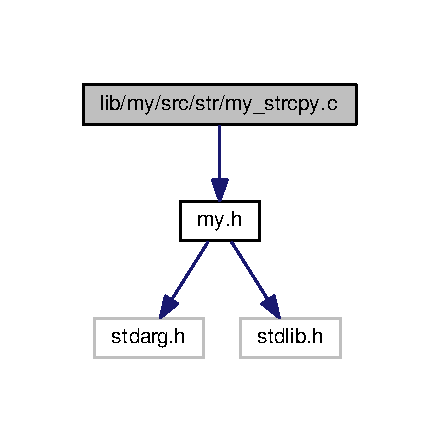
\includegraphics[width=211pt]{my__strcpy_8c__incl}
\end{center}
\end{figure}
\subsection*{Functions}
\begin{DoxyCompactItemize}
\item 
char $\ast$ \hyperlink{my__strcpy_8c_ab9c6a1e01382ed13c4e3a38018322282}{my\+\_\+strcpy} (char $\ast$dest, char $\ast$src)
\end{DoxyCompactItemize}


\subsection{Function Documentation}
\hypertarget{my__strcpy_8c_ab9c6a1e01382ed13c4e3a38018322282}{\index{my\+\_\+strcpy.\+c@{my\+\_\+strcpy.\+c}!my\+\_\+strcpy@{my\+\_\+strcpy}}
\index{my\+\_\+strcpy@{my\+\_\+strcpy}!my\+\_\+strcpy.\+c@{my\+\_\+strcpy.\+c}}
\subsubsection[{my\+\_\+strcpy}]{\setlength{\rightskip}{0pt plus 5cm}char$\ast$ my\+\_\+strcpy (
\begin{DoxyParamCaption}
\item[{char $\ast$}]{dest, }
\item[{char $\ast$}]{src}
\end{DoxyParamCaption}
)}}\label{my__strcpy_8c_ab9c6a1e01382ed13c4e3a38018322282}


Definition at line 13 of file my\+\_\+strcpy.\+c.


\hypertarget{my__strdup_8c}{\section{lib/my/src/str/my\+\_\+strdup.c File Reference}
\label{my__strdup_8c}\index{lib/my/src/str/my\+\_\+strdup.\+c@{lib/my/src/str/my\+\_\+strdup.\+c}}
}
{\ttfamily \#include $<$stdlib.\+h$>$}\\*
{\ttfamily \#include \char`\"{}my.\+h\char`\"{}}\\*
Include dependency graph for my\+\_\+strdup.\+c\+:
\nopagebreak
\begin{figure}[H]
\begin{center}
\leavevmode
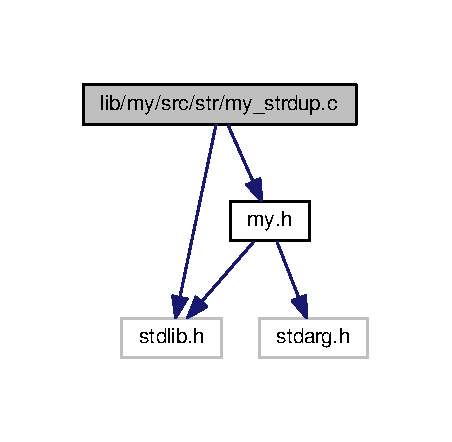
\includegraphics[width=217pt]{my__strdup_8c__incl}
\end{center}
\end{figure}
\subsection*{Functions}
\begin{DoxyCompactItemize}
\item 
char $\ast$ \hyperlink{my__strdup_8c_a4548135c4f1cfcaeff31c8dabb3692d3}{my\+\_\+strdup} (char $\ast$src)
\end{DoxyCompactItemize}


\subsection{Function Documentation}
\hypertarget{my__strdup_8c_a4548135c4f1cfcaeff31c8dabb3692d3}{\index{my\+\_\+strdup.\+c@{my\+\_\+strdup.\+c}!my\+\_\+strdup@{my\+\_\+strdup}}
\index{my\+\_\+strdup@{my\+\_\+strdup}!my\+\_\+strdup.\+c@{my\+\_\+strdup.\+c}}
\subsubsection[{my\+\_\+strdup}]{\setlength{\rightskip}{0pt plus 5cm}char$\ast$ my\+\_\+strdup (
\begin{DoxyParamCaption}
\item[{char $\ast$}]{src}
\end{DoxyParamCaption}
)}}\label{my__strdup_8c_a4548135c4f1cfcaeff31c8dabb3692d3}


Definition at line 14 of file my\+\_\+strdup.\+c.


\hypertarget{my__strglen_8c}{\section{lib/my/src/str/my\+\_\+strglen.c File Reference}
\label{my__strglen_8c}\index{lib/my/src/str/my\+\_\+strglen.\+c@{lib/my/src/str/my\+\_\+strglen.\+c}}
}
{\ttfamily \#include \char`\"{}my.\+h\char`\"{}}\\*
Include dependency graph for my\+\_\+strglen.\+c\+:
\nopagebreak
\begin{figure}[H]
\begin{center}
\leavevmode
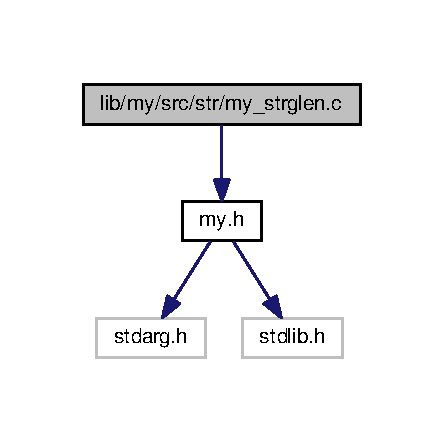
\includegraphics[width=213pt]{my__strglen_8c__incl}
\end{center}
\end{figure}
\subsection*{Functions}
\begin{DoxyCompactItemize}
\item 
int \hyperlink{my__strglen_8c_a0fc216c55eb7277a61f446154aa01017}{my\+\_\+strglen} (long $\ast$a)
\end{DoxyCompactItemize}


\subsection{Function Documentation}
\hypertarget{my__strglen_8c_a0fc216c55eb7277a61f446154aa01017}{\index{my\+\_\+strglen.\+c@{my\+\_\+strglen.\+c}!my\+\_\+strglen@{my\+\_\+strglen}}
\index{my\+\_\+strglen@{my\+\_\+strglen}!my\+\_\+strglen.\+c@{my\+\_\+strglen.\+c}}
\subsubsection[{my\+\_\+strglen}]{\setlength{\rightskip}{0pt plus 5cm}int my\+\_\+strglen (
\begin{DoxyParamCaption}
\item[{long $\ast$}]{a}
\end{DoxyParamCaption}
)}}\label{my__strglen_8c_a0fc216c55eb7277a61f446154aa01017}


Definition at line 13 of file my\+\_\+strglen.\+c.


\hypertarget{my__strlen_8c}{\section{lib/my/src/str/my\+\_\+strlen.c File Reference}
\label{my__strlen_8c}\index{lib/my/src/str/my\+\_\+strlen.\+c@{lib/my/src/str/my\+\_\+strlen.\+c}}
}
\subsection*{Functions}
\begin{DoxyCompactItemize}
\item 
int \hyperlink{my__strlen_8c_ac7e9bd08d068851e31a5b6d408004638}{my\+\_\+strlen} (char $\ast$str)
\end{DoxyCompactItemize}


\subsection{Function Documentation}
\hypertarget{my__strlen_8c_ac7e9bd08d068851e31a5b6d408004638}{\index{my\+\_\+strlen.\+c@{my\+\_\+strlen.\+c}!my\+\_\+strlen@{my\+\_\+strlen}}
\index{my\+\_\+strlen@{my\+\_\+strlen}!my\+\_\+strlen.\+c@{my\+\_\+strlen.\+c}}
\subsubsection[{my\+\_\+strlen}]{\setlength{\rightskip}{0pt plus 5cm}int my\+\_\+strlen (
\begin{DoxyParamCaption}
\item[{char $\ast$}]{str}
\end{DoxyParamCaption}
)}}\label{my__strlen_8c_ac7e9bd08d068851e31a5b6d408004638}


Definition at line 11 of file my\+\_\+strlen.\+c.


\hypertarget{my__strncmp_8c}{\section{lib/my/src/str/my\+\_\+strncmp.c File Reference}
\label{my__strncmp_8c}\index{lib/my/src/str/my\+\_\+strncmp.\+c@{lib/my/src/str/my\+\_\+strncmp.\+c}}
}
\subsection*{Functions}
\begin{DoxyCompactItemize}
\item 
int \hyperlink{my__strncmp_8c_a4f5b9ec850d1c83fd70299ebc2589700}{my\+\_\+strncmp} (char $\ast$a, char $\ast$b, int nb)
\end{DoxyCompactItemize}


\subsection{Function Documentation}
\hypertarget{my__strncmp_8c_a4f5b9ec850d1c83fd70299ebc2589700}{\index{my\+\_\+strncmp.\+c@{my\+\_\+strncmp.\+c}!my\+\_\+strncmp@{my\+\_\+strncmp}}
\index{my\+\_\+strncmp@{my\+\_\+strncmp}!my\+\_\+strncmp.\+c@{my\+\_\+strncmp.\+c}}
\subsubsection[{my\+\_\+strncmp}]{\setlength{\rightskip}{0pt plus 5cm}int my\+\_\+strncmp (
\begin{DoxyParamCaption}
\item[{char $\ast$}]{a, }
\item[{char $\ast$}]{b, }
\item[{int}]{nb}
\end{DoxyParamCaption}
)}}\label{my__strncmp_8c_a4f5b9ec850d1c83fd70299ebc2589700}


Definition at line 11 of file my\+\_\+strncmp.\+c.


\hypertarget{my__strncpy_8c}{\section{lib/my/src/str/my\+\_\+strncpy.c File Reference}
\label{my__strncpy_8c}\index{lib/my/src/str/my\+\_\+strncpy.\+c@{lib/my/src/str/my\+\_\+strncpy.\+c}}
}
{\ttfamily \#include \char`\"{}my.\+h\char`\"{}}\\*
Include dependency graph for my\+\_\+strncpy.\+c\+:
\nopagebreak
\begin{figure}[H]
\begin{center}
\leavevmode
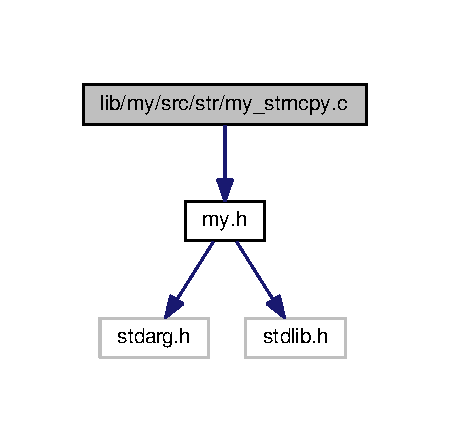
\includegraphics[width=216pt]{my__strncpy_8c__incl}
\end{center}
\end{figure}
\subsection*{Functions}
\begin{DoxyCompactItemize}
\item 
char $\ast$ \hyperlink{my__strncpy_8c_a975053956fdec1e94d9c3764d4e15367}{my\+\_\+strncpy} (char $\ast$dest, char $\ast$src, int nb)
\end{DoxyCompactItemize}


\subsection{Function Documentation}
\hypertarget{my__strncpy_8c_a975053956fdec1e94d9c3764d4e15367}{\index{my\+\_\+strncpy.\+c@{my\+\_\+strncpy.\+c}!my\+\_\+strncpy@{my\+\_\+strncpy}}
\index{my\+\_\+strncpy@{my\+\_\+strncpy}!my\+\_\+strncpy.\+c@{my\+\_\+strncpy.\+c}}
\subsubsection[{my\+\_\+strncpy}]{\setlength{\rightskip}{0pt plus 5cm}char$\ast$ my\+\_\+strncpy (
\begin{DoxyParamCaption}
\item[{char $\ast$}]{dest, }
\item[{char $\ast$}]{src, }
\item[{int}]{nb}
\end{DoxyParamCaption}
)}}\label{my__strncpy_8c_a975053956fdec1e94d9c3764d4e15367}


Definition at line 13 of file my\+\_\+strncpy.\+c.


\hypertarget{my__strndup_8c}{\section{lib/my/src/str/my\+\_\+strndup.c File Reference}
\label{my__strndup_8c}\index{lib/my/src/str/my\+\_\+strndup.\+c@{lib/my/src/str/my\+\_\+strndup.\+c}}
}
{\ttfamily \#include $<$stdlib.\+h$>$}\\*
{\ttfamily \#include \char`\"{}my.\+h\char`\"{}}\\*
Include dependency graph for my\+\_\+strndup.\+c\+:
\nopagebreak
\begin{figure}[H]
\begin{center}
\leavevmode
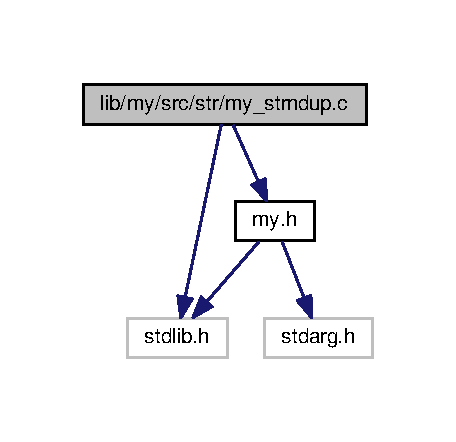
\includegraphics[width=219pt]{my__strndup_8c__incl}
\end{center}
\end{figure}
\subsection*{Functions}
\begin{DoxyCompactItemize}
\item 
char $\ast$ \hyperlink{my__strndup_8c_aa470a7e58967778144f7d737bf64c3e8}{my\+\_\+strndup} (char $\ast$src, int nb)
\end{DoxyCompactItemize}


\subsection{Function Documentation}
\hypertarget{my__strndup_8c_aa470a7e58967778144f7d737bf64c3e8}{\index{my\+\_\+strndup.\+c@{my\+\_\+strndup.\+c}!my\+\_\+strndup@{my\+\_\+strndup}}
\index{my\+\_\+strndup@{my\+\_\+strndup}!my\+\_\+strndup.\+c@{my\+\_\+strndup.\+c}}
\subsubsection[{my\+\_\+strndup}]{\setlength{\rightskip}{0pt plus 5cm}char$\ast$ my\+\_\+strndup (
\begin{DoxyParamCaption}
\item[{char $\ast$}]{src, }
\item[{int}]{nb}
\end{DoxyParamCaption}
)}}\label{my__strndup_8c_aa470a7e58967778144f7d737bf64c3e8}


Definition at line 14 of file my\+\_\+strndup.\+c.


\hypertarget{my__strnscpy_8c}{\section{lib/my/src/str/my\+\_\+strnscpy.c File Reference}
\label{my__strnscpy_8c}\index{lib/my/src/str/my\+\_\+strnscpy.\+c@{lib/my/src/str/my\+\_\+strnscpy.\+c}}
}
{\ttfamily \#include \char`\"{}my.\+h\char`\"{}}\\*
Include dependency graph for my\+\_\+strnscpy.\+c\+:
\nopagebreak
\begin{figure}[H]
\begin{center}
\leavevmode
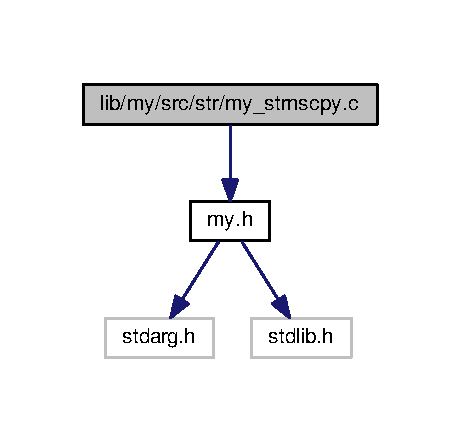
\includegraphics[width=221pt]{my__strnscpy_8c__incl}
\end{center}
\end{figure}
\subsection*{Functions}
\begin{DoxyCompactItemize}
\item 
char $\ast$ \hyperlink{my__strnscpy_8c_a649bba7162650b9189f3051c74545b3a}{my\+\_\+strnscpy} (char $\ast$dest, char $\ast$src, int nb)
\end{DoxyCompactItemize}


\subsection{Function Documentation}
\hypertarget{my__strnscpy_8c_a649bba7162650b9189f3051c74545b3a}{\index{my\+\_\+strnscpy.\+c@{my\+\_\+strnscpy.\+c}!my\+\_\+strnscpy@{my\+\_\+strnscpy}}
\index{my\+\_\+strnscpy@{my\+\_\+strnscpy}!my\+\_\+strnscpy.\+c@{my\+\_\+strnscpy.\+c}}
\subsubsection[{my\+\_\+strnscpy}]{\setlength{\rightskip}{0pt plus 5cm}char$\ast$ my\+\_\+strnscpy (
\begin{DoxyParamCaption}
\item[{char $\ast$}]{dest, }
\item[{char $\ast$}]{src, }
\item[{int}]{nb}
\end{DoxyParamCaption}
)}}\label{my__strnscpy_8c_a649bba7162650b9189f3051c74545b3a}


Definition at line 13 of file my\+\_\+strnscpy.\+c.


\hypertarget{my__strnsdup_8c}{\section{lib/my/src/str/my\+\_\+strnsdup.c File Reference}
\label{my__strnsdup_8c}\index{lib/my/src/str/my\+\_\+strnsdup.\+c@{lib/my/src/str/my\+\_\+strnsdup.\+c}}
}
{\ttfamily \#include $<$stdlib.\+h$>$}\\*
{\ttfamily \#include \char`\"{}my.\+h\char`\"{}}\\*
Include dependency graph for my\+\_\+strnsdup.\+c\+:
\nopagebreak
\begin{figure}[H]
\begin{center}
\leavevmode
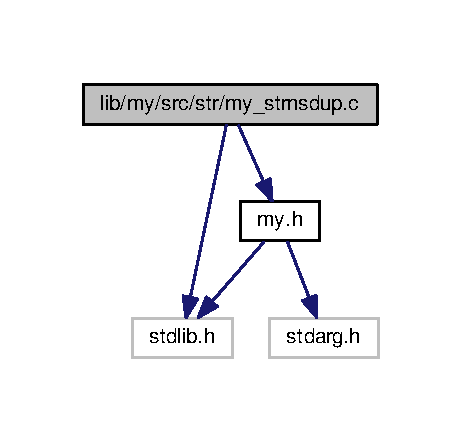
\includegraphics[width=222pt]{my__strnsdup_8c__incl}
\end{center}
\end{figure}
\subsection*{Functions}
\begin{DoxyCompactItemize}
\item 
char $\ast$ \hyperlink{my__strnsdup_8c_a04349ba349d2ec7aece9350d01b1eaf1}{my\+\_\+strnsdup} (char $\ast$src, int nb)
\end{DoxyCompactItemize}


\subsection{Function Documentation}
\hypertarget{my__strnsdup_8c_a04349ba349d2ec7aece9350d01b1eaf1}{\index{my\+\_\+strnsdup.\+c@{my\+\_\+strnsdup.\+c}!my\+\_\+strnsdup@{my\+\_\+strnsdup}}
\index{my\+\_\+strnsdup@{my\+\_\+strnsdup}!my\+\_\+strnsdup.\+c@{my\+\_\+strnsdup.\+c}}
\subsubsection[{my\+\_\+strnsdup}]{\setlength{\rightskip}{0pt plus 5cm}char$\ast$ my\+\_\+strnsdup (
\begin{DoxyParamCaption}
\item[{char $\ast$}]{src, }
\item[{int}]{nb}
\end{DoxyParamCaption}
)}}\label{my__strnsdup_8c_a04349ba349d2ec7aece9350d01b1eaf1}


Definition at line 14 of file my\+\_\+strnsdup.\+c.


\hypertarget{my__tablen_8c}{\section{lib/my/src/str/my\+\_\+tablen.c File Reference}
\label{my__tablen_8c}\index{lib/my/src/str/my\+\_\+tablen.\+c@{lib/my/src/str/my\+\_\+tablen.\+c}}
}
\subsection*{Functions}
\begin{DoxyCompactItemize}
\item 
int \hyperlink{my__tablen_8c_a1d2d0c1f7e29f013e2bfb4ecece00811}{my\+\_\+tablen} (char $\ast$$\ast$tab)
\end{DoxyCompactItemize}


\subsection{Function Documentation}
\hypertarget{my__tablen_8c_a1d2d0c1f7e29f013e2bfb4ecece00811}{\index{my\+\_\+tablen.\+c@{my\+\_\+tablen.\+c}!my\+\_\+tablen@{my\+\_\+tablen}}
\index{my\+\_\+tablen@{my\+\_\+tablen}!my\+\_\+tablen.\+c@{my\+\_\+tablen.\+c}}
\subsubsection[{my\+\_\+tablen}]{\setlength{\rightskip}{0pt plus 5cm}int my\+\_\+tablen (
\begin{DoxyParamCaption}
\item[{char $\ast$$\ast$}]{tab}
\end{DoxyParamCaption}
)}}\label{my__tablen_8c_a1d2d0c1f7e29f013e2bfb4ecece00811}


Definition at line 11 of file my\+\_\+tablen.\+c.


\hypertarget{my__word__in__tab_8c}{\section{lib/my/src/str/my\+\_\+word\+\_\+in\+\_\+tab.c File Reference}
\label{my__word__in__tab_8c}\index{lib/my/src/str/my\+\_\+word\+\_\+in\+\_\+tab.\+c@{lib/my/src/str/my\+\_\+word\+\_\+in\+\_\+tab.\+c}}
}
{\ttfamily \#include $<$stdlib.\+h$>$}\\*
{\ttfamily \#include \char`\"{}my.\+h\char`\"{}}\\*
Include dependency graph for my\+\_\+word\+\_\+in\+\_\+tab.\+c\+:
\nopagebreak
\begin{figure}[H]
\begin{center}
\leavevmode
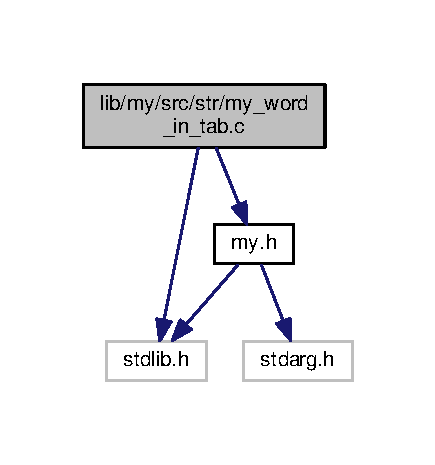
\includegraphics[width=209pt]{my__word__in__tab_8c__incl}
\end{center}
\end{figure}
\subsection*{Functions}
\begin{DoxyCompactItemize}
\item 
int \hyperlink{my__word__in__tab_8c_a5060f96f505bee43cf82cc62caf64c6f}{my\+\_\+pstrlen} (char $\ast$str)
\item 
void \hyperlink{my__word__in__tab_8c_a9f9f15d9a7706594f0bf134da84f8fcc}{my\+\_\+freetab} (char $\ast$$\ast$tab, int lines)
\item 
char $\ast$$\ast$ \hyperlink{my__word__in__tab_8c_a2e8cd60b167a0c0b394a5a97c1cf6433}{loop\+\_\+condition} (char $\ast$$\ast$tab, \hyperlink{my_8h_a09c3907d6f69f2c69f28b45122bd6a4a}{t\+\_\+win} $\ast$wit, char $\ast$str)
\item 
char $\ast$$\ast$ \hyperlink{my__word__in__tab_8c_afc88d903ef92cedd9b8307919007e00b}{my\+\_\+word\+\_\+in\+\_\+tab\+\_\+base} (char $\ast$str, \hyperlink{my_8h_a09c3907d6f69f2c69f28b45122bd6a4a}{t\+\_\+win} $\ast$wit)
\item 
char $\ast$$\ast$ \hyperlink{my__word__in__tab_8c_a7c85d790d5958ef6b7e880acd800fc4f}{my\+\_\+word\+\_\+in\+\_\+tab} (char $\ast$str)
\end{DoxyCompactItemize}


\subsection{Function Documentation}
\hypertarget{my__word__in__tab_8c_a2e8cd60b167a0c0b394a5a97c1cf6433}{\index{my\+\_\+word\+\_\+in\+\_\+tab.\+c@{my\+\_\+word\+\_\+in\+\_\+tab.\+c}!loop\+\_\+condition@{loop\+\_\+condition}}
\index{loop\+\_\+condition@{loop\+\_\+condition}!my\+\_\+word\+\_\+in\+\_\+tab.\+c@{my\+\_\+word\+\_\+in\+\_\+tab.\+c}}
\subsubsection[{loop\+\_\+condition}]{\setlength{\rightskip}{0pt plus 5cm}char$\ast$$\ast$ loop\+\_\+condition (
\begin{DoxyParamCaption}
\item[{char $\ast$$\ast$}]{tab, }
\item[{{\bf t\+\_\+win} $\ast$}]{wit, }
\item[{char $\ast$}]{str}
\end{DoxyParamCaption}
)}}\label{my__word__in__tab_8c_a2e8cd60b167a0c0b394a5a97c1cf6433}


Definition at line 39 of file my\+\_\+word\+\_\+in\+\_\+tab.\+c.

\hypertarget{my__word__in__tab_8c_a9f9f15d9a7706594f0bf134da84f8fcc}{\index{my\+\_\+word\+\_\+in\+\_\+tab.\+c@{my\+\_\+word\+\_\+in\+\_\+tab.\+c}!my\+\_\+freetab@{my\+\_\+freetab}}
\index{my\+\_\+freetab@{my\+\_\+freetab}!my\+\_\+word\+\_\+in\+\_\+tab.\+c@{my\+\_\+word\+\_\+in\+\_\+tab.\+c}}
\subsubsection[{my\+\_\+freetab}]{\setlength{\rightskip}{0pt plus 5cm}void my\+\_\+freetab (
\begin{DoxyParamCaption}
\item[{char $\ast$$\ast$}]{tab, }
\item[{int}]{lines}
\end{DoxyParamCaption}
)}}\label{my__word__in__tab_8c_a9f9f15d9a7706594f0bf134da84f8fcc}


Definition at line 26 of file my\+\_\+word\+\_\+in\+\_\+tab.\+c.

\hypertarget{my__word__in__tab_8c_a5060f96f505bee43cf82cc62caf64c6f}{\index{my\+\_\+word\+\_\+in\+\_\+tab.\+c@{my\+\_\+word\+\_\+in\+\_\+tab.\+c}!my\+\_\+pstrlen@{my\+\_\+pstrlen}}
\index{my\+\_\+pstrlen@{my\+\_\+pstrlen}!my\+\_\+word\+\_\+in\+\_\+tab.\+c@{my\+\_\+word\+\_\+in\+\_\+tab.\+c}}
\subsubsection[{my\+\_\+pstrlen}]{\setlength{\rightskip}{0pt plus 5cm}int my\+\_\+pstrlen (
\begin{DoxyParamCaption}
\item[{char $\ast$}]{str}
\end{DoxyParamCaption}
)}}\label{my__word__in__tab_8c_a5060f96f505bee43cf82cc62caf64c6f}


Definition at line 14 of file my\+\_\+word\+\_\+in\+\_\+tab.\+c.

\hypertarget{my__word__in__tab_8c_a7c85d790d5958ef6b7e880acd800fc4f}{\index{my\+\_\+word\+\_\+in\+\_\+tab.\+c@{my\+\_\+word\+\_\+in\+\_\+tab.\+c}!my\+\_\+word\+\_\+in\+\_\+tab@{my\+\_\+word\+\_\+in\+\_\+tab}}
\index{my\+\_\+word\+\_\+in\+\_\+tab@{my\+\_\+word\+\_\+in\+\_\+tab}!my\+\_\+word\+\_\+in\+\_\+tab.\+c@{my\+\_\+word\+\_\+in\+\_\+tab.\+c}}
\subsubsection[{my\+\_\+word\+\_\+in\+\_\+tab}]{\setlength{\rightskip}{0pt plus 5cm}char$\ast$$\ast$ my\+\_\+word\+\_\+in\+\_\+tab (
\begin{DoxyParamCaption}
\item[{char $\ast$}]{str}
\end{DoxyParamCaption}
)}}\label{my__word__in__tab_8c_a7c85d790d5958ef6b7e880acd800fc4f}


Definition at line 83 of file my\+\_\+word\+\_\+in\+\_\+tab.\+c.

\hypertarget{my__word__in__tab_8c_afc88d903ef92cedd9b8307919007e00b}{\index{my\+\_\+word\+\_\+in\+\_\+tab.\+c@{my\+\_\+word\+\_\+in\+\_\+tab.\+c}!my\+\_\+word\+\_\+in\+\_\+tab\+\_\+base@{my\+\_\+word\+\_\+in\+\_\+tab\+\_\+base}}
\index{my\+\_\+word\+\_\+in\+\_\+tab\+\_\+base@{my\+\_\+word\+\_\+in\+\_\+tab\+\_\+base}!my\+\_\+word\+\_\+in\+\_\+tab.\+c@{my\+\_\+word\+\_\+in\+\_\+tab.\+c}}
\subsubsection[{my\+\_\+word\+\_\+in\+\_\+tab\+\_\+base}]{\setlength{\rightskip}{0pt plus 5cm}char$\ast$$\ast$ my\+\_\+word\+\_\+in\+\_\+tab\+\_\+base (
\begin{DoxyParamCaption}
\item[{char $\ast$}]{str, }
\item[{{\bf t\+\_\+win} $\ast$}]{wit}
\end{DoxyParamCaption}
)}}\label{my__word__in__tab_8c_afc88d903ef92cedd9b8307919007e00b}


Definition at line 57 of file my\+\_\+word\+\_\+in\+\_\+tab.\+c.


\hypertarget{remove__str__in__tab_8c}{\section{lib/my/src/str/remove\+\_\+str\+\_\+in\+\_\+tab.c File Reference}
\label{remove__str__in__tab_8c}\index{lib/my/src/str/remove\+\_\+str\+\_\+in\+\_\+tab.\+c@{lib/my/src/str/remove\+\_\+str\+\_\+in\+\_\+tab.\+c}}
}
{\ttfamily \#include \char`\"{}my.\+h\char`\"{}}\\*
Include dependency graph for remove\+\_\+str\+\_\+in\+\_\+tab.\+c\+:
\nopagebreak
\begin{figure}[H]
\begin{center}
\leavevmode
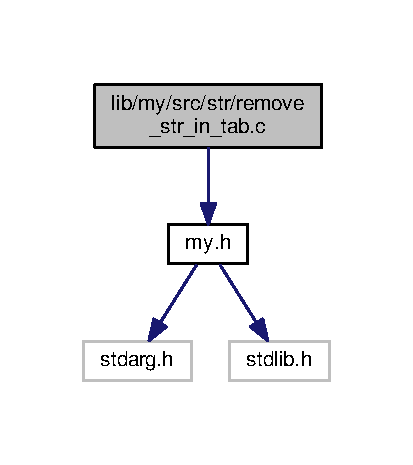
\includegraphics[width=198pt]{remove__str__in__tab_8c__incl}
\end{center}
\end{figure}
\subsection*{Functions}
\begin{DoxyCompactItemize}
\item 
void \hyperlink{remove__str__in__tab_8c_ae07e4d968ee702cb282f6d1235fdecff}{remove\+\_\+str\+\_\+in\+\_\+tab} (char $\ast$$\ast$tab, int x)
\end{DoxyCompactItemize}


\subsection{Function Documentation}
\hypertarget{remove__str__in__tab_8c_ae07e4d968ee702cb282f6d1235fdecff}{\index{remove\+\_\+str\+\_\+in\+\_\+tab.\+c@{remove\+\_\+str\+\_\+in\+\_\+tab.\+c}!remove\+\_\+str\+\_\+in\+\_\+tab@{remove\+\_\+str\+\_\+in\+\_\+tab}}
\index{remove\+\_\+str\+\_\+in\+\_\+tab@{remove\+\_\+str\+\_\+in\+\_\+tab}!remove\+\_\+str\+\_\+in\+\_\+tab.\+c@{remove\+\_\+str\+\_\+in\+\_\+tab.\+c}}
\subsubsection[{remove\+\_\+str\+\_\+in\+\_\+tab}]{\setlength{\rightskip}{0pt plus 5cm}void remove\+\_\+str\+\_\+in\+\_\+tab (
\begin{DoxyParamCaption}
\item[{char $\ast$$\ast$}]{tab, }
\item[{int}]{x}
\end{DoxyParamCaption}
)}}\label{remove__str__in__tab_8c_ae07e4d968ee702cb282f6d1235fdecff}


Definition at line 13 of file remove\+\_\+str\+\_\+in\+\_\+tab.\+c.


\hypertarget{main_8c}{\section{src/main.c File Reference}
\label{main_8c}\index{src/main.\+c@{src/main.\+c}}
}
{\ttfamily \#include \char`\"{}my.\+h\char`\"{}}\\*
{\ttfamily \#include \char`\"{}mysh.\+h\char`\"{}}\\*
Include dependency graph for main.\+c\+:
\nopagebreak
\begin{figure}[H]
\begin{center}
\leavevmode
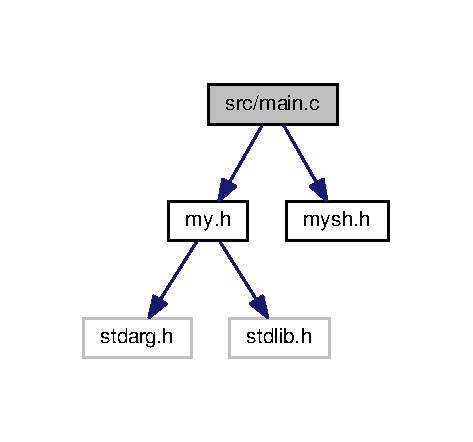
\includegraphics[width=227pt]{main_8c__incl}
\end{center}
\end{figure}
\subsection*{Functions}
\begin{DoxyCompactItemize}
\item 
int \hyperlink{main_8c_a7b26396c9888d66d997b0007e8ff1e60}{main} (int argc, char $\ast$$\ast$argv, char $\ast$$\ast$env)
\end{DoxyCompactItemize}


\subsection{Function Documentation}
\hypertarget{main_8c_a7b26396c9888d66d997b0007e8ff1e60}{\index{main.\+c@{main.\+c}!main@{main}}
\index{main@{main}!main.\+c@{main.\+c}}
\subsubsection[{main}]{\setlength{\rightskip}{0pt plus 5cm}int main (
\begin{DoxyParamCaption}
\item[{int}]{argc, }
\item[{char $\ast$$\ast$}]{argv, }
\item[{char $\ast$$\ast$}]{env}
\end{DoxyParamCaption}
)}}\label{main_8c_a7b26396c9888d66d997b0007e8ff1e60}


Definition at line 14 of file main.\+c.


\hypertarget{my__aff__env_8c}{\section{src/my\+\_\+aff\+\_\+env.c File Reference}
\label{my__aff__env_8c}\index{src/my\+\_\+aff\+\_\+env.\+c@{src/my\+\_\+aff\+\_\+env.\+c}}
}
{\ttfamily \#include \char`\"{}my.\+h\char`\"{}}\\*
{\ttfamily \#include \char`\"{}mysh.\+h\char`\"{}}\\*
{\ttfamily \#include \char`\"{}stdlib.\+h\char`\"{}}\\*
Include dependency graph for my\+\_\+aff\+\_\+env.\+c\+:
\nopagebreak
\begin{figure}[H]
\begin{center}
\leavevmode
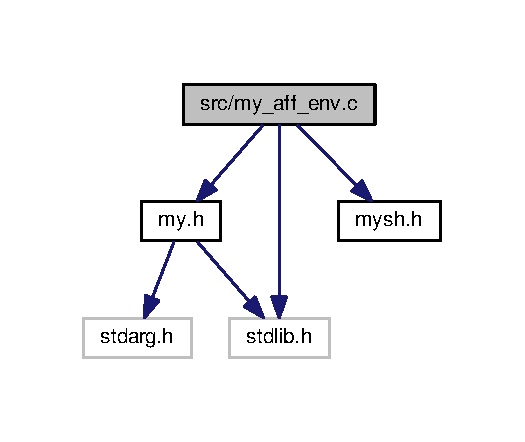
\includegraphics[width=252pt]{my__aff__env_8c__incl}
\end{center}
\end{figure}
\subsection*{Functions}
\begin{DoxyCompactItemize}
\item 
void \hyperlink{my__aff__env_8c_ad8bca16f1928a1facff1dbffe5118774}{my\+\_\+aff\+\_\+env} (char $\ast$$\ast$env)
\end{DoxyCompactItemize}


\subsection{Function Documentation}
\hypertarget{my__aff__env_8c_ad8bca16f1928a1facff1dbffe5118774}{\index{my\+\_\+aff\+\_\+env.\+c@{my\+\_\+aff\+\_\+env.\+c}!my\+\_\+aff\+\_\+env@{my\+\_\+aff\+\_\+env}}
\index{my\+\_\+aff\+\_\+env@{my\+\_\+aff\+\_\+env}!my\+\_\+aff\+\_\+env.\+c@{my\+\_\+aff\+\_\+env.\+c}}
\subsubsection[{my\+\_\+aff\+\_\+env}]{\setlength{\rightskip}{0pt plus 5cm}void my\+\_\+aff\+\_\+env (
\begin{DoxyParamCaption}
\item[{char $\ast$$\ast$}]{env}
\end{DoxyParamCaption}
)}}\label{my__aff__env_8c_ad8bca16f1928a1facff1dbffe5118774}


Definition at line 15 of file my\+\_\+aff\+\_\+env.\+c.


\hypertarget{mysh_8c}{\section{src/mysh.c File Reference}
\label{mysh_8c}\index{src/mysh.\+c@{src/mysh.\+c}}
}
{\ttfamily \#include $<$unistd.\+h$>$}\\*
{\ttfamily \#include $<$stdlib.\+h$>$}\\*
{\ttfamily \#include $<$sys/types.\+h$>$}\\*
{\ttfamily \#include $<$signal.\+h$>$}\\*
{\ttfamily \#include \char`\"{}my.\+h\char`\"{}}\\*
{\ttfamily \#include \char`\"{}mysh.\+h\char`\"{}}\\*
Include dependency graph for mysh.\+c\+:
\nopagebreak
\begin{figure}[H]
\begin{center}
\leavevmode
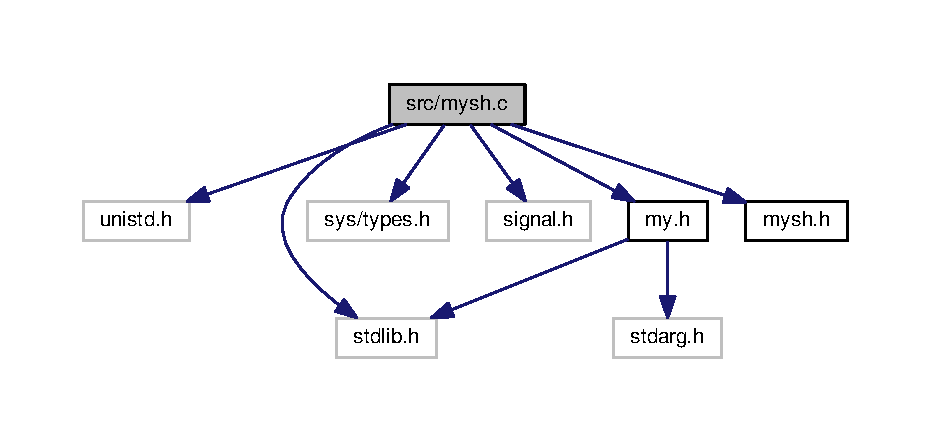
\includegraphics[width=350pt]{mysh_8c__incl}
\end{center}
\end{figure}
\subsection*{Functions}
\begin{DoxyCompactItemize}
\item 
char $\ast$$\ast$ \hyperlink{mysh_8c_a496b9fe4a76f9ff28e287b02b09b6521}{my\+\_\+realloc\+\_\+tab\+\_\+str} (char $\ast$$\ast$tab, int size)
\item 
int \hyperlink{mysh_8c_aba8cbda41e22b44046182ef0f812058a}{my\+\_\+add\+\_\+to\+\_\+tab} (char $\ast$name, char $\ast$$\ast$tab)
\item 
int \hyperlink{mysh_8c_a1420c6c4f6130af4168d5556bb645643}{my\+\_\+unsetenv} (char $\ast$name, char $\ast$$\ast$env)
\item 
void \hyperlink{mysh_8c_a117317c5d13722f8cb100388ce29077b}{my\+\_\+find\+\_\+pwd} (char $\ast$$\ast$env)
\item 
int \hyperlink{mysh_8c_a19cc367c9d4376d9e074531675773419}{case\+\_\+unsetenv} (char $\ast$c, char $\ast$$\ast$env)
\item 
int \hyperlink{mysh_8c_acda6ee77643b3de8db6743e682b7deee}{my\+\_\+setenv} (char $\ast$name, char $\ast$$\ast$env)
\item 
int \hyperlink{mysh_8c_a1ab263b9ed4dab045592ecc7437f0082}{case\+\_\+setenv} (char $\ast$c, char $\ast$$\ast$env)
\item 
int \hyperlink{mysh_8c_a7c1151551f101020fc3999306ba73c69}{case\+\_\+exit} ()
\item 
int \hyperlink{mysh_8c_ab652927dab74a43119141512f578d8d2}{case\+\_\+env} (char $\ast$$\ast$env)
\item 
int \hyperlink{mysh_8c_acb9a87f826c78825c1d808fbce6985a9}{case\+\_\+pwd} (char $\ast$$\ast$env)
\item 
int \hyperlink{mysh_8c_a6d42456eb6a53546a1d5c5850c9cae1d}{my\+\_\+envset\+\_\+fonc} (char $\ast$c, char $\ast$$\ast$env)
\item 
int \hyperlink{mysh_8c_a2fdc7cf8d5b884218e5f3559ce2789d7}{ptr\+\_\+tab\+\_\+fonc} (char $\ast$c, char $\ast$$\ast$env)
\item 
int \hyperlink{mysh_8c_a92bb32d622719b834371dfdacdb56d09}{minishell1} (char $\ast$$\ast$env)
\item 
void \hyperlink{mysh_8c_a12eed0970f97b5ae8dc85cce79a44827}{my\+\_\+prompt} ()
\end{DoxyCompactItemize}


\subsection{Function Documentation}
\hypertarget{mysh_8c_ab652927dab74a43119141512f578d8d2}{\index{mysh.\+c@{mysh.\+c}!case\+\_\+env@{case\+\_\+env}}
\index{case\+\_\+env@{case\+\_\+env}!mysh.\+c@{mysh.\+c}}
\subsubsection[{case\+\_\+env}]{\setlength{\rightskip}{0pt plus 5cm}int case\+\_\+env (
\begin{DoxyParamCaption}
\item[{char $\ast$$\ast$}]{env}
\end{DoxyParamCaption}
)}}\label{mysh_8c_ab652927dab74a43119141512f578d8d2}


Definition at line 166 of file mysh.\+c.

\hypertarget{mysh_8c_a7c1151551f101020fc3999306ba73c69}{\index{mysh.\+c@{mysh.\+c}!case\+\_\+exit@{case\+\_\+exit}}
\index{case\+\_\+exit@{case\+\_\+exit}!mysh.\+c@{mysh.\+c}}
\subsubsection[{case\+\_\+exit}]{\setlength{\rightskip}{0pt plus 5cm}int case\+\_\+exit (
\begin{DoxyParamCaption}
{}
\end{DoxyParamCaption}
)}}\label{mysh_8c_a7c1151551f101020fc3999306ba73c69}


Definition at line 161 of file mysh.\+c.

\hypertarget{mysh_8c_acb9a87f826c78825c1d808fbce6985a9}{\index{mysh.\+c@{mysh.\+c}!case\+\_\+pwd@{case\+\_\+pwd}}
\index{case\+\_\+pwd@{case\+\_\+pwd}!mysh.\+c@{mysh.\+c}}
\subsubsection[{case\+\_\+pwd}]{\setlength{\rightskip}{0pt plus 5cm}int case\+\_\+pwd (
\begin{DoxyParamCaption}
\item[{char $\ast$$\ast$}]{env}
\end{DoxyParamCaption}
)}}\label{mysh_8c_acb9a87f826c78825c1d808fbce6985a9}


Definition at line 172 of file mysh.\+c.

\hypertarget{mysh_8c_a1ab263b9ed4dab045592ecc7437f0082}{\index{mysh.\+c@{mysh.\+c}!case\+\_\+setenv@{case\+\_\+setenv}}
\index{case\+\_\+setenv@{case\+\_\+setenv}!mysh.\+c@{mysh.\+c}}
\subsubsection[{case\+\_\+setenv}]{\setlength{\rightskip}{0pt plus 5cm}int case\+\_\+setenv (
\begin{DoxyParamCaption}
\item[{char $\ast$}]{c, }
\item[{char $\ast$$\ast$}]{env}
\end{DoxyParamCaption}
)}}\label{mysh_8c_a1ab263b9ed4dab045592ecc7437f0082}


Definition at line 139 of file mysh.\+c.

\hypertarget{mysh_8c_a19cc367c9d4376d9e074531675773419}{\index{mysh.\+c@{mysh.\+c}!case\+\_\+unsetenv@{case\+\_\+unsetenv}}
\index{case\+\_\+unsetenv@{case\+\_\+unsetenv}!mysh.\+c@{mysh.\+c}}
\subsubsection[{case\+\_\+unsetenv}]{\setlength{\rightskip}{0pt plus 5cm}int case\+\_\+unsetenv (
\begin{DoxyParamCaption}
\item[{char $\ast$}]{c, }
\item[{char $\ast$$\ast$}]{env}
\end{DoxyParamCaption}
)}}\label{mysh_8c_a19cc367c9d4376d9e074531675773419}


Definition at line 110 of file mysh.\+c.

\hypertarget{mysh_8c_a92bb32d622719b834371dfdacdb56d09}{\index{mysh.\+c@{mysh.\+c}!minishell1@{minishell1}}
\index{minishell1@{minishell1}!mysh.\+c@{mysh.\+c}}
\subsubsection[{minishell1}]{\setlength{\rightskip}{0pt plus 5cm}int minishell1 (
\begin{DoxyParamCaption}
\item[{char $\ast$$\ast$}]{env}
\end{DoxyParamCaption}
)}}\label{mysh_8c_a92bb32d622719b834371dfdacdb56d09}


Definition at line 217 of file mysh.\+c.

\hypertarget{mysh_8c_aba8cbda41e22b44046182ef0f812058a}{\index{mysh.\+c@{mysh.\+c}!my\+\_\+add\+\_\+to\+\_\+tab@{my\+\_\+add\+\_\+to\+\_\+tab}}
\index{my\+\_\+add\+\_\+to\+\_\+tab@{my\+\_\+add\+\_\+to\+\_\+tab}!mysh.\+c@{mysh.\+c}}
\subsubsection[{my\+\_\+add\+\_\+to\+\_\+tab}]{\setlength{\rightskip}{0pt plus 5cm}int my\+\_\+add\+\_\+to\+\_\+tab (
\begin{DoxyParamCaption}
\item[{char $\ast$}]{name, }
\item[{char $\ast$$\ast$}]{tab}
\end{DoxyParamCaption}
)}}\label{mysh_8c_aba8cbda41e22b44046182ef0f812058a}


Definition at line 60 of file mysh.\+c.

\hypertarget{mysh_8c_a6d42456eb6a53546a1d5c5850c9cae1d}{\index{mysh.\+c@{mysh.\+c}!my\+\_\+envset\+\_\+fonc@{my\+\_\+envset\+\_\+fonc}}
\index{my\+\_\+envset\+\_\+fonc@{my\+\_\+envset\+\_\+fonc}!mysh.\+c@{mysh.\+c}}
\subsubsection[{my\+\_\+envset\+\_\+fonc}]{\setlength{\rightskip}{0pt plus 5cm}int my\+\_\+envset\+\_\+fonc (
\begin{DoxyParamCaption}
\item[{char $\ast$}]{c, }
\item[{char $\ast$$\ast$}]{env}
\end{DoxyParamCaption}
)}}\label{mysh_8c_a6d42456eb6a53546a1d5c5850c9cae1d}


Definition at line 178 of file mysh.\+c.

\hypertarget{mysh_8c_a117317c5d13722f8cb100388ce29077b}{\index{mysh.\+c@{mysh.\+c}!my\+\_\+find\+\_\+pwd@{my\+\_\+find\+\_\+pwd}}
\index{my\+\_\+find\+\_\+pwd@{my\+\_\+find\+\_\+pwd}!mysh.\+c@{mysh.\+c}}
\subsubsection[{my\+\_\+find\+\_\+pwd}]{\setlength{\rightskip}{0pt plus 5cm}void my\+\_\+find\+\_\+pwd (
\begin{DoxyParamCaption}
\item[{char $\ast$$\ast$}]{env}
\end{DoxyParamCaption}
)}}\label{mysh_8c_a117317c5d13722f8cb100388ce29077b}


Definition at line 94 of file mysh.\+c.

\hypertarget{mysh_8c_a12eed0970f97b5ae8dc85cce79a44827}{\index{mysh.\+c@{mysh.\+c}!my\+\_\+prompt@{my\+\_\+prompt}}
\index{my\+\_\+prompt@{my\+\_\+prompt}!mysh.\+c@{mysh.\+c}}
\subsubsection[{my\+\_\+prompt}]{\setlength{\rightskip}{0pt plus 5cm}void my\+\_\+prompt (
\begin{DoxyParamCaption}
{}
\end{DoxyParamCaption}
)}}\label{mysh_8c_a12eed0970f97b5ae8dc85cce79a44827}


Definition at line 233 of file mysh.\+c.

\hypertarget{mysh_8c_a496b9fe4a76f9ff28e287b02b09b6521}{\index{mysh.\+c@{mysh.\+c}!my\+\_\+realloc\+\_\+tab\+\_\+str@{my\+\_\+realloc\+\_\+tab\+\_\+str}}
\index{my\+\_\+realloc\+\_\+tab\+\_\+str@{my\+\_\+realloc\+\_\+tab\+\_\+str}!mysh.\+c@{mysh.\+c}}
\subsubsection[{my\+\_\+realloc\+\_\+tab\+\_\+str}]{\setlength{\rightskip}{0pt plus 5cm}char$\ast$$\ast$ my\+\_\+realloc\+\_\+tab\+\_\+str (
\begin{DoxyParamCaption}
\item[{char $\ast$$\ast$}]{tab, }
\item[{int}]{size}
\end{DoxyParamCaption}
)}}\label{mysh_8c_a496b9fe4a76f9ff28e287b02b09b6521}


Definition at line 34 of file mysh.\+c.

\hypertarget{mysh_8c_acda6ee77643b3de8db6743e682b7deee}{\index{mysh.\+c@{mysh.\+c}!my\+\_\+setenv@{my\+\_\+setenv}}
\index{my\+\_\+setenv@{my\+\_\+setenv}!mysh.\+c@{mysh.\+c}}
\subsubsection[{my\+\_\+setenv}]{\setlength{\rightskip}{0pt plus 5cm}int my\+\_\+setenv (
\begin{DoxyParamCaption}
\item[{char $\ast$}]{name, }
\item[{char $\ast$$\ast$}]{env}
\end{DoxyParamCaption}
)}}\label{mysh_8c_acda6ee77643b3de8db6743e682b7deee}


Definition at line 132 of file mysh.\+c.

\hypertarget{mysh_8c_a1420c6c4f6130af4168d5556bb645643}{\index{mysh.\+c@{mysh.\+c}!my\+\_\+unsetenv@{my\+\_\+unsetenv}}
\index{my\+\_\+unsetenv@{my\+\_\+unsetenv}!mysh.\+c@{mysh.\+c}}
\subsubsection[{my\+\_\+unsetenv}]{\setlength{\rightskip}{0pt plus 5cm}int my\+\_\+unsetenv (
\begin{DoxyParamCaption}
\item[{char $\ast$}]{name, }
\item[{char $\ast$$\ast$}]{env}
\end{DoxyParamCaption}
)}}\label{mysh_8c_a1420c6c4f6130af4168d5556bb645643}


Definition at line 74 of file mysh.\+c.

\hypertarget{mysh_8c_a2fdc7cf8d5b884218e5f3559ce2789d7}{\index{mysh.\+c@{mysh.\+c}!ptr\+\_\+tab\+\_\+fonc@{ptr\+\_\+tab\+\_\+fonc}}
\index{ptr\+\_\+tab\+\_\+fonc@{ptr\+\_\+tab\+\_\+fonc}!mysh.\+c@{mysh.\+c}}
\subsubsection[{ptr\+\_\+tab\+\_\+fonc}]{\setlength{\rightskip}{0pt plus 5cm}int ptr\+\_\+tab\+\_\+fonc (
\begin{DoxyParamCaption}
\item[{char $\ast$}]{c, }
\item[{char $\ast$$\ast$}]{env}
\end{DoxyParamCaption}
)}}\label{mysh_8c_a2fdc7cf8d5b884218e5f3559ce2789d7}


Definition at line 193 of file mysh.\+c.


%--- End generated contents ---

% Index
\newpage
\phantomsection
\addcontentsline{toc}{chapter}{Index}
\printindex

\end{document}
